\documentclass{memoir}
\usepackage{import}
\usepackage[utf8]{inputenc}
\usepackage[T1]{fontenc}
\usepackage{lmodern}
\usepackage{tabularx}
\usepackage{booktabs}
\usepackage{longtable}
\usepackage{titling}
\usepackage[svgnames]{xcolor}
\usepackage{enumitem}
\usepackage{tocloft}
\usepackage{subfiles}
\usepackage{graphicx}
\usepackage{float}
\usepackage{svg}
\usepackage{multicol}

\usepackage[centering, margin=1in]{geometry}
\usepackage{afterpage}

\usepackage[sorting=none,backend=biber,style=ieee]{biblatex}
\addbibresource{references.bib}

\usepackage{beuron}
\usepackage{libertine}
\usepackage{libertinust1math}
\usepackage{tcolorbox}

\usepackage{tipa}
\let\altdegree\degree
\let\degree\relax
\usepackage{siunitx}
\DeclareSIUnit\barn{b}

\usepackage[shortcuts]{extdash}

\usepackage{amsmath}
\usepackage{amsfonts}
\usepackage{amssymb}
\usepackage{mathrsfs}
\usepackage{cancel}
\usepackage{slashed}

\allowdisplaybreaks[1]

\usepackage[small, bf, hang]{caption}
\usepackage{subcaption}
\usepackage{url}

\usepackage[arrowdel]{physics}

\usepackage{tensor}
\usepackage[force]{feynmp-auto}
\usepackage{esint}

\usepackage{printlen}

\usepackage{hyperref}
\usepackage{tablefootnote}
\usepackage[noabbrev, nameinlink]{cleveref}
\definecolor{navyblue}{rgb}{0.0, 0.0, 0.5}
% this isn't working???
\hypersetup{
  colorlinks=true,
  linkcolor={red!50!black},
  citecolor={navyblue!50!black},
  urlcolor={navyblue!80!black},
}
\DoubleSpacing

\epigraphfontsize{\small\itshape}
\setlength\epigraphwidth{8cm}
\setlength\epigraphrule{0pt}


\begin{document}
\frontmatter
\thispagestyle{empty}
\pagecolor{navyblue}\afterpage{\nopagecolor}
\color{white}
\vspace*{10pt}
\begin{center}
\Huge\bfseries\scshape
\vspace*{10pt}
\rule{\textwidth}{1pt}
\vspace*{-9pt}
Photoproduction of $K_S$ Pairs at GlueX
\rule{\textwidth}{1pt}
\vfill
\begin{fmffile}{diagram}
\begin{fmfgraph*}(200,200)
    \fmfpen{thick}
    \fmfstraight
    \fmfleftn{i}{2}
    \fmfrightn{o}{3}
    \fmflabel{$p$}{i1}
    \fmflabel{$\gamma$}{i2}
    \fmflabel{$K_S$}{o2}
    \fmflabel{$K_S$}{o3}
    \fmflabel{$p$}{o1}
    \fmf{plain,foreground=white}{i1,t1}
    \fmf{photon,foreground=white}{i2,t2}
    \fmf{plain,foreground=white}{t1,t2}
    \fmf{plain,foreground=white}{t1,v1}
    \fmf{plain,foreground=white}{v1,o1}
    \fmf{phantom}{t2,v2}
    \fmf{phantom}{v2,o3}
    \fmffreeze
    \fmf{plain,label=$X$,foreground=white}{t2,v3}
    \fmf{plain,foreground=white}{v3,o3}
    \fmf{plain,foreground=white}{v3,o2}
    \fmflabel{$p$}{i1}
\end{fmfgraph*}
\end{fmffile}
\vfill
\Huge\bfseries\scshape
Nathaniel Dene Hoffman

Carnegie Mellon University
\end{center}
\color{black}
\clearpage
\begin{KeepFromToc}
    \setcounter{tocdepth}{2}
    \renewcommand{\contentsname}{Table of Contents}
    \tableofcontents
\end{KeepFromToc}
\thispagestyle{empty}
\mainmatter
\chapter{Introduction}
\section{A Brief History of Particle Physics}\label{sec:a_brief_history_of_particle_physics}

Since the days of the ancient Greeks, scientists and philosophers alike have been interested in the fundamental question concerning the composition of the universe. While some Greeks maintained that the world was composed of four indivisible elemental substances (fire, earth, air, and water)~\cite{Ross1925}, this was at best a guess by the early philosophers, who had no systematic mechanism with which to test their theory. Ironically, these philosophers struggled with a question to which modern physicists still have no answer: Are the building blocks of the natural world fundamental (indivisible)~\cite{Hardie1984}?

In 1808, John Dalton published a manuscript which described what is now called the "law of multiple proportions" after compiling several observations on chemical reactions which occur with specific proportions of their reactants. He anglicized the Greek \textit{atomos}, meaning ``not able to be cut'', into the word we are familiar with\textemdash ``atom''~\cite{Dalton1808}. Towards the end of the century, J. J. Thomson demonstrated that cathode rays could be deflected by an electromagnetic field, an observation which could not be explained by an alternative theory that the rays were some form of light~\cite{Thomson1897}. Instead, he proposed that these rays were made up of charged particles he called ``corpuscles'' (later renamed to the familiar ``electrons'')~\cite{Thomson1907}. Around the same time (between 1906 and 1913), Ernest Rutherford, Hans Geiger, and Ernest Marsden conducted experiments in which they scattered alpha particles through a thin metal foil, and, through an analysis of the scattering angles, concluded that a positively charged nucleus must exist at the center of atoms, surrounded by electrons~\cite{Rutherford1911}.

Over the next several decades, the nucleus was further divided into protons and neutrons\footnote{For the discovery of the electron and neutron, Thomson and James Chadwick won Nobel Prizes in Physics in 1906 and 1935, respectively. Rutherford won the 1908 Nobel Prize in Chemistry for his research in radiation. However, I want to emphasize that while I mention the ``big names'' here, there are many who contributed in relative obscurity.}~\cite{Masson1921,Chadwick1932}. In 1964, Murray Gell-Mann and George Zweig proposed a theory that protons and neutrons (and all other baryons and mesons) were in fact composed of smaller particles Gell-Mann called ``quarks''~\cite{Gell-Mann1964}. These particles, along with the electron-like family of leptons (including neutrinos), the gauge bosons, and the Higgs boson, first seen in 2012~\cite{Aad2012}, comprise elements of the Standard Model, a mathematical model which describes all the known forces and matter of the universe, with the notable exceptions (at time of writing) of gravity, dark matter, dark energy, and neutrino masses.

This thesis begins at a time when physicists are working hard to find gaps in this model, mostly by probing higher and higher ranges of energy. The experimental work being done at GlueX, however, resides in a lower energy regime, which we usually describe as ``medium energy physics''. As I will elucidate later in this manuscript, the strong force is non-perturbative in this regime, making direct calculations through the Standard Model all but impossible. However, since the advent of Lattice Quantum Chromodynamics (LQCD) in 1974~\cite{Wilson1974}, physicists have been able to make approximate predictions via computer simulations of the theory.

\section{Thesis Overview}\label{sec:thesis_overview}

Herein, I will focus on a particular portion of the Standard Model that dictates the strong interaction, viz. interactions between quarks and gluons, the mediating gauge boson of the strong force. Beginning with a discussion of the theory and history of $K_S^0$ (K-short) pair production in prior experiments, I will give a brief overview of the GlueX experiment. I will then outline some of the theoretical underpinnings and implications of glueballs to persuade the reader of the importance of this production channel in the larger scheme of GlueX.

Next, I will describe my own analysis, beginning with the layers of data selection which have been carried out to produce a clean sample of events. This will be followed by a discussion of the baryon contributions from excited $\Sigma^+$ hyperons, which were the original focus of my work when this project began. After removing these structures, we will use statistical weighting techniques to remove non-strange backgrounds from the dataset, focusing on the resonances which decay to $K_S^0K_S^0$.

I will then discuss the process of partial-wave analysis (PWA), modeling resonances, and selecting a waveset for my data. I will conclude with the results from fits of these models to the data, the implications of such fits, and the next steps which I or another particle physicist might take in order to illuminate another corner of the light mesonic spectrum.

\section{Motivation}\label{sec:motivation}

While this will be discussed in detail later, I believe it is important to emphasize the motivation for such a study of photoproduction of $K_SK_S$. While the majority of GlueX research concerns the search for hybrid mesons (mesons with valence gluons which contribute to their angular momentum, including ``exotic'' mesons with quantum numbers forbidden by $q\bar{q}$-only states), such mesons cannot be found in this channel, with the possible exception of glueballs, hypothetical bound states made entirely of gluons. Given a bound state of two spin-$\frac{1}{2}$ quarks with relative angular momentum $L$, total spin $S$ and total angular momentum $J$ (the eigenvalue of the operator $\hat{J}^2 = \hat{L}^2 \oplus \hat{S}^2$), we can define the parity operator $\hat{P}$ by its effect on the wave function of the system,
\begin{equation}
  \hat{P}\ket{\vec{r}} = \eta\ket{\vec{r}},
\end{equation}
where $\eta$ can be determined by noting that states of orbital angular momentum are generally proportional to a spherical harmonic in their angular distribution ($\ket{r,\theta,\varphi;LM} \sim Y_L^M(\theta,\varphi)$) and
\begin{equation}
  \hat{P}Y_L^M(\theta,\varphi) = Y_L^M(\pi-\theta,\pi+\varphi) = (-1)^LY_L^M(\theta,\varphi),
\end{equation}
so $\eta = (-1)^L$. The Dirac equation can be used to show that the intrinsic parity of quarks and antiquarks, when multiplied, yields a factor of $-1$, so
\begin{equation}
  \hat{P}\ket{q\bar{q};JLMS} = -(-1)^L.
\end{equation}

Similarly, the charge-conjugation operator $\hat{C}$ (also called C-parity) will introduce a factor of $(-1)^L$ because exchanging charges and other additive quantum numbers of a (neutral\footnote{For $\hat{C}$ to be Hermitian, and thus observable, acting it twice on a state should return the original state, so only eigenvalues of $\pm 1$ are allowed. Therefore, only states which are overall charge neutral are eigenstates of $\hat{C}$.}) quark-antiquark system is akin to reversing their positions under parity. If $\ket{S}$ is antisymmetric under C-parity, we should get an additional factor of $-1$, which is the case for the $S=0$ singlet. With the aformentioned $-1$ due to the intrinsic parity of the quarks and antiquarks, we find
\begin{equation}
  \hat{C}\ket{q\bar{q};JLMS} = (-1)^{L+S}
\end{equation}

Labeling states with the common $J^{PC}$ notation, it can then be shown that states like $0^{--}$, $0^{+-}$, $1^{-+}$, and $2^{+-}$ (among others) are not allowed states for $q\bar{q}$ mesons. As mentioned, the search for such states is a main focus of the GlueX experiment. However, since the particles we are concerned with decays to two identical mesons ($K_S$) which have a symmetric spatial wave function, and because these particles are mesons which follow Bose-Einstein statistics, the angular part of the total wave function must also be symmetric, i.e. $J = \text{even integers}$. Furthermore, because parity is conserved in strong decays, and the state of two identical particles is symmetric under parity, the decaying mesons must also have $P=+$. Finally, the strong interaction also conserves C-parity, and both kaons are neutral, so we can determine the $J^{PC}$ quantum numbers of the resonance to be $\text{even}^{++}$. There should be no overlap here with the aformentioned exotic mesons, but that does not mean the channel is not of interest to GlueX and the larger scientific community. Particularly, the lowest lying glueball states are predicted to not only share these quantum numbers, but exist in the middle of the mass range produced by GlueX energies~\cite{Morningstar1999}. To add to this, the spin-$0$ isospin-$0$ light flavorless mesons, denoted as $f_0$-mesons, may be supernumerary, either due to mixing with a supposed light scalar glueball or by the presence of a light tetraquark or hybrid states (or both)~\cite{Zyla2020}.

However, it would be an understatement to say that the $K_SK_S$ channel at GlueX is not the ideal place to be looking for hybrids, glueballs or tetraquarks. This is because, while we have excellent handles for reconstructing this channel, we have no ability to separate particles of different isospin with these data alone. This means that these $f$ states will be indistinguishable from their isospin-$1$ partners, the $a$-mesons. At first glance, it might seem like a model of the masses of these particles would make it easy to separate them, even if they remained indistinguishable between resonant peaks, but with broad states like the $f_0(1370)$ and states which sit right on top of each other (like the $f_0(980)$ and $a_0(980)$, which interfere with each other), there is likely no unique mass model which can distinguish all of the possible states without relying on data from other channels.

The silver lining is that, due to the GlueX detector's state-of-the-art angular acceptance~\cite{Adhikari2021}, we do stand a chance at separating spin-$0$ states from spin-$2$ states, and GlueX's polarized beam allows us to further understand the mechanisms at play by giving us some indication of the parity of the $t$-channel exchanged particle in the production interaction. We can also use this channel as a proving ground for more complex amplitude analysis involving a mass model, which could be extended to a coupled-channel analysis in the future.


\section{Past Analyses}\label{sec:past-analyses}
The present work is certainly not the first attempt to study $K_S^0$ pair production. The earliest published experiment with a similar final state dates back to 1961, where researchers at CERN measured 54 events which ended in a final state which included two neutral kaons\footnote{Since only $K_S^0$ eigenstates decayed inside the bubble chamber, while the longer lived $K_L^0$ would typically decay somewhere outside the chamber, these experiments infered a final state of $K_S^0K_S^0$. The same can be said for modern experiments, including GlueX.}. For the majority of the 1960s and 1970s, research into this final state was dominated by pion beam production off a proton target, aside from one kaon beam experiment in 1977 (see \Cref{tab:past-analyses}). In the 1980s, several collaborations at DESY began studying electron-positron collisions, which imply an internal virtual photon fusion as the production mechanism. These experiments are an important counterpoint to those involving hadrons, since the glueball does not couple to photons, so any intermediate glueball production in these reactions should be heavily suppressed~\cite{Acciarri2001}, although radial excitations of any glueballs should couple~\cite{Mathieu2009}. While the statistical power of these experiments was very small at first (relative to pion beam experiments), the L3 collaboration at LEP and Belle at KEKB provided larger data samples in the first two decades of the 2000s. Until this study, ITEP and BNL held the statistical lead in non-photon-fusion experiments, and we now present a dataset which is larger than both, even using the most restrictive selections of data.

There has only been one prior experiment, published by the CLAS collaboration in 2018~\cite{Chandavar2018}, which used photoproduction as a means of accessing this channel. While the ``golden channel'' for glueball production remains radiative $J/\psi$ decays to $K_S^0K_S^0\gamma$, since non-glueball intermediate processes converting charm quarks into strange quarks are suppressed, photoproduction could be effective at creating exotic hybrid states as well as glueballs via the photon's hadronic component or Pomeron exchange~\cite{Mathieu2009}. Additionally, the CLAS experiment did not utilize the polarized photon beam capability at JLab, but the current analysis at GlueX does, and this access to linear photon polarization can inform us of the parity exchanged in production of such exotic states. Our dataset is at least $5.7\times$ larger than what was achieved in the CLAS measurement.

\begin{table}
  \begin{center}
    \begin{tabular}{cccc}\toprule
      Channel & Collaboration & \# Events & Year\\\midrule
      $\pi^- p \to K_S^0 K_S^0 n$ & CERN/PS & 54 & 1961~\cite{DiCorato1961}\\
      $\pi^- p \to K_S^0 K_S^0 n$ & BNL & 19 & 1962~\cite{Erwin1962}\\
    $\pi^- p \to K_S^0 K_S^0 n$ & LRL & 66 & 1962~\cite{Alexander1962}\\
    $\pi^- p \to K_S^0 K_S^0 + \text{neutrals}$ & BNL & 374 & 1966~\cite{Crennell1966}\\
  $\pi^- p \to K_S^0 K_S^0 n$ & LRL & 426 & 1966~\cite{Hess1966}\\
  $\pi^- p \to K_S^0 K_S^0 n$ & LRL & 418 & 1967~\cite{Dahl1967}\\
  $\pi^- p \to K_S^0 K_S^0 n$ & CERN/PS & 2559 & 1967~\cite{Beusch1967}\\
  $\pi^- p \to K_S^0 K_S^0 n$ & ANL/ZGS & 1969 & 1968~\cite{Hoang1968} \& 1969~\cite{Hoang1969}\\
$\pi^- p \to K_S^0 K_S^0 n$ & CERN/PS & 4820 & 1975~\cite{Beusch1975}\\
$\pi^- p \to K_S^0 K_S^0 n$ & CERN/PS & 6380 & 1976~\cite{Wetzel1976}\\
$\pi^- p \to K_S^0 K_S^0 n$ & ANL/ZGS & 5096 & 1976~\cite{Cason1976} \& 1979~\cite{Polychronakos1979}\\
$K^- p \to K_S^0 K_S^0 + \text{neutrals}$ & CERN/PS & 410 & 1977~\cite{Barreiro1977}\\
$\pi^- p \to K_S^0 K_S^0 n$ & BNL/MPS & 1278 & 1980~\cite{Gottesman1980}\\
$\pi^- p \to K_S^0 K_S^0 n$ & BNL/MPS & 29381 & 1982~\cite{Etkin1982}\\
$e^+e^- \to e^+e^- K_S^0 K_S^0$ & DESY/TASSO & 100 & 1983~\cite{Althoff1983}\\
$K^-p \to K_S^0K_S^0 Y^*$ & ITEP & 283 & 1986~\cite{Bolonkin1986}\\
$\pi^-p \to K_S^0K_S^0 n$ & ITEP & 7156${}^{\dagger}$ & 1986~\cite{Baloshin1986}\\
    $\pi^- p \to K_S^0 K_S^0 n$ & BNL/MPSII & 40494 & 1986~\cite{Longacre1986}\\
  $e^+e^- \to e^+e^- K_S^0 K_S^0$ & DESY/PLUTO & 21 & 1987~\cite{Berger1988}\\
$K^- p \to K_S^0 K_S^0 \Lambda$ & SLAC/LASS & 441 & 1988~\cite{Aston1988}\\
$e^+e^- \to e^+e^- K_S^0 K_S^0$ & DESY/CELLO & 26 & 1988~\cite{Behrend1989}\\
$e^+e^- \to e^+e^- K_S^0 K_S^0$ & LEP/L3 & 62 & 1995~\cite{Acciarri1995}\\
$pp \to pp K_S^0 K_S^0$ & Fermilab/E690 & 11182 & 1998~\cite{Reyes1998}\\
$\pi^- p \to K_S^0 K_S^0 + \text{neutrals}$ & ITEP & 1000${}^\dagger$ & 1999~\cite{Barkov1999}\\
    $e^+e^- \to e^+e^- K_S^0 K_S^0$ & LEP/L3 & 802 & 2001~\cite{Acciarri2001}\\
  $\pi^- C \to K_S^0 K_S^0 + X$ & ITEP & 553 & 2003~\cite{Tikhomirov2003}\\
      $e^+e^- \to e^+e^- K_S^0 K_S^0$ & LEP/L3 & 870 & 2006~\cite{Schegelsky2006}\\
    $\pi^- p \to K_S^0 K_S^0 n$ & ITEP & 40553 & 2006~\cite{Vladimirsky2006}\\
    $e^+e^- \to e^+e^- K_S^0 K_S^0$ & KEKB/Belle & ???${}^\ddagger$ & 2013~\cite{Uehara2013}\\
    $\gamma p \to K_S^0 K_S^0 p$ & JLAB/CLAS & 13500${}^\dagger$ & 2018~\cite{Chandavar2018}\\
      $\gamma p \to K_S^0 K_S^0 p$ & JLAB/GlueX & 46928${}^\ast$ & 2025 (this analysis)\\\bottomrule
    \end{tabular}
    \caption{Summary of all (known) past analyses involving production of $K_S^0$ pairs. Note that this is possibly not exhaustive and does not include any studies which focus on decays of an intermediate state, i.e. $J/\psi \to \gamma K_S^0K_S^0$.\newline$\dagger$ - Estimated from plots.\newline$\ddagger$ - Reported as three orders of magnitude larger than LEP's result from 2006, but an exact count was difficult to estimate.\newline$\ast$ - Weighted number of events with KinFit $\chi^2_\nu < 3.0$, the standard selection used in this analysis (see \Cref{subsub:kinematic-fit,sec:data-selection}).}\label{tab:past-analyses}
  \end{center}
\end{table}

\chapter{Experimental Design and Data Selection}
\section{The GlueX Experiment}
GlueX, short for the Gluonic Excitation experiment located at the Thomas Jefferson National Accelerator Facility (JLab), first began collecting publication-quality data in 2016 with the goal of establishing the spectrum of light mesonic states including hybrid mesons and glueballs.

\begin{figure}
  \begin{center}
    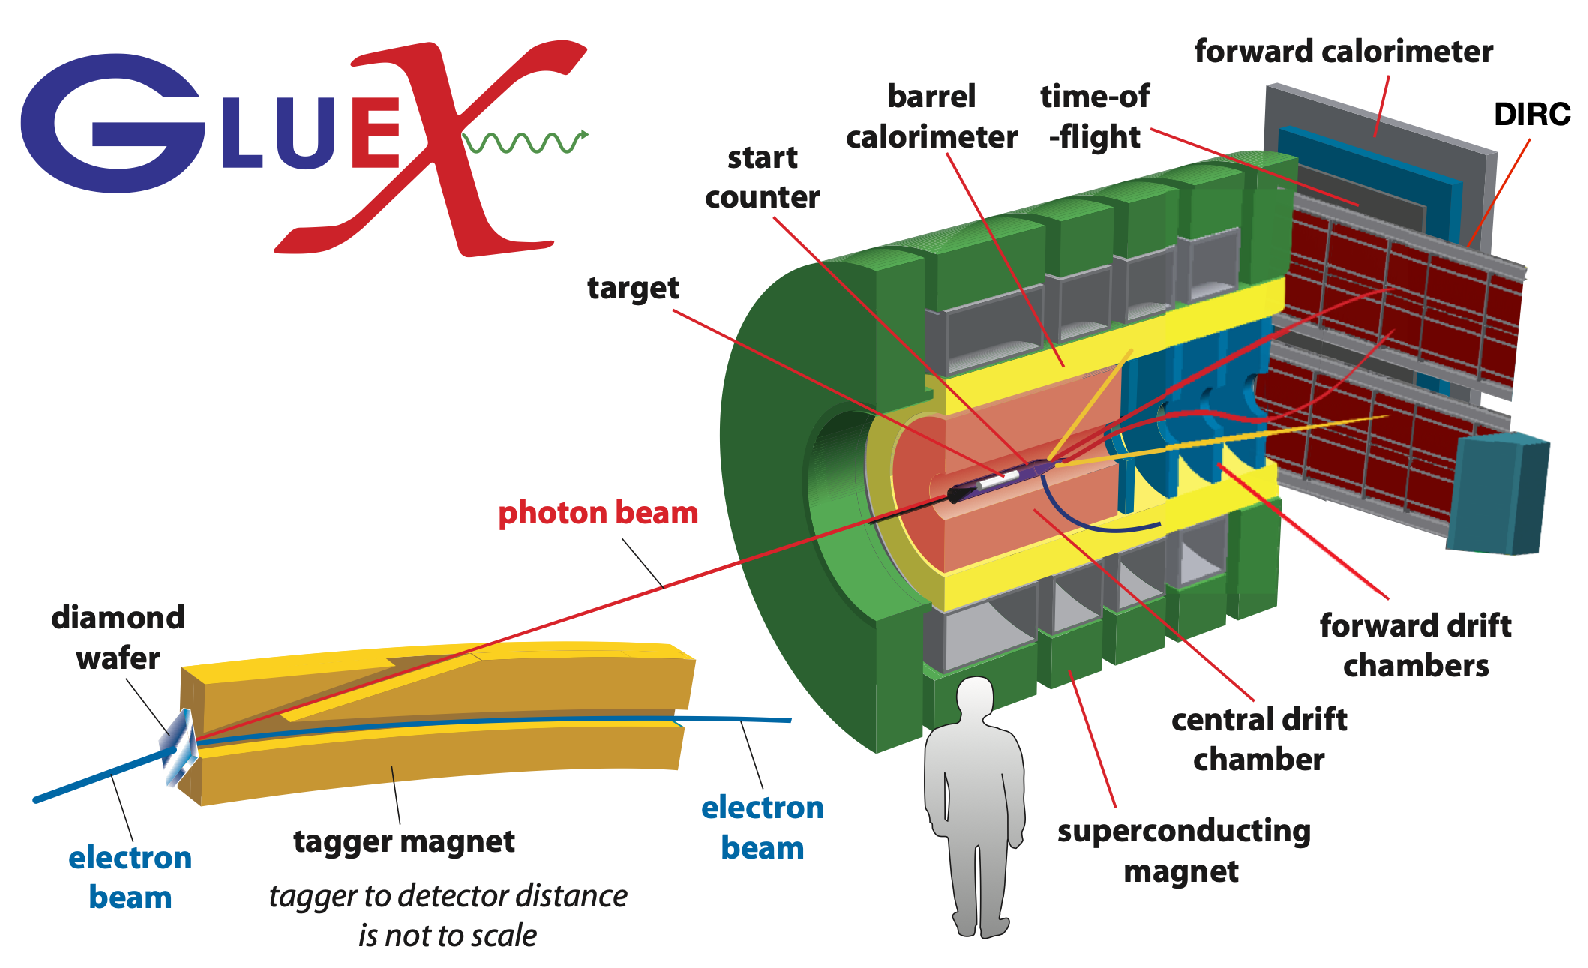
\includegraphics[width=0.8\textwidth]{figures/gluex_detector.png}
  \end{center}
  \caption{A diagram of the GlueX detector at JLab. The DIRC detector was installed in 2019 and was only present for about half of the data analyzed in this study.{\color{red}CITE}}\label{fig:gluex-detector}
\end{figure}

GlueX receives an unpolarized electron beam from the Continuous Electron Beam Accelerator Facility (CEBAF), which is then converted to linearly polarized photons via coherent bremsstrahlung from a diamond radiator (see \Cref{fig:gluex-detector}). The scattering electrons are detected in an array of high-resolution scintillators called the Tagger Microscope (TAGM) which covers beam energies between $8$ and $\SI{9}{\giga\eV}$, a region of energy referred to as the ``coherent peak''. The orientation of the diamond radiator is optimized to produce the highest photon polarization and flux in this region (see \Cref{fig:gluex-polarization}). The rest of the energy range, regions from about $3$--$\SI{8}{\giga\eV}$ and $9$--$\SI{12}{\giga\eV}$, are covered by the lower-resolution Tagger Hodoscope (TAGH). These elements are used to determine only the photon energy, which is equal to the difference between the incident and outgoing electron energies~\cite{adhikari_gluex_2021}.


\begin{figure}
  \begin{center}
    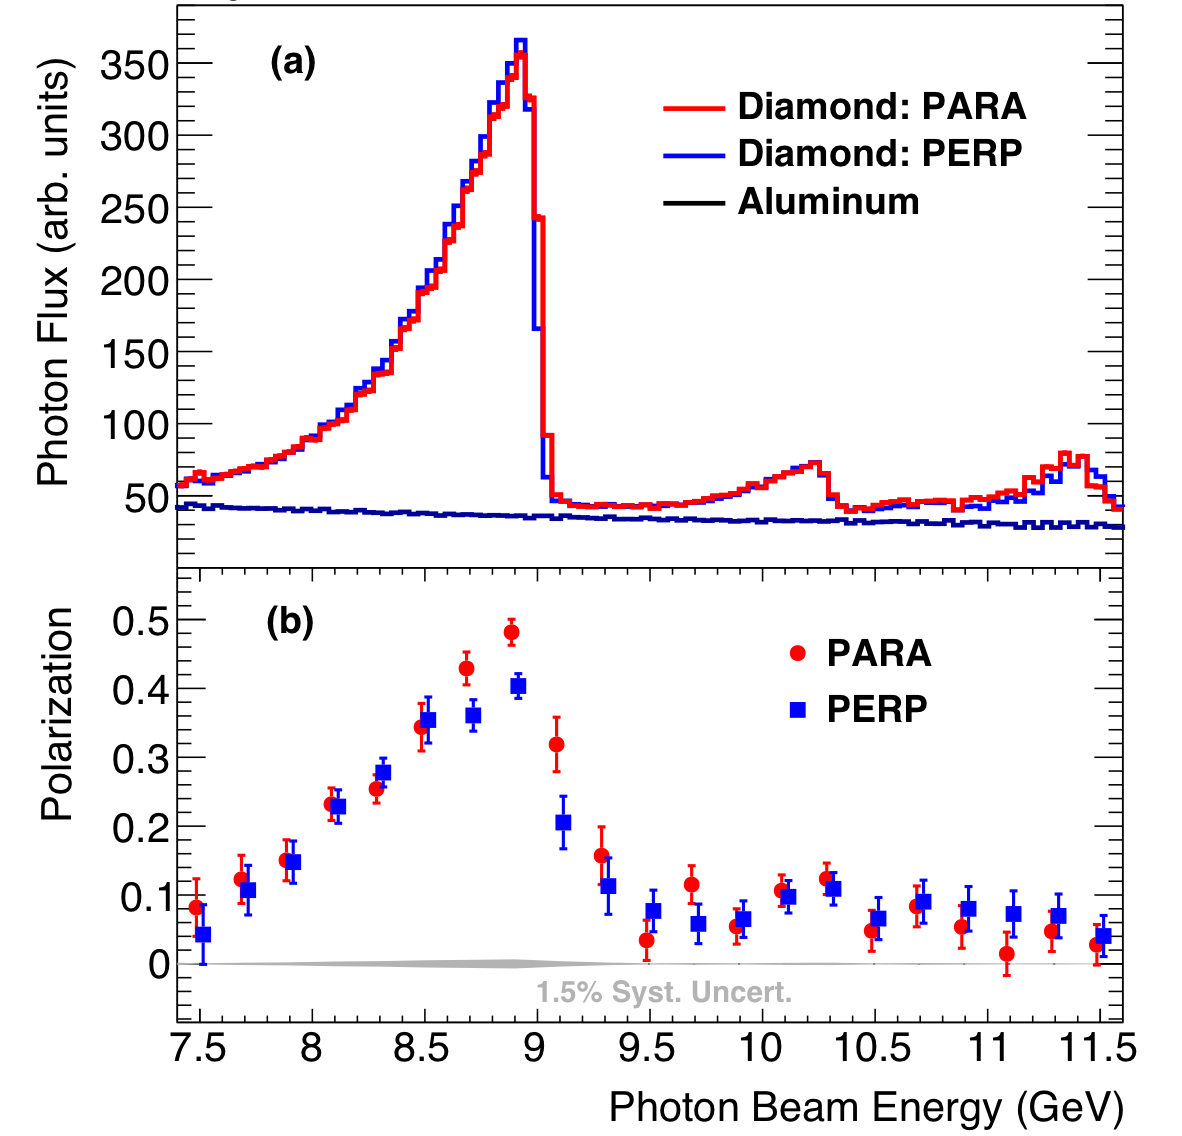
\includegraphics[width=0.95\textwidth]{figures/gluex_polarization.png}
  \end{center}
  \caption{(a) Collimated photon beam intensity versus energy as measured by the Pair Spectrometer. (b) Collimated photon beam polarization as a function of beam energy, as measured by the Triplet Polarimeter, with data points offset horizontally by $\pm\SI{0.015}{\giga\eV}$ for clarity. The labels PARA and PERP refer to orientations of the diamond radiator that result in polarization planes that are parallel and perpendicular to the horizontal, respectively (figure and caption from \cite{adhikari_gluex_2021}).}\label{fig:gluex-polarization}
\end{figure}


\begin{figure}
  \begin{center}
    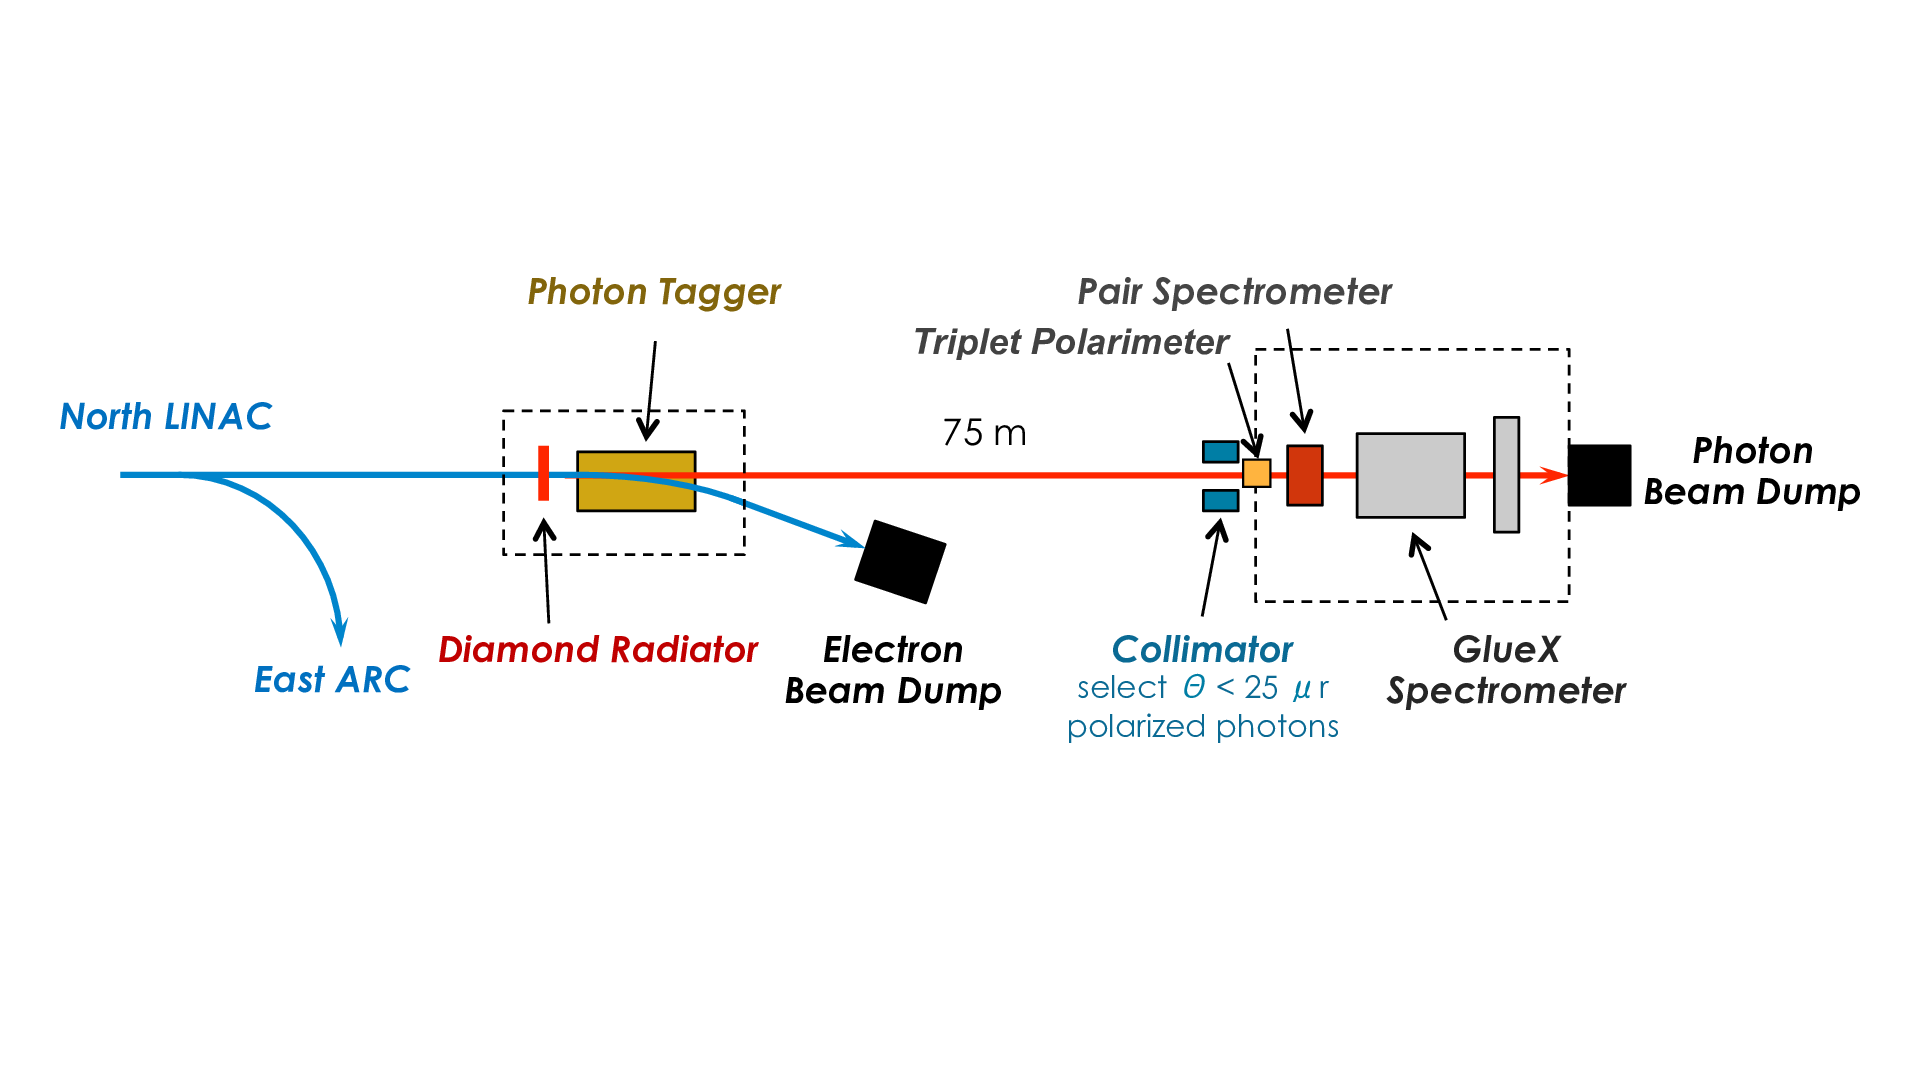
\includegraphics[width=0.95\textwidth]{figures/gluex_beamline.png}
  \end{center}
  \caption{A diagram of the beamline layout of the Triplet Polarimeter (TPOL) and Pair Spectrometer (PS) used to measure the polarization and beam flux.}\label{fig:gluex-beamline}
\end{figure}


To measure the polarization properties of the photon beam as well as the photon flux, the photon beam passes through a thin beryllium foil which induces $e^+e^-$ pair production on some known fraction of the photons (see \Cref{fig:gluex-beamline}). The angular distribution of the produced electrons along with an electron knocked out of the foil medium as part of the pair production process is measured by the Triplet Polarimeter (TPOL) to determine the photon polarization fraction. The Pair Spectrometer (PS) then counts the pair-produced electrons in coincidence with the TAGM and TAGH detectors. A known fraction\footnote{We know the radiation length of the beryllium foil, and this along with the radiator thickness determines the fraction of photons which will pass through without interacting.} of the beam is converted to $e^+e^-$ pairs in this way, allowing for an accurate measurement of the photon flux and the energy dependence of the polarization fraction.

Photons which do not pair-produce in the beryllium radiator interact with a liquid hydrogen cryotarget, which maintains a temperature of $\SI{20.1}{\K}$, allowing the contents to act as a stationary proton target. A set of thin scintillators called the Start Counter (ST) surrounds the target, which captures the initial signals (and azimuthal angles) from reaction products and associates them with the electron radio frequency (RF) beam bunch from which the reaction originated\footnote{The electron beam bunches from the CEBAF arrive every $\SI{4}{\nano\s}$, a rate of $\SI{250}{\mega\hertz}$.}. Any products of the reaction next pass through either the Central Drift Chamber (CDC) or Forward Drift Chamber (FDC) depending on their trajectory (particles within $1^{\circ}$\textendash$10^{\circ}$ of the beamline pass through the FDC, and the detector has partial coverage up to $20^{\circ}$). The CDC is filled with long metal tubes at various orientations, while the FDC chambers are flat disks. Each tube/disk is filled with a gaseous mixture of argon and carbon dioxide\footnote{These particular gases and the mixture ratio are chosen to reduce interfering effects from the magnetic field of the main solenoid.} with a thin wire running through their center of each tube and an array of wires crossing the plane of each disk. The wire and tube/disk faces are held at a voltage differential, and charged particles passing through the chambers ionize the gases inside. The faster-moving electrons move towards the positively charged wires, while the slower-moving ions move towards the tubes/disks. The combination of these signals allows for the reconstruction of the trajectories of each charged particle which passes through each chamber. Both detectors are situated inside a solenoid with a magnetic field around $\SI{2}{\tesla}$, and this field bends the trajectories of charged particles, allowing for proper identification of the sign of the charge as well as the particle's momentum.

The Barrel Calorimeter (BCAL) surrounding the CDC and the Forward Calorimeter (FCAL) in front of the FDC measure the energy of electromagnetic deposits from interactions with charged and neutral particles. This includes photons originating from the decays of light neutral mesons like the $\pi^0$ and $\eta$. Because such neutral particles pass through the CDC and FDC without detection, these calorimeters are necessary for their reconstruction. However, since there are no intermediate trajectories, GlueX is unable to reconstruct the decay vertices of these neutral particles. Since we are studying a reaction with a fully charged final state, this might not seem important. However, in \Cref{sub:neutral-kaon-decay-channels}, we will discuss the study of neutral decays of $K_S^0\to 2\pi^0 \to 4\gamma$, where the reconstruction will be severely limited due to the inability to reconstruct the decay vertex of the $K_S^0$.

There is a final scintillator array called the Time-of-Flight (TOF) detector situated immediately between the FDC and the FCAL. In combination with the ST and the RF timing information from the accelerator, this aids in charged-particle identification via a measurement of the flight time between the two detectors. Additionally, in 2019, an additional detector, the DIRC\footnote{An acronym for Detection of Internally Reflected Cherenkov light} detector was installed between the TOF and FDC to further aid in identification of charged pions and kaons. This detector measures the angle of the cone of Cherenkov radiation emitted by relativistic charged particles, which can be used to ascertain their velocity via the relation $\cos\theta_c \sim 1/v$. When compared to measurements of the particle's momentum, this detector can be used to distinguish pions, kaons, and protons. Further information about the GlueX detector and the DIRC can be found in references \cite{adhikari_gluex_2021} and \cite{ali_installation_2020} respectively.

The data analyzed in this thesis were collected in four separate ``run periods'' across two experiment ``phases'', denoted Phase-I and Phase-II. Phase-I consists of three run periods, notated Spring 2017, Spring 2018, and Fall 2018 by the season and year when data collection began, and Phase-II contains one run period, Spring 2020\footnote{This run technically began at the end of 2019} and is the only dataset which was collected after the DIRC installation. The total luminosity, coherent peak range, and luminosity in the coherent peak for each run period is listed in \Cref{tab:run-info}.


\begin{table}
  \begin{center}
    \begin{tabular}{ccccc}\toprule
      Experiment & Run Period & Luminosity ($E_\gamma > \SI{6.0}{\giga\eV}$) & Coherent Peak Range & Luminosity in Coherent Peak \\\midrule
      Phase-I & Spring 2017 & $\SI{74.7}{\pico\barn^{-1}}$ & $8.2$--$\SI{8.8}{\giga\eV}$ & $\SI{21.8}{\pico\barn^{-1}}$ \\
              & Spring 2018 & $\SI{223.8}{\pico\barn^{-1}}$ & $8.2$--$\SI{8.8}{\giga\eV}$ & $\SI{63.0}{\pico\barn^{-1}}$ \\
              & Fall 2018 & $\SI{141.1}{\pico\barn^{-1}}$ & $8.2$--$\SI{8.8}{\giga\eV}$ & $\SI{40.1}{\pico\barn^{-1}}$ \\\midrule
      Phase-II & Spring 2020 & $\SI{386.2}{\pico\barn^{-1}}$ & $8.0$--$\SI{8.6}{\giga\eV}$ & $\SI{132.4}{\pico\barn^{-1}}$ \\\midrule
      Total & & $\SI{825.8}{\pico\barn^{-1}}$ & & $\SI{257.3}{\pico\barn^{-1}}$ \\\bottomrule
    \end{tabular}
    \caption{Summary of total luminosity and total luminosity in the coherent peak for each run period.}\label{tab:run-info}
  \end{center}
\end{table}

The entire GlueX detector has been simulated with Geant4. Due to small changes and updates to the detector and its simulation between run periods, we will treat these datasets separately during the analysis, only presenting combined results in summary. Therefore, when generating Monte Carlo simulated data to model detector acceptance, each run period must be simulated separately.

\subsection{Particle Identification and the GlueX Kinematic Fit}\label{sub:particle-identification-and-the-gluex-kinematic-fit}
Unsurprisingly, data collected from the GlueX detector mostly contains reaction topologies (the set of initial\-/, intermediate\-/, and final\-/state particles) which are not the channel of interest in this thesis. Additionally, due to the unavoidable finite resolution of each detector, the measured quantities such as the momentum of each particle might not exactly align with physical expectations (such as four-momentum conservation). For these reasons, we need to filter the detected data to just events which match our desired topology and kinematically fit the observables such as particle masses, decay vertices, and four-momenta with constraints that enforce conservation laws and other desirable properties.

This process begins with particle reconstruction, where the raw detector data is transformed into charged particle tracks (from the drift chambers), photon showers (from the calorimeters), and some timing data from the ST and TOF. Next, the charged tracks are matched up with their respective showers from the calorimeters, and the remaining showers are labeled as ``neutral showers'' originating from photons (or possibly large neutral particles like neutrons). At this stage, no particle identification is assigned to the charged and neutral tracks.

\subsubsection{Particle Identification Cuts}

The next stage involves filtering through reconstructed tracks to find events which match our topology. First, we apply some basic selections to the track data, including a requirement that neutral showers must have an energy of at least $\SI{100}{\mega\eV}$ and neutral showers in the BCAL must be detected in at least two detector cells. Timing cuts are then applied to whichever detector gives the best timing information (the order being BCAL, TOF, FCAL, ST). By timing, we mean the difference between the time measured in the detector and the time of the RF beam bunch measured in the TAGH/TAGM. Each set of charged tracks is identified with each charged particle in the topology (events with too many or too few charged tracks are excluded). Each hypothetical identification is then subjected to cuts on the energy lost in the drift chambers or deposited in the calorimeters. Since there are no ``missing'' final-state particles (such as a neutron) in our reaction, an additional cut is made on the missing energy (the difference between the initial energy from the beam photon and the summed energy of the final-state particles). Finally, cuts are made on the invariant mass of some particles, as well as the missing mass (squared) for the step of the reaction from which the particle originated. For example, in the reaction $\gamma p \to K_S^0 K_S^0 p \to \pi^+\pi^-\pi^+\pi^- p$, a missing mass cut applied to the recoil proton would use the difference between the (squared) invariant mass of $\gamma p$ and $4\pi p$, but the missing mass cuts applied to one of th $\pi^+$ would involve the difference between the (squared) invariant mass of the $K_S^0$ it originated from and the decay product $\pi^+\pi^-$. A summary of these particle identification (PID) cuts can be seen in \Cref{tab:pid-cuts}.

\begin{table}
  \begin{center}
    \begin{tabular}{cccc}\toprule
      Particle & Selected Values & Unit & Detector \\\midrule
      \gamma & $-1.5 \leq \Delta t_{\text{RF}} \leq 1.5$ & $\si{\nano\s}$ & BCAL\\
             & $-2.5 \leq \Delta t_{\text{RF}} \leq 2.5$ & $\si{\nano\s}$ & FCAL\\
             & $-0.1 \leq \text{MM}^2 \leq 0.1$ & $\si{(\giga\eV/c^2)^2}$ & N/A\\\midrule
      \pi^{\pm} & $-1.0 \leq \Delta t_{\text{RF}} \leq 1.0$ & $\si{\nano\s}$ & BCAL\\
                & $-0.5 \leq \Delta t_{\text{RF}} \leq 0.5$ & $\si{\nano\s}$ & TOF\\
                & $-2.0 \leq \Delta t_{\text{RF}} \leq 2.0$ & $\si{\nano\s}$ & FCAL\\
                & $-2.5 \leq \Delta t_{\text{RF}} \leq 2.5$ & $\si{\nano\s}$ & ST\\
                & $\dv{E}{x} < \exp[-7.0\abs{\vec{p}} + 3.0] + 6.2$ & $\si{\kilo\eV/\centi\m}$ ($\dv{E}{x}$), $\si{\giga\eV/c}$ ($\abs{\vec{p}}$) & CDC \\
                & $-1.0 \leq \text{MM}^2 \leq 1.0$ & $\si{(\giga\eV/c^2)^2}$ & N/A\\\midrule
      p & $-1.0 \leq \Delta t_{\text{RF}} \leq 1.0$ & $\si{\nano\s}$ & BCAL\\
                & $-0.6 \leq \Delta t_{\text{RF}} \leq 0.6$ & $\si{\nano\s}$ & TOF\\
                & $-2.0 \leq \Delta t_{\text{RF}} \leq 2.0$ & $\si{\nano\s}$ & FCAL\\
                & $-2.5 \leq \Delta t_{\text{RF}} \leq 2.5$ & $\si{\nano\s}$ & ST\\
                & $\dv{E}{x} > \exp[-4.0\abs{\vec{p}} + 2.25] + 1.0$ & $\si{\kilo\eV/\centi\m}$ ($\dv{E}{x}$), $\si{\giga\eV/c}$ ($\abs{\vec{p}}$) & CDC \\
                & $-0.5 \leq \text{MM}^2 \leq 4.41$ & $\si{(\giga\eV/c^2)^2}$ & N/A\\\midrule
      $\pi^0$ & $0.08 \leq \text{IM} \leq 0.19$ & $\si{\giga\eV/c^2}$ & N/A\\
              & $-1.0 \leq \text{MM}^2 \leq 1.0$ & $\si{(\giga\eV/c^2)^2}$ & N/A\\\midrule
      $K_S^0$ & $0.3 \leq \text{IM} \leq 0.7$ & $\si{\giga\eV/c^2}$ & N/A\\
              & $-1.0 \leq \text{MM}^2 \leq 2.0$ & $\si{(\giga\eV/c^2)^2}$ & N/A\\\midrule
      N/A & $-3.0 \leq \text{ME} \leq 3.0$ & $\si{\giga\eV}$ & N/A\\\bottomrule
    \end{tabular}
    \caption{PID cuts used in event reconstruction. $\text{MM}^2$ corresponds to the missing mass squared, $\text{IM}$ corresponds to the invariant mass, and $ME$ corresponds to the total missing energy.}\label{tab:pid-cuts}
  \end{center}
\end{table}

\subsubsection{Kinematic Fit}

The final stage of reconstruction invokes a kinematic fit (KinFit) over data which has passed all PID cuts. This kinematic fit minimizes the following objective function:

\begin{equation}
  \chi^2(\vec{\eta},\vec{\xi}) = (\vec{y} - \vec{\eta})^\intercal \mathbf{V}_{\vec{y}}^{-1}(\vec{y} - \vec{\eta}) + 2 \vec{\lambda}^\intercal\vec{f}(\vec{\eta},\vec{\xi})
  \label{eq:kinfit-chi}
\end{equation}
where $\vec{y}$ are the experimentally measured values of observables $\vec{\eta}$, $\mathbf{V}_{\vec{y}}$ is the covariance matrix of the measured $\vec{y}$, $\vec{f}(\vec{\eta},\vec{\xi}) = 0$ are constraints applied to the system with additional free parameters $\vec{\xi}$ (which do not correspond to measured observables), and $\lambda$ are unknown Lagrange multipliers for said constraints. Since we wish to minimize $\chi^2$, we first take derivatives with respect to each set of free parameters,

\begin{align}
  \pdv{\chi^2}{\vec{\eta}} &= \mathbf{V}_{\vec{y}}^{-1}(\vec{\eta}-\vec{y}) + \left(\pdv{\vec{f}}{\vec{\eta}}\right)^\intercal\vec{\lambda} \label{eq:kinfit-dxdeta}\\
  \pdv{\chi^2}{\vec{\lambda}} &= \vec{f}(\vec{\eta},\vec{\xi}) \label{eq:kinfit-dxdlambda}\\
  \pdv{\chi^2}{\vec{\xi}} &= \left(\pdv{\vec{f}}{\vec{\xi}}\right)^\intercal\vec{\lambda} \label{eq:kinfit-dxdxi}
\end{align}

To find an extrema, we set these each to $\vec{0}$ and solve. At GlueX, the KinFit uses the Newton-Raphson method. First, we Taylor expand the constraint equations to first order,

\begin{equation}
  \vec{f}(\vec{\eta},\vec{\xi}) \approx \vec{f}(\vec{\eta}_0,\vec{\xi}_0) + \left(\pdv{\vec{f}}{\vec{\eta}}\right)\eval_{\vec{\eta}_0,\vec{\xi}_0}\left(\vec{\eta} - \vec{\eta}_0\right) + \left(\pdv{\vec{f}}{\vec{\xi}}\right)\eval_{\vec{\eta}_0,\vec{\xi}_0}\left(\vec{\xi} - \vec{\xi}_0\right)
\end{equation}

Assuming $\vec{\eta}_0$ and $\vec{\xi}_0$ are near the true minimum, we can set up an iterative method of approach,

\begin{equation}
  \vec{f}_i + \left(\pdv{\vec{f}}{\vec{\eta}}\right)_i\left(\vec{\eta}_{i+1} - \vec{\eta}_i\right) + \left(\pdv{\vec{f}}{\vec{\xi}}\right)_i\left(\vec{\xi}_{i+1} - \vec{\xi}_i\right) = \vec{0}
\end{equation}

To carry out an iteration, we need to determine the next step in each of the free directions $\vec{\eta}_{i+1}$ and $\vec{\xi}_{i+1}$. We start by writing the iterative forms of \Cref{eq:kinfit-dxdeta,eq:kinfit-dxdxi} as

\begin{align}
  \mathbf{V}_{\vec{y}}^{-1}(\vec{\eta}_{i+1} - \vec{y}) + \left(\pdv{\vec{f}}{\vec{\eta}}\right)^\intercal_i \vec{\lambda}_{i+1} &= 0 \label{kinfit-dxdeta-iter} \\
  \left(\pdv{\vec{f}}{\vec{\xi}}\right)^\intercal_i \vec{\lambda}_{i+1} &= 0 \label{kinfit-dxdxi-iter}
\end{align}

We can rearrange \Cref{kinfit-dxdeta-iter} as

\section{Data Selection for the $K_SK_S$ Channel}\label{sec:data-selection}
These reconstruction steps all take place before we interact with the data. The cut values in \Cref{tab:pid-cuts} are loose, and there is surely background remaining. To remove it, we first must know the potential sources of backgrounds in the $K_S^0K_S^0$ channel, which we will do by simulating a large set of events with many different reaction topologies, passing them through reconstruction, and then comparing the distributions of each topology which makes it through. The simulation uses the \texttt{bggen} Monte Carlo generator, which in turn uses \texttt{PYTHIA}~\cite{Bierlich2022} for event generation and a GlueX implementation of \texttt{Geant4}~\cite{Allison2006,Allison2016,Agostinelli2003}. The relative proportions of reaction topologies do not necessarily reflect the production cross sections we expect to see in data (for instance, there are no resonances included in the $K_S^0K_S^0$ channel), but they should give us a good idea of the kinds of topologies which leak into this channel.

\begin{figure}
  \begin{center}
    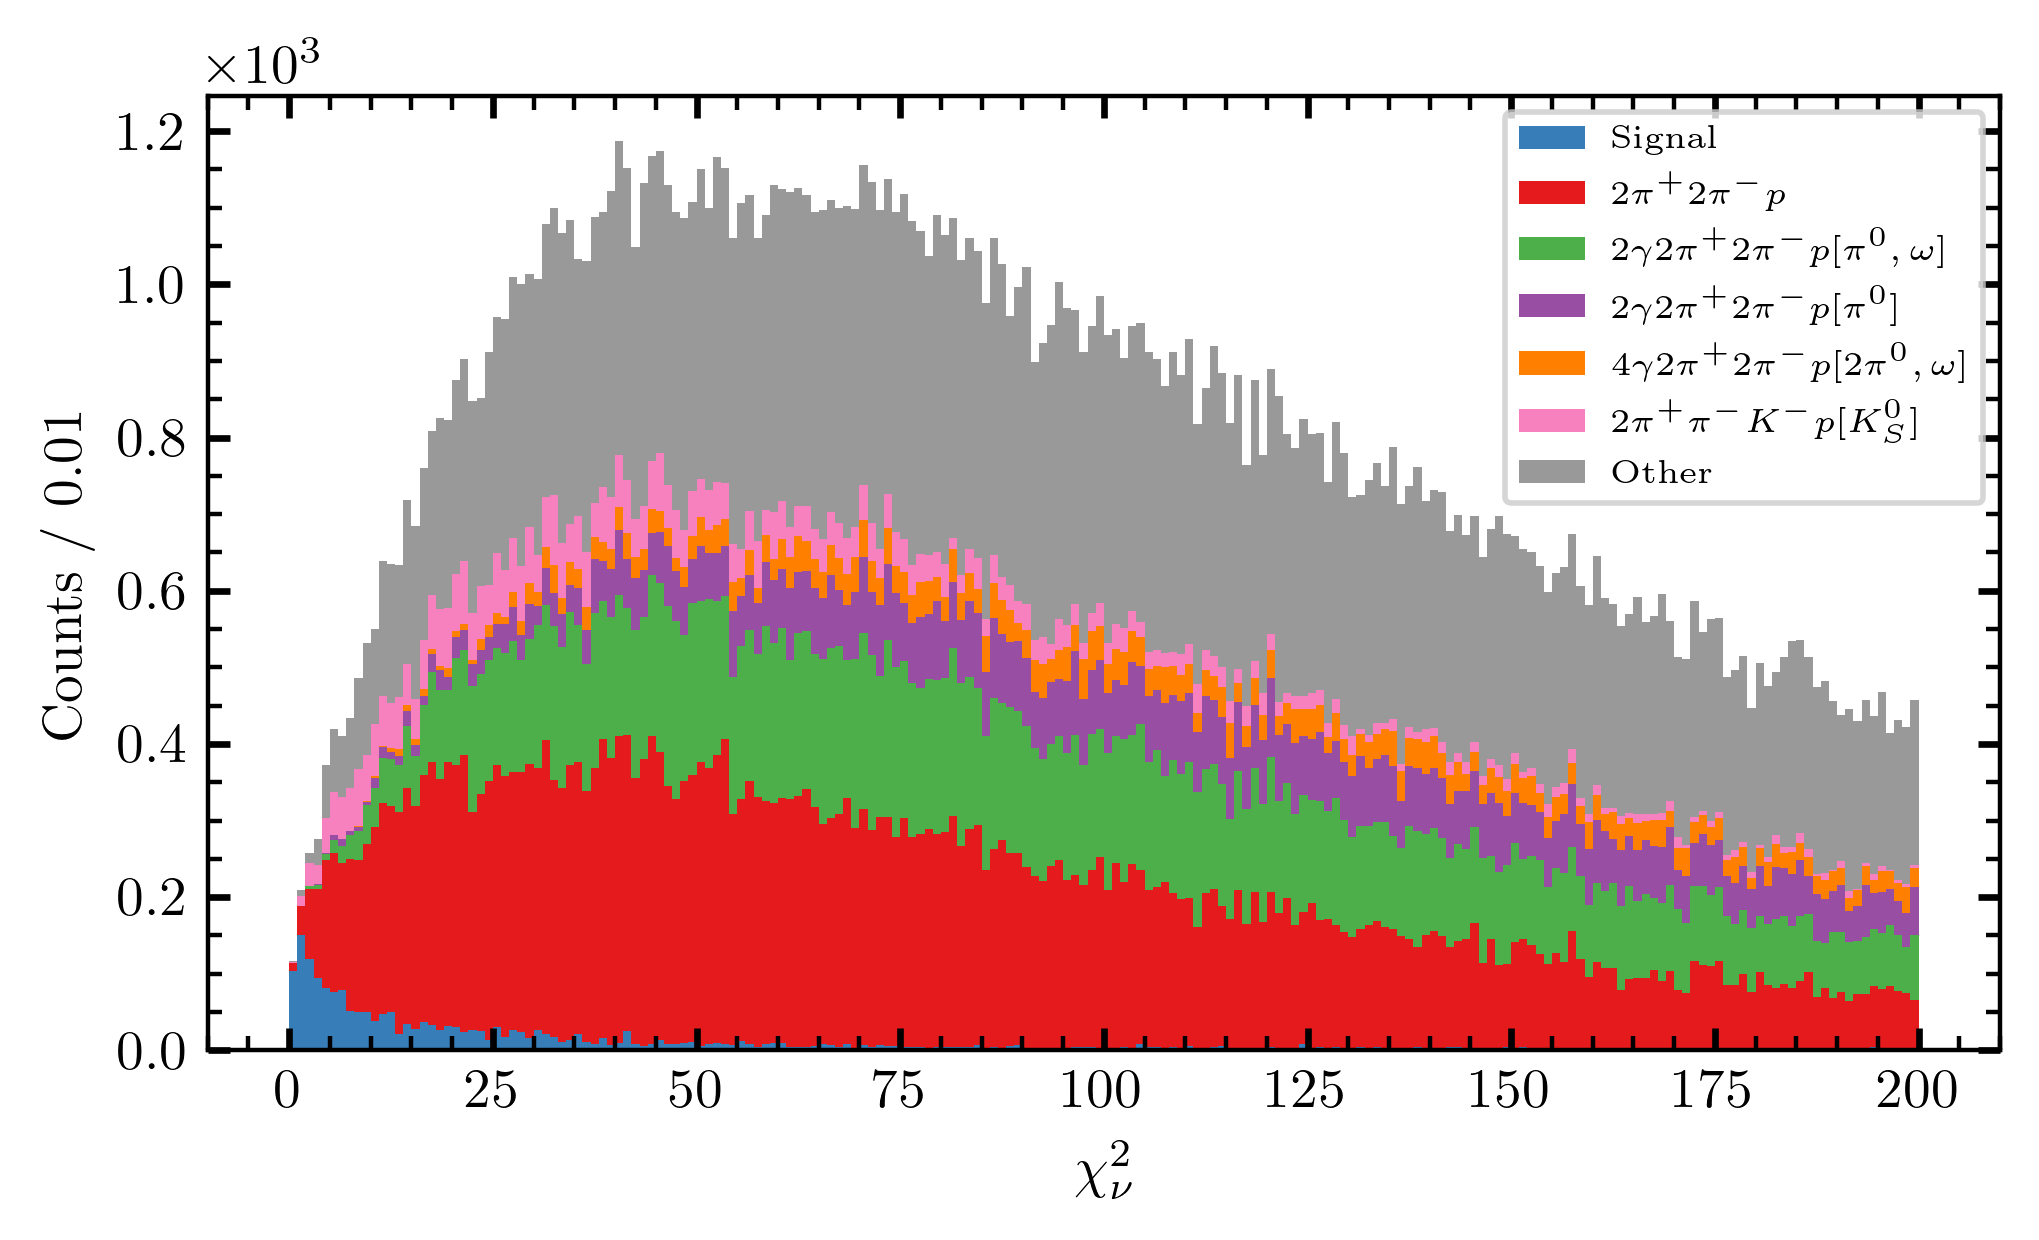
\includegraphics[width=0.8\textwidth]{figures/bggen_chisqdof.png}
  \end{center}
  \caption{The reduced $\chi^2$ statistic of the GlueX kinematic fit for the \texttt{bggen} simulation. The stacked histogram contains the signal channel, $K_S^0K_S^0$ as well as the five most prominent background components.}\label{fig:bggen-chisqdof}
\end{figure}

We will first look at the performance of the GlueX kinematic fit on \texttt{bggen} data in \Cref{fig:bggen-chisqdof}. In this plot, we see the signal, which predictably peaks at $\chi^2_\nu \sim 1$, as well as several background topologies. These topologies are labeled by their final state along with any intermediate decaying resonances in square brackets. The top five potential backgrounds, in order of the size of their contribution after reconstruction, are as follows. First, $2\pi^+2\pi^- p$ shares the final state of the signal channel but does not contain any $K_S^0$ intermediate decays. Second, $2\gamma 2\pi^+ 2\pi^- p [\pi^0, \omega]$ contains an $\omega$ which decays to $\pi^+\pi^-\pi^0$, followed by the $\pi^0$ decaying to $2\gamma$. The addition of extra photons is common in these backgrounds, since missing the photon detections makes the final state identical to the signal. The next two reactions, $2\gamma 2\pi^+ 2\pi^- p [\pi^0]$ and $4\gamma 2\pi^+ 2\pi^- p [2\pi^0, \omega]$ both include an undetected $\pi^0$. Finally, $2\pi^+\pi^- K^- p[K_S^0]$ contains a $K^-$ which is mistakenly identified as a $\pi^-$.

It seems sensible to make a cut on the $\chi^2_\nu$ of the kinematic fit, since the signal is clearly favored at lower values. Below $\chi^2_\nu < 10$, the background topologies are dominated by the $4\pi$ channel which does not contain kaons. As such, this source of background will be our primary focus for removal.

\subsection{Fiducial Cuts}\label{sub:fiducial-cuts}
To get a clearer picture of the data, we will first make a loose cut selecting only events with $\chi^2_\nu < 10$. We can then generate phase-space Monte Carlo for the $4\pi$ background reaction and search for potential ways to separate it from the signal by comparing the distributions of common kinematic variables.

\begin{figure}
  \begin{center}
    \includegraphics[width=0.8\textwidth]{ext/analysis/plots/chisqdof_combined_None_None_None.png}
  \end{center}
  \caption{The normalized distributions of $\chi^2_\nu$ for the true data and phase-space signal and $4\pi$ background Monte Carlo.}\label{fig:data-combined-chisqdof}
\end{figure}

In \Cref{fig:data-combined-chisqdof}, we can see the various distributions of the data and each simulated channel. Unfortunately, the data distribution resembles the $4\pi$ background distribution much better than the signal Monte Carlo, but now we also know that the signal decays rapidly at higher values of $\chi^2_\nu$, so a tighter selection might improve the signal-to-background ratio, even if we cannot immediately see a peak in the data near unity. It is difficult to choose a value at which to cut in this variable, but the choice is largely arbitrary. We will be using a statistical weighting method in \Cref{sec:splot} to subtract the non-strange background represented by the $4\pi$ Monte Carlo, but we must make some choice on $\chi^2_\nu$ before that step in the analysis to reduce other backgrounds mentioned in \Cref{sec:data-selection}. For simplicity, we will conduct the entire analysis using a selection of $\chi^2_\nu < 3.0$, and we will later select several other values on either side of this cut to study its systematic effect in \Cref{sec:systematic-studies}.

As mentioned in \Cref{sec:data-selection}, the asymmetry in missing energy in \Cref{fig:me-combined} likely comes from background channels with photons which were missed in reconstruction. The selection on $\chi^2_\nu$ greatly reduces the contributions from these backgrounds, as can be seen in \Cref{fig:me-combined-chisqdof-3.0}

\begin{figure}
  \begin{center}
    \includegraphics[width=0.8\textwidth]{ext/analysis/plots/me_combined_chisqdof_3.0_None_None_None.png}
  \end{center}
  \caption{Normalized distributions of the missing energy ($E_i - E_f$) for data, phase-space signal Monte Carlo, and $4\pi$ background Monte Carlo after a selection of $\chi^2_\nu < 3.0$ is applied.}\label{fig:me-combined-chisqdof-3.0}
\end{figure}


\begin{figure}
  \begin{center}
    \includegraphics[width=0.8\textwidth]{ext/analysis/plots/mm2_combined_chisqdof_3.0_None_None_None.png}
  \end{center}
  \caption{The normalized distributions of missing mass squared for the true data and phase-space signal and $4\pi$ background Monte Carlo after a selection of $\chi^2_\nu < 3.0$ is applied.}\label{fig:mm2-combined-chisqdof-3.0}
\end{figure}

Another common selection which can be made is on the squared missing mass of an event, which is just the square of the difference between the initial- and final-state four-momenta. This variable, visualized in \Cref{fig:mm2-combined-chisqdof-3.0}, predictably peaks at zero for the data, signal Monte Carlo, and background Monte Carlo, and the overall distributions for the signal and backgound simulated events are nearly identical. This indicates that a selection on this variable would not be very useful at distinguishing the signal from the background.

There are two more minor selections which we will perform on the data. The first is a selection on the invariant mass of $K_S^0K_S^0$ at $\text{IM} < \SI{2.0}{\giga\electronvolt}$. This is done because models we use later to describe the data do not include any higher-mass resonances, and data past this point causes issues with the mass-dependent fits in \Cref{sec:mass-dependent-fits}. The other is a selection on the $z$-vertex of the target proton. We know the exact location of the target with respect to the detector, and we only want to deal with events which we know originated inside this target. The distribution of the $z$-vertex values can be seen in \Cref{fig:protonz-combined}. We will select events with $\SI{50}{\centi\meter} < z < \SI{80}{\centi\meter}$, as this is the known length and position of the target relative to the detector elements. While there is an indication of events in the signal Monte Carlo in the regions which are removed, we know that while these events originated from the target, their $z$-vertex has been misidentified, so we should remove them anyway.


\begin{figure}
  \begin{center}
    \includegraphics[width=0.8\textwidth]{ext/analysis/plots/protonz_combined_None_None_None.png}
  \end{center}
  \caption{The normalized distributions of the target proton $z$-vertex for the true data and phase-space signal and $4\pi$ background Monte Carlo (no cuts applied).}\label{fig:protonz-combined}
\end{figure}

An impetus for studying this channel was originally a search for excited hyperons\textemdash baryons with strange quark content. In particular, $\Sigma^+$ resonances should form in the invariant mass distribution of $K_S^0 p$, where the other kaon is required to conserve strangeness in the strong production of this baryon. There is a symmetry between the identical kaons which must first be accounted for. We could pair either kaon with the proton to form the $\Sigma^+$, but there is a more likely pairing which can be found by first recognizing that the heavier hyperon will generally move more backwards in the center-of-momentum frame than the lighter bachelor $K_S^0$. Therefore, the kaon which is moving in a further backward direction is more likely to correspond with the hyperon decay candidate. We can sort the kaons by their $\cos\theta$ in the center-of-momentum frame and call the more backward-going kaon $K_{S,B}^0$. The invariant mass spectrum of $K_{S,B}^0 p$ can be seen in \Cref{fig:baryon-mass-data-pz-chisqdof-3.0}. The enhancement around $\SI{1.7}{\giga\electronvolt}$ likely corresponds to some combination of the $\Sigma^+(1660)$, $\Sigma^+(1670)$, $\Sigma^+(1750)$, and $\Sigma^+(1775)$ resonances. We do not see much indication of states above $\SI{2}{\giga\electronvolt}$.

\begin{figure}
  \begin{center}
    \includegraphics[width=0.8\textwidth]{ext/analysis/plots/baryon_mass_data_pz_chisqdof_3.0_None_None_None.png}
  \end{center}
  \caption{The mass distribution of the backward-going $K_S^0$ combined with the proton. Only the proton $z$-vertex and $\chi^2_\nu$ cuts are applied, as the cut on invariant mass reduces much of the visible baryon contribution which tends to show up at higher $K_S^0K_S^0$ invariant mass.}\label{fig:baryon-mass-data-pz-chisqdof-3.0}
\end{figure}


This angle also gives us a handle on separating baryonic and mesonic topologies. If we plot the $\cos\theta$ of $K_{S,B}^0$ against the invariant mass of $K_{S,B}^0 p$, as in \Cref{fig:ksb-costheta-v-baryon-mass-data-pz-chisqdof-3.0}, we find a strong and somewhat expected dependence. The majority of the baryonic contribution occurs at angles with $\cos\theta < 0$. Likewise, the mesonic contribution is mostly confined to angles of $\cos\theta > 0$, as seen in figures \Cref{fig:ksb-costheta-v-meson-mass-data-pz-chisqdof-3.0,fig:meson-mass-data-pz-masscut-chisqdof-3.0-mesons}. While it may not be obvious that there even are meson resonances here, we will see their contributions much more clearly after the statistical weighting procedures defined in \Cref{sec:splot} have been applied, after which we will revisit these plots. We will also conduct our analysis without this selection in \Cref{sec:systematic-studies} for completeness. We can also isolate the baryon contributions by reversing this selection, and the result of this is seen in \Cref{fig:baryon-mass-data-pz-masscut-chisqdof-3.0-baryons}.

\begin{figure}
  \begin{center}
    \includegraphics[width=0.8\textwidth]{ext/analysis/plots/ksb_costheta_v_baryon_mass_data_pz_chisqdof_3.0_None_None_None.png}
  \end{center}
  \caption{The center-of-momentum azimuthal angle of $K_{S,B}^0$ plotted against the invariant mass of $K_{S,B}^0 p$. The baryonic contribution occurs mostly at far backward angles, while mesons appear at the far forward angles. Only the proton $z$-vertex and $\chi^2_\nu$ cuts are applied, as the cut on invariant mass reduces much of the visible baryon contribution which tends to show up at higher $K_S^0K_S^0$ invariant mass.}\label{fig:ksb-costheta-v-baryon-mass-data-pz-chisqdof-3.0}
\end{figure}

\begin{figure}
  \begin{center}
    \includegraphics[width=0.8\textwidth]{ext/analysis/plots/ksb_costheta_v_meson_mass_data_pz_chisqdof_3.0_None_None_None.png}
  \end{center}
  \caption{The center-of-momentum azimuthal angle of $K_{S,B}^0$ plotted against the invariant mass of $K_S^0K_S^0$. The baryonic contribution occurs mostly at far backward angles, while mesons appear at the far forward angles. Only the proton $z$-vertex and $\chi^2_\nu$ cuts are applied, as the cut on invariant mass reduces much of the visible baryon contribution which tends to show up at higher $K_S^0K_S^0$ invariant mass.}\label{fig:ksb-costheta-v-meson-mass-data-pz-chisqdof-3.0}
\end{figure}

\begin{figure}
  \begin{center}
    \includegraphics[width=0.8\textwidth]{ext/analysis/plots/meson_mass_data_pz_masscut_chisqdof_3.0_mesons_None_None.png}
  \end{center}
  \caption{The invariant mass of $K_S^0K_S^0$ across all datasets after all fiducial selections are applied.}\label{fig:meson-mass-data-pz-masscut-chisqdof-3.0-mesons}
\end{figure}

\begin{figure}
  \begin{center}
    \includegraphics[width=0.8\textwidth]{ext/analysis/plots/baryon_mass_data_pz_masscut_chisqdof_3.0_baryons_None_None.png}
  \end{center}
  \caption{The invariant mass of $K_S^0K_S^0$ across all datasets after all fiducial selections are applied, but with the baryon rejection cut reversed to select baryons.}\label{fig:baryon-mass-data-pz-masscut-chisqdof-3.0-baryons}
\end{figure}

Finally, we can examine some of the typical detector plots which are used to separate and identify charged particles, namely the energy loss from these charged tracks as measured by the FDC and CDC. As we can see in \Cref{fig:dedx-v-p-cdc-proton-pz-masscut-chisqdof-3.0-mesons,fig:dedx-v-p-cdc-pions-pz-masscut-chisqdof-3.0-mesons}, the data recorded in the CDC after the previous fiducial selections is in agreement with that of the signal Monte Carlo. Next, in the FDC, we do not retain a significant number of proton tracks due to the baryon rejection cut, but enough pions are recorded in the FDC to reveal a discrepancy between data and Monte Carlo, as seen in \Cref{fig:dedx-v-p-fdc-pions-pz-masscut-chisqdof-3.0-mesons}. The signal Monte Carlo here tells us that out of the two horizontal bands, the upper band coincides with real pions, while the other band is likely some background. While the total number of pions which end up in the FDC is small, it is still important to remove these background events, and we will do so with a selection on the energy loss {\color{red}Note to committee, this is a work-in-progress which we do not expect will significantly effect the rest of the thesis}.


\begin{figure}
    \centering
    \begin{subfigure}{0.45\textwidth}
        \includegraphics[width=\linewidth]{ext/analysis/plots/dedx_v_p_cdc_proton_sigmc_pz_masscut_chisqdof_3.0_mesons_None_None.png}
        \caption{Signal Monte Carlo}
    \end{subfigure}
    \hfill
    \begin{subfigure}{0.45\textwidth}
        \includegraphics[width=\linewidth]{ext/analysis/plots/dedx_v_p_cdc_proton_data_pz_masscut_chisqdof_3.0_mesons_None_None.png}
        \caption{Data}
    \end{subfigure}
    \caption{The energy loss in the CDC for protons after all fiducial cuts are applied.}\label{fig:dedx-v-p-cdc-proton-pz-masscut-chisqdof-3.0-mesons}
\end{figure}

\begin{figure}
    \centering
    \begin{subfigure}{0.45\textwidth}
        \includegraphics[width=\linewidth]{ext/analysis/plots/dedx_v_p_cdc_piplus1_sigmc_pz_masscut_chisqdof_3.0_mesons_None_None.png}
        \caption{Signal Monte Carlo}
    \end{subfigure}
    \hfill
    \begin{subfigure}{0.45\textwidth}
        \includegraphics[width=\linewidth]{ext/analysis/plots/dedx_v_p_cdc_piplus1_data_pz_masscut_chisqdof_3.0_mesons_None_None.png}
        \caption{Data}
    \end{subfigure}
    \vspace{1em}
    \begin{subfigure}{0.45\textwidth}
        \includegraphics[width=\linewidth]{ext/analysis/plots/dedx_v_p_cdc_piminus1_sigmc_pz_masscut_chisqdof_3.0_mesons_None_None.png}
        \caption{Signal Monte Carlo}
    \end{subfigure}
    \hfill
    \begin{subfigure}{0.45\textwidth}
        \includegraphics[width=\linewidth]{ext/analysis/plots/dedx_v_p_cdc_piminus1_data_pz_masscut_chisqdof_3.0_mesons_None_None.png}
        \caption{Data}
    \end{subfigure}
    \caption{The energy loss in the CDC for pions after all fiducial cuts are applied.}\label{fig:dedx-v-p-cdc-pions-pz-masscut-chisqdof-3.0-mesons}
\end{figure}

\begin{figure}
    \centering
    \begin{subfigure}{0.45\textwidth}
        \includegraphics[width=\linewidth]{ext/analysis/plots/dedx_v_p_fdc_piplus1_sigmc_pz_masscut_chisqdof_3.0_mesons_None_None.png}
        \caption{Signal Monte Carlo}
    \end{subfigure}
    \hfill
    \begin{subfigure}{0.45\textwidth}
        \includegraphics[width=\linewidth]{ext/analysis/plots/dedx_v_p_fdc_piplus1_data_pz_masscut_chisqdof_3.0_mesons_None_None.png}
        \caption{Data}
    \end{subfigure}
    \vspace{1em}
    \begin{subfigure}{0.45\textwidth}
        \includegraphics[width=\linewidth]{ext/analysis/plots/dedx_v_p_fdc_piminus1_sigmc_pz_masscut_chisqdof_3.0_mesons_None_None.png}
        \caption{Signal Monte Carlo}
    \end{subfigure}
    \hfill
    \begin{subfigure}{0.45\textwidth}
        \includegraphics[width=\linewidth]{ext/analysis/plots/dedx_v_p_fdc_piminus1_data_pz_masscut_chisqdof_3.0_mesons_None_None.png}
        \caption{Data}
    \end{subfigure}
    \caption{The energy loss in the FDC for pions after all fiducial cuts are applied. {\color{red}Note to committee: The extra structure here will be addressed with a cut, but it will have minimial impact on this thesis and take several days to reprocess data. Expect an update to this section.}}\label{fig:dedx-v-p-fdc-pions-pz-masscut-chisqdof-3.0-mesons}
\end{figure}

In total, we have the fiducial selections on the data illustrated in \Cref{tab:fiducial-cuts}.

\begin{table}
  \begin{center}
    \begin{tabular}{cc}\toprule
      Variable & Selected Values \\\midrule
      $\chi^2_\nu$ & $\chi^2_\nu < 3.0$ \\
      Mass of $K_S^0K_S^0$ & $ m < \SI{2.0}{\giga\electronvolt} $ \\
      Target proton-$z$ & $\SI{50}{\centi\meter} < z < \SI{80}{\centi\meter}$ \\
      $\cos\theta_{\text{CM}}$ of $K_{S,B}^0$ & $ \cos\theta_{\text{CM}} > 0.0 $ \\\bottomrule
    \end{tabular}
    \caption{Fiducial cuts performed after event reconstruction.}\label{tab:fiducial-cuts}
  \end{center}
\end{table}

\subsection{Accidental Subtraction}\label{sub:accidental-subtraction}
\section{sPlot Weighting}\label{sec:splot}
At this stage in the analysis, we have no more simple cuts which can improve the signal-to-background ratio in the dataset, but we know there must still be background remaining, as is indicated by the excess events with small kaon rest-frame lifetimes seen in \Cref{fig:rfl-pre-splot}. In this figure, we see that one of the intrinsic properties of a $K_S^0$, its well-known lifetime around $\SI{89.54}{\pico\second}$, is not present in the data. Rather, we seem to have at least two exponential slopes in the rest-frame lifetime distribution of each kaon, one which is close to what we see in signal Monte Carlo, and another which is similar to the $4\pi$ background Monte Carlo. The $K_S^0$ lifetime comes from the fact that it contains a strange quark but decays to two non-strange mesons, and a weak interaction is required for this to occur. While we might not know the exact process which creates the $4\pi$ background, we can assume a strong interaction produces the pions, which should happen several orders of magnitude faster than the $K_S^0$ decay. Due to the resolution of the detector, we still expect these events to appear to have some non-zero distribution in rest-frame lifetime when we mistakenly interpret pairs of pions as kaons, but it will be vastly different from that of the signal. Rather than cut out the low-lifetime events (greatly reducing the $K_S^0$ signal which also peaks at zero), we now turn to a more elaborate method of separating the signal from this potential background influence called sPlot~\cite{Pivk2005}\footnote{This is stylized as ${}_s\mathcal{P}lot$ in the original paper, but I find this tedious to type and to read.}, a weighting scheme which roughly weights each event by the probability of it coming from the signal or background distribution. However, na\"ively weighting by probability (a method dubbed ``inPlot'') can cause issues which can fortunately be easily corrected. We begin by giving a basic explanation of inPlot before describing the sPlot correction.

\begin{figure}
  \begin{center}
      \includesvg[width=0.8\linewidth]{ext/analysis/plots/rfl_combined_pz_masscut_chisqdof_3.0_mesons_None_None.svg}
  \end{center}
  \caption{The rest-frame lifetime of kaons in data, signal Monte Carlo, and background Monte Carlo. The data distribution clearly contains two exponential slopes: a peak which resembles the $4\pi$ Monte Carlo distribution, and a tail of true $K_S^0$s which resembles the signal Monte Carlo.}\label{fig:rfl-pre-splot}
\end{figure}

For all of the statistical weighting methods which will be mentioned here, we need some model for the signal and background probability distribution functions (PDFs) for some ``discriminating'' variable. This variable is called ``discriminating'' because it the variable for which we know the shape of these distributions beforehand. The usual example is a ``bump-on-a-background'', in which the discriminating variable may be a mass distribution ($m$) where signal events show up as a peaking structure while background events are more uniformly distributed. In such situations, it is common to use the extremes of the mass distribution (sidebands) as estimates of the background everywhere, weighting these events negatively while the events in the peak are weighted positively (a sideband subtraction). Rather than specifying peak and sideband regions, we can fit the mass distribution to some mixture of a signal (peak) PDF $f_S(m)$ and a background (flat) PDF $f_B(m)$. From such a fit, we obtain estimated number of signal ($N_S$) and background ($N_B$) events in our dataset (and possibly some shape parameters for the signal and background PDFs). We could then assign weights to each event as in \Cref{eq:inplot-weights-mass},

\begin{equation}
  w(m) = \frac{N_S f_S(m)}{N_S f_S(m) + N_B f_B(m)},
  \label{eq:inplot-weights-mass}
\end{equation}

We might want to look at the ``signal'' inPlots for the decay angles $\theta$ and $\varphi$ (control variables) in the helicity system after calculating the inPlot weights from a fit to the mass distribution (discriminating variable). However, as shown by Pivk and Le Diberder~\cite{Pivk2005}, we can only use inPlot in cases where the control variables are statistically dependent on the discriminating variable\footnote{In practice, more than one discriminating variable can be used.}, $y$. In other words, our example would only be valid if $\theta = \theta(m)$ and $\phi = \phi(m)$. For the time being, let us assume that this is not the case, and that we wish to use the distribution of some variable which is statistically independent from the variables we are plotting and analyzing\footnote{Total statistical (in)dependence is a very strict requirement, but we will later see that small modifications to the sPlot method can permit amounts of dependence between the two extremes.}. A correction term can be applied to give us the sPlot version of \Cref{eq:inplot-weights-mass},

\begin{equation}
  w(y) = \tilde{w}(y)\frac{V_{SS}f_S(y) + V_{SB}f_B(y)}{N_S f_S(y) + N_B f_B(y)},\quad \text{where } V^{-1}_{ij} = \sum_{y} \frac{\tilde{w}(y)f_i(y)f_j(y)}{\left(N_S f_S(y) + N_B f_B(y)\right)^2},
  \label{eq:splot-weights}
\end{equation}
where $y$ represents any set of discriminating variables (not necessarily a mass), and $\tilde{w}(y)$ is any pre-existing weight associated with the event (weights from accidental subtraction, for instance). The $V^{-1}$ matrix can also be understood as the covariance matrix between the free parameters $N_S$ and $N_B$ in the fit of the signal-background mixture, $V^{-1}_{ij} = -N\pdv[2]{\ln\mathcal{L}}{N_i}{N_j}$, although there is reason to believe that direct calculation by inverting the Hessian matrix from the fit will lead to less accurate results than the manual calculation method given in \Cref{eq:splot-weights}~\cite{Dembinski2022}.

Now that we have a method of assigning weights, we must pick the discriminating variables. As mentioned, these weighting methods work well on the classic ``bump-on-a-background'' distributions because it is easy to identify the signal and background PDFs, but because the mass of the kaons is constrained in the kinematic fit, the fitted mass of each kaon is just a $\delta$-function and combination of measured masses for each $\pi^+\pi^-$ pair will yield a Normal distribution with little to no apparent background (by construction), so we must be a bit more clever in selecting discriminating variables. By examining the \texttt{bggen} analysis done in \Cref{sec:data-selection}, we can see that most likely sources of background arise when the intermediate kaons are absent from the reaction: $\gamma p \to 4\pi p$. This reaction has the $K_SK_S$ final state, so pairs of pions which reconstruct close enough to kaons will be almost indistinguishable in the data. However, they differ in one key way, namely that the $K_S$ intermediate contains a strange quark while the $\pi^+\pi^-$ decay state does not, so such a decay must occur via the weak interaction, which is notably slower than the strong interaction which would produce pion pairs with no intermediate kaon. In other words, while the signal's rest-frame lifetime distribution should have an exponential slope near the $K_S$ lifetime, the background would theoretically have nearly zero rest-frame lifetime for every event, or a much smaller exponential slope in practice\footnote{An exponential distribution is just what fits the rest-frame lifetime distribution in the $4\pi$ Monte Carlo best and has no other physical implication.}.

Therefore, we will begin by generating both a signal and background dataset in Monte Carlo. We then interpret both datasets as if they were our desired channel by running them through the GlueX reconstruction and reaction filter, as well as all of our selections up to this point. The signal Monte Carlo distribution in \Cref{fig:rfl-pre-splot} mostly follows an exponential distribution, but it flattens out near zero. Rather than use an exponential model, we will use the shape of this distribution itself, as it includes acceptance effects from the detector. The background distribution is roughly exponential, so we will fit the background Monte Carlo to an exponential distribution,

\begin{equation}
  f(t; \lambda) = \lambda \exp{-\lambda t},
  \label{eq:splot-exponential}
\end{equation}
where $\lambda \equiv 1/\tau$, the lifetime of the (hypothesized) kaon in question. To account for the fact that there could be backgrounds other than the one we simulated, we will allow the slope of this background distribution to vary, although we will start the fit at a value obtained from the Monte Carlo simulation. Since we have two independently decaying kaons, we should really form a joint distribution for both, where we will assume each kaon has the same average lifetime:
\begin{equation}
  f(t_1, t_2; \lambda) = \lambda^2 \exp{-\lambda t_1}\exp{-\lambda t_2}
  \label{eq:splot-exponential_joint}
\end{equation}

As mentioned previously, rather than model the signal distribution analytically, we will instead use the distribution from the Monte Carlo itself as the model by binning the simulated data (a bin width of $\SI{1}{\pico\second}$ seems to give a distribution that is decently smooth in practice). In the following discussions, we will use this binned distribution as the model for the signal component and the exponential distribution in \Cref{eq:splot-exponential_joint} for the background component. Because of this, the signal distribution does not have a slope parameter, so we construct a mixture equation which looks like,

\begin{equation}
  g(t_1, t_2; z, \lambda_B) \equiv z \tilde{f}(t_1, t_2) + (1-z) f(t_1, t_2; \lambda_B),
  \label{eq:splot-mixture}
\end{equation}
where $\tilde{f}$ represents the binned distribution, and $z$ is the signal fraction ($N_S = z\cdot N$ and $N_B = (1-z)\cdot N$ where $N_S$ is the number of signal events, $N_B$ is the number of background events, and $N = N_S + N_B$ is the total number of events), and the equation for the likelihood is,

\begin{equation}
  -2\ln\mathcal{L}(z,  \lambda_B) = -2\sum_i^N \tilde{w}_i \ln g(t_{1,i}, t_{2,i}; z, \lambda_B)
  \label{eq:splot-nll}
\end{equation}

\subsection{Non-Factorizing sPlot}\label{sec:non-factorizing-splot}

Over the course of the previous discussion, it was assumed that the discriminating variables, $t_1$ and $t_2$, were statistically independent from the control variables we wish to use in later analyses. The set of control variables must include all variables we use as inputs to the partial-wave analysis in \Cref{ch:partial-wave-analysis}, including the invariant mass $m$ of the $K_S^0K_S^0$ system and the helicity angles $\theta$ and $\varphi$ of the decay. We should now confirm that the rest-frame lifetimes are statistically independent from these control variables (in other words, show that they are statistically independent). To test for statistical independence between $t_{1,2}$ and a given control variable, we first split our dataset into $M$ evenly-spaced quantiles in that control variable, which ensures each bin gets roughly the same number of events. Next, we calculate the likelihood of a null hypothesis which assumes the variables are statistically independent by fitting all datasets simultaneously with a shared $\lambda_B$ parameter. We then calculate the likelihood of an alternative hypothesis, which assumes statistical dependence, by finding the joint likelihood of independent fits of $\lambda_B$ over each quantile. The result of these fits can be formulated as a likelihood ratio,

\begin{equation}
  \Lambda = -2\ln\frac{\sup \mathcal{L}_{H_0}}{\sup \mathcal{L}_{H_1}} = -2\ln\frac{\sup \prod_i^M \mathcal{L}_i(z_i, \lambda_B)}{\sup \prod_i^M \mathcal{L}_i(z_i, \lambda_{B,i})},
  \label{eq:independence-test}
\end{equation}
where $\mathcal{L}_{H_0}$ and $\mathcal{L}_{H_1}$ are the likelihoods of the null and alternative hypotheses respectively, the supremum indicates we are maximizing these likelihoods (in a maximum likelihood fit), the product $\prod_i^M$ iterates over each quantile of data in the given control variable, and $\mathcal{L}_i$ is the likelihood evaluated over data in the $i$th quantile. $\Lambda$ is $\chi^2$ distributed with $M - 1$ degrees of freedom (the difference between $M + 1$ free parameters in the null hypothesis, a signal fraction $z_i$ for each quantile plus the exponential background slope shared across all quantiles, and $2M$ in the alternative hypothesis, a signal fraction and one exponential slope for each quantile). The factor of $2$ is required because $\ln\mathcal{L}(\theta_1,...,\theta_i) \sim -\frac{1}{2}\chi^2_i$ asymptotically with sample size, according to Wilks' theorem. We can obtain a $p$-value representing the likelihood of the null hypothesis being true by evaluating the $p$-value:

\begin{equation}
  p = 1 - F_{\chi^2_{M-1}}(\Lambda),
  \label{eq:significance-test}
\end{equation}
where $F_{\chi^2_{M-1}}(\Lambda)$ is the cumulative distribution function of a $\chi^2$ distribution with $M-1$ degrees of freedom. Following this procedure for the invariant mass of $K_S^0K_S^0$\footnote{No significant statistical dependence was found for the helicity angles.}, we obtain $p$-values of $<2.23\times10^{-308}$ with two, three, or four quantiles. The calculated $p$-values imply that we should reject the null hypothesis and accept that the discriminating (rest-frame lifetime) and control (invariant mass of $K_S^0K_S^0$) variables are not statistically independent. This means we cannot use a traditional sPlot to weight our data.

The results of these tests over the data consistently return $p$-values close to zero (below machine precision). While this may seem surprising, the results are visualized for four quantiles in \Cref{fig:factorization}, and we can see that there is a strong statistcal dependence between the control and discriminating variables which lead to this low $p$-value. Again, the significantly small $p$-values justify the use of non-factorizing sPlot across the background component, meaning that we need at least two background components in the final sPlot weighting\footnote{We found that a similar analysis an exponential signal distribution also indicates a significant amount of non-factorization, but the difference in the slopes of each component are too small to give significantly different fits to the true data. Additionally, we could choose to use the Monte Carlo distribution for the background as well, but that would assume that we have correctly modeled the entire background, while we really only modeled what we believe was the most prominent component.}.

The process for obtaining the correct weights is straightforward, we simply allow for more than one signal and background component in the fit and sum over all signal components when we calculate the final weight values~\cite{Dembinski2022}. Since the weights corresponding to each signal component in the sPlot can be added to each other to obtain a joint weight~\cite{Pivk2005}, \Cref{eq:splot-weights} can be extended to allow multiple signal and background components:

\begin{equation}
  w(y) = \frac{\sum_{j} V_{Sj}f_j(y)}{\sum_{k}N_kf_k(y)},\quad \text{where } V_{ij}^{-1} = \sum_{y} \frac{f_i(y)f_j(y)}{\left(\sum_{k} N_kf_k(y)\right)^2}
  \label{eq:splot-weights-factorizing}
\end{equation}

and $S$ is the index of the signal component.


\begin{figure}
  \begin{center}
    \includesvg[width=0.8\textwidth]{ext/analysis/plots/factorization_fit_pz_masscut_chisqdof_3.0_mesons_10.svg}
  \end{center}
  \caption{Background exponential slopes from fits over four quantiles in $m(K_S^0K_S^0)$ ($x$-axis) of the rest-frame lifetime distributions of data. Both show a definite statistical dependence between rest-frame lifetime and the invariant mass of $K_S^0K_S^0$ with a p-value smaller than machine precision ($p < 2.23 \times 10^{-308}$).}\label{fig:factorization}
\end{figure}

\subsection{Application of Weights}\label{sec:application-of-weights}

The only thing left to do is determine how many background components we should use in the weighting procedure. To this end, we now turn to the Monte Carlo simulations of the $4\pi$-background. By choosing a number of quantiles in invariant mass corresponding to the number of components, we can fit single exponential distributions to each quantile in the simulated background. For instance, if we chose to use three background components, we would divide the background Monte Carlo into three, and fit each quantile to an exponential distribution to obtain a set of three $\lambda_B$ values. The resulting  $\lambda_B$ values could then be used as a starting point for a multi-component fit to the data. Alternatively, the background slopes could be fixed to the values from the fits to simulations, and only the yields would be allowed to float in the fit to data. We will examine two types of models, one where the fit parameters ($\lambda_B$) from Monte Carlo are free and one where they are fixed to values found in fits to the background Monte Carlo (the fit fraction $z$ is free in both cases). To select a model, we can use the relative Akaike Information Criterion (AIC)~\cite{Akaike1998} and the relative Bayesian Information Criterion (BIC)~\cite{Schwarz1978}:
\begin{alignat}{2}
  r\text{AIC} &\equiv \text{AIC} - \text{AIC}_\text{min} \quad\text{where } \text{AIC} &&\equiv 2k - 2\ln\mathcal{L} \\
  r\text{BIC} &\equiv \text{BIC} - \text{BIC}_\text{min} \quad\text{where } \text{BIC} &&\equiv k\ln{N} - 2\ln\mathcal{L},
  \label{eq:information-criteria}
\end{alignat}
where $k$ is the number of free parameters and $N$ is the number of events in the dataset. The optimal model will minimize these criteria. In \Cref{tab:splot-model-results}, all of the relative AIC and BIC values are shown. Since the procedure requires us to minimize $r\text{AIC}$ and $r\text{BIC}$, we find that the model with eight free-floating background slopes should be selected. However, upon plotting the fit result in \Cref{fig:splot-fits}, it is clear that eight slopes are not needed to properly describe the data, despite having the best information criteria. Instead, we will use a model with two free-floating background slopes. It is interesting to note that all of the models where the background slopes were fixed to values obtained from fits over background Monte Carlo are generally much poorer fits overall, despite having fewer degrees of freedom. This possibly reflects the fact that we only modeled one source of background in the Monte Carlo, while many sources could be present in the data.

\input{ext/analysis/reports/splot_report_pz_masscut_chisqdof_3.0_mesons_max_nspec_10.tex}

\input{ext/analysis/reports/splot_fit_pz_masscut_chisqdof_3.0_mesons_free_2.tex}
\input{ext/analysis/reports/splot_fit_pz_masscut_chisqdof_3.0_mesons_free_8.tex}
% TODO: use num2words on the caption here and add a label

\begin{figure}
  \begin{center}
    \begin{subfigure}[t]{\textwidth}
        \begin{center}
          \includesvg[width=.8\columnwidth]{ext/analysis/plots/splot_fit_pz_masscut_chisqdof_3.0_mesons_free_8.svg}
        \caption{The fit to data using a model with eight free-floating background slopes.}
        \end{center}
        \end{subfigure}
        \begin{subfigure}[t]{\textwidth}
          \begin{center}
            \includesvg[width=.8\columnwidth]{ext/analysis/plots/splot_fit_pz_masscut_chisqdof_3.0_mesons_free_2.svg}
        \caption{The fit to data using a model with two free-floating background slopes.}
          \end{center}
        \end{subfigure}
        \caption{Fits of \Cref{eq:splot-mixture} to data using (a) eight and (b) two free-floating background slopes. While the model with eight slopes is better according to information criteria, most of the background slopes are nearly identical to each other, and only two main slopes are present. Because of this, we will use the simpler two-slope model.}\label{fig:splot-fits}
\end{center}
\end{figure}

Before we perform a partial-wave analysis, we will take inventory of the dataset after this weighting proceedure is applied. The current state of the data after all fiducial selections and sPlot weights can be see in ....

\begin{figure}
  \begin{center}
    \includesvg[width=0.8\textwidth]{ext/analysis/plots/meson_mass_data_pz_masscut_chisqdof_3.0_mesons_free_2.svg}
  \end{center}
  \caption{The invariant mass of $K_S^0K_S^0$ after all selections and weights are applied.}\label{fig:meson-mass-data-pz-masscut-chisqdof-3.0-mesons-free-2}
\end{figure}
\begin{figure}
  \begin{center}
    \includesvg[width=0.8\textwidth]{ext/analysis/plots/beam_energy_data_pz_masscut_chisqdof_3.0_mesons_free_2.svg}
  \end{center}
  \caption{The beam energy distribution all selections and weights are applied. The large discontinuities at $\SI{8.2}{\giga\electronvolt}$ and $\SI{8.6}{\giga\electronvolt}$ are due to the difference in the coherent peak range between the Phase-I and Phase-II datasets (see \Cref{tab:run-info}).}\label{fig:beam-energy-data-pz-masscut-chisqdof-3.0-mesons-free-2}
\end{figure}
\begin{figure}
  \begin{center}
    \includesvg[width=0.8\textwidth]{ext/analysis/plots/costheta_hx_v_meson_mass_data_pz_masscut_chisqdof_3.0_mesons_free_2.svg}
  \end{center}
  \caption{The distribution of the azimuthal decay angle of $X \to K_S^0K_S^0$ in the helicity frame after all selections and weights are applied.}\label{fig:costheta-hx-v-meson-mass-data-pz-masscut-chisqdof-3.0-mesons-free-2}
\end{figure}
\begin{figure}
  \begin{center}
    \includesvg[width=0.8\textwidth]{ext/analysis/plots/phi_hx_v_meson_mass_data_pz_masscut_chisqdof_3.0_mesons_free_2.svg}
  \end{center}
  \caption{The distribution of the polar decay angle of $X \to K_S^0K_S^0$ in the helicity frame after all selections and weights are applied.}\label{fig:phi-hx-v-meson-mass-data-pz-masscut-chisqdof-3.0-mesons-free-2}
\end{figure}

\subsection{Neutral Kaon Decay Channels}\label{sub:neutral-kaon-decay-channels}

\chapter{Partial-Wave Analysis}\label{ch:partial-wave-analysis}
\section{Amplitude Formalism}

Now we embark on the topic of amplitudes. We wish to describe the dynamics of our reaction in a way that allows us to extract quantum numbers like spin from our data. There are several difficulties in doing so: First, we are trying to determine the properties of many particles at once, and we know that many resonances in this channel overlap in mass space. This precludes the use of a simple Breit-Wigner description of most of these resonances, as overlapping Breit-Wigners do not preserve unitarity. Second, the GlueX experiment uses a linearly polarized photon beam, so it behooves us to use a formalism which can include this polarization. Finally, there are many resonances in this channel, and while we have the largest photoproduction dataset to date, we are still relatively data limited, which further complicates any dynamical description. The majority of this section is a summary of the formalisms described in \cite{chung_spin_1971} and \cite{richman_experimenters_1984}.

\subsection{Single-Particle Helicity States}

We begin by defining a set of observables which are independent of frames and rotations on those frames. This is known as the helicity formalism, where helicity resembles the spin projection along the axis of a particle's motion. First, we define a rotation $R(\alpha, \omega, \gamma)$ as a matrix whose action on a vector is a rotation about the Euler angles $\alpha$, $\omega$, and $\gamma$. For each rotation, we can define a unitary operator $U[R]$ which has the group property $U[R_2 R_1] = U[R_2] U[R_1]$ as it is an operator on the group $SO(3)$. Being an operator on $SO(3)$, we can also write it as

\begin{equation}
  U[R(\alpha,\omega,\gamma)] = e^{-\imath \alpha J_z} e^{-\imath \omega J_y} e^{-\imath \gamma J_z}
  \label{eq:rotation-rep}
\end{equation}

We can then describe the matrix elements of this operator in the angular momentum eigenbasis $\ket{jm}$ (representing a spin-$j$ particle where $m$ is the projection of spin onto the $\hat{z}$-axis) with the Wigner D-matrix:

\begin{gather}
  U[R(\alpha, \omega, \gamma)] \equiv \sum_{m'} \ket{jm} D_{m'm}^j(R(\alpha, \omega, \gamma)) \\
  \text{where} \notag\\
  D_{m'm}^j(\alpha, \omega, \gamma) \equiv e^{-\imath m' \alpha} d_{m'm}^j e^{-\imath m\gamma} \\
  \text{and} \notag\\
  d_{m'm}^j(\omega) = \mel{jm'}{e^{-\imath\omega J_y}}{jm}
  \label{eq:wigner-d-definition}
\end{gather}

We can further extend this eigenbasis to include linear momentum by introducing Lorentz boosts $L(\vec{\beta})$. We denote the operation of a boost along the $\hat{z}$-axis with velocity $\beta$ as $L_z(\beta)$. A boost in any direction described by polar angles $(\theta, \varphi)$ can be achieved by rotating the $\hat{z}$-axis to align with the direction vector, boosting in the new $\hat{z}$-direction, and rotating back:

\begin{equation}
  L(\vec{\beta}) = R(\varphi, \theta, 0) L_z(\beta) R^{-1}(\varphi,\theta,0)
\end{equation}

Together, the space of rotations and boosts defines the Lorentz group, where each arbitrary Lorentz transformation $\Lambda$ has a unitary operator $U[\Lambda]$ with the group property $U[\Lambda_2 \Lambda_1] = U[\Lambda_2]U[\Lambda_1]$, so in terms of operators, we can also write

\begin{equation}
  U[L(\vec{p})] = U[R(\varphi, \theta, 0)]U[L_z(p)]U^{-1}[R(\varphi,\theta,0)]
\end{equation}

Finally, this allows us to define the ``canonical'' basis for a single particle as
\begin{equation}
  U[L(\vec{p})]\ket{jm} \equiv \ket{\vec{p},jm}
  \label{eq:canonical-single-particle}
\end{equation}

Unfortunately, the quantum number $m$ is only valid in the rest frame of the state because the $\hat{z}$-axis of the rest frame is not equivalent to the $\hat{z}$-axis in any arbitrarily Lorentz-transformed frame. Therefore, we will define helicity $\lambda$ as the projection of spin along the direction of motion and introduce new helicity states,

\begin{equation}
  \ket{\vec{p},j\lambda} = U[L(\vec{p})]U[R(\varphi,\theta,0)]\ket{j\lambda} = U[R(\varphi,\theta,0)]U[L_z(p)]\ket{j\lambda}
  \label{eq:helicity-single-particle}
\end{equation}

In this definition, we have two ways of obtaining the helicity frame: We can either rotate the state first such that the quantization axis is aligned with $\vec{p}$ and then boost in the $\hat{p}$-direction or we can first boost in the $\hat{z}$-direction and then rotate. In either equivalent case, $\lambda$ is invariant under rotations as well as boosts parallel to $\vec{p}$. Finally, we can define these helicity states over a basis of canonical states:

\begin{equation}
  \ket{\vec{p},j\lambda} = \sum_m D_{m\lambda}^j(R(\varphi, \theta, 0)) \ket{\vec{p}, jm}
  \label{eq:canonical-to-helicity}
\end{equation}

The single-particle states are normalized such that

\begin{gather}
  \bra{\vec{p}',j'\lambda'}\ket{\vec{p},j\lambda} = \tilde{\delta}(\vec{p}' - \vec{p})\delta_{j'j}\delta_{\lambda'\lambda} \\
  \text{with } \tilde{\delta}(\vec{p}' - \vec{p}) = (2\pi)^3(2E)\delta^{(3)}(\vec{p}'-\vec{p}) \notag
  \label{eq:helicity-normalization}
\end{gather}

since the Lorentz-invariant phase space element is given by $\tilde{\dd{p}} = \frac{\dd[3]{\vec{p}}}{(2\pi)^3(2E)}$. This gives the following representation of the identity:

\begin{equation}
  \sum_{j\lambda}\int \ket{\vec{p},j\lambda}\tilde{\dd{p}}\bra{\vec{p},j\lambda} = I
\end{equation}

\subsection{Two-Particle Helicity States}

Of course, we would like to extend these states to be able to talk about interactions and decays. For notation, I will use $\Omega$ to represent the polar angles $\theta$ and $\varphi$ and $\varnothing$ to describe the specific value of $0$ for both of these angles. Similarly, $R_\Omega$ and $R_\varnothing$ will represent the corresponding rotation operators (the second being a null rotation the direction of the $\hat{z}$-axis). $R$ without subscript or angles will represent an arbitrary rotation whose angles are not important for the derivation.

Next, we can define a joint state of two particles with masses $w_1$ and $w_2$ (to avoid confusion with angular moments) and spins $s_1$ and $s_2$. In the center-of-momentum (COM) frame, these particles are back-to-back, and we can define the momentum of particle 1 as $\vec{p}$ with direction $\Omega$ and particle 2 as $-\vec{p}$. Then the joint canonical state, up to a normalization constant $\mathcal{N}$, is given by

\begin{equation}
  \ket{\Omega,s_1m_1s_2m_2} = \mathcal{N} U[L(\vec{p})]\ket{s_1m_1} U[L(-\vec{p})]\ket{s_2m_2}
  \label{eq:two-particle-canonical}
\end{equation}

Such a state can also be described with a total spin $s$ and moment $m_s$:

\begin{equation}
  \ket{\Omega, sm_s} = \sum_{m_1m_2} \left(s_1m_1s_2m_2\mid sm_s\right)\ket{\Omega,s_1m_1s_2m_2}
\end{equation}

Here, $\left(s_1m_1s_2m_2\mid sm_s\right)$ is the Clebsch-Gordan coefficient describing the angular momentum coupling. Next, we can add additional angular momentum apart from the spin. For a system with angular momentum $\ell$ with moment $m$, we use the fact that $\bra{\Omega}\ket{\ell m} = Y_{\ell}^m(\Omega)$ (spherical harmonics) to define

\begin{equation}
  \ket{\ell m s m_s} = \int \dd{\Omega} Y_{\ell}^m(\Omega) \ket{\Omega; s m_s}
  \label{eq:two-particle-canonical-angular-momentum}
\end{equation}

Next, the spin $s$ and angular momentum $\ell$ can be coupled into the total angular momentum $J$ with moment $M$:

\begin{equation}
  \ket{J M \ell m s m_s} = \sum_{m\,m_s} \left(\ell m s m_s \mid JM\right)\ket{\ell m s m_s}
  \label{eq:two-particle-canonical-total-angular-momentum}
\end{equation}

This coupled state is still in the canonical formalism, and we would like to use the helicity basis. Using \Cref{eq:helicity-single-particle},

\begin{equation}
  \ket{\Omega,s_1\lambda_1 s_2\lambda_2} = \mathcal{N} U[R_\Omega] \underbrace{\left(U[L_z(p)]\ket{s_1\lambda_1} U[L_{-z}(p)]\ket{s_2,-\lambda_2}\right)}_{\ket{\varnothing, s_1\lambda_1 s_2\lambda_2}}
  \label{eq:two-particle-helicity}
\end{equation}

To obtain states with a total angular momentum, we can integrate over the space of all rotations, weighted by Wigner D-matrices:

\begin{equation}
  \ket{JM s_1\lambda_1 s_2\lambda_2} = \frac{N_J}{2\pi} \int \dd{R} D_{M\mu}^{J*}(R) U[R]\ket{\varnothing, s_1\lambda_1 s_2\lambda_2}
\end{equation}

This is, of course, incomplete, as we have not defined the normalization factor $N_J$ or the coupling $\mu$ which relates helicities to total angular momentum. To do both, let us specify the rotation $R$ as follows,

\begin{align}
  \ket{JM s_1\lambda_1 s_2\lambda_2} &= \frac{N_J}{2\pi}\int \dd{R} D_{M\mu}^{J*}(R) U[R(\varphi, \theta, \gamma)]\ket{\varnothing, s_1\lambda_1 s_2\lambda_2} \notag \\
                                     &= \frac{N_J}{2\pi}\int \dd{R} D_{M\mu}^{J*}(R) U[R(\varphi, \theta, 0)]U[R(0, 0, \gamma)]\ket{\varnothing, s_1\lambda_1 s_2\lambda_2} \notag \\
                                     &= \frac{N_J}{2\pi}\int \dd{R} D_{M\mu}^{J*}(R) e^{-\imath (\lambda_1 - \lambda_2)\gamma}U[R(\varphi, \theta, 0)]\ket{\varnothing, s_1\lambda_1 s_2\lambda_2} \notag \\
                                     &= \frac{N_J}{2\pi}\int \dd{\Omega}\dd{\gamma} e^{\imath M \varphi} d^{J*}_{M\mu} e^{\imath \mu \gamma} e^{-\imath (\lambda_1 - \lambda_2)\gamma}U[R(\varphi, \theta, 0)]\ket{\varnothing, s_1\lambda_1 s_2\lambda_2} \notag \\
                                     &= \frac{N_J}{2\pi}\int \dd{\Omega}\dd{\gamma} e^{\imath M \varphi} d^{J*}_{M\mu} e^{\imath (\mu - (\lambda_1 - \lambda_2)) \gamma} \ket{\Omega, s_1\lambda_1 s_2\lambda_2} \notag \\
                                     &= N_J\int \dd{\Omega} D_{M\lambda}^{J*}(R_{\Omega}) \ket{\Omega, s_1\lambda_1 s_2\lambda_2} \\
                                     &\text{with } \lambda = \lambda_1 - \lambda_2 \notag
\end{align}

It can be shown that the normalization is $\mathcal{N} = \frac{1}{4\pi} \sqrt{\frac{p}{\sqrt{s}}}$ where $p$ is the relative momentum and $\sqrt{s}$ the center-of-momentum energy the two-particle system ($s$ is the Mandelstam variable). The normalization of the standard two-particle states is given by

\begin{equation}
  \bra{\Omega', s'_1\lambda'_1 s'_2\lambda'_2}\ket{\Omega, s_1\lambda_1 s_2\lambda_2} = \delta^{(2)}(\Omega' - \Omega) \delta_{s'_1 s_1} \delta_{\lambda'_1\lambda_1} \delta_{s'_2 s_2} \delta_{\lambda'_2\lambda_2}
\end{equation}

This follows immediately from \Cref{eq:helicity-normalization}. Next, to ensure that

\begin{equation}
  \bra{J'M' s'_1\lambda'_1 s'_2\lambda'_2}\ket{JM s_1\lambda_1 s_2\lambda_2} = \delta_{J'J} \delta{M'M} \delta_{s'_1 s_1} \delta_{\lambda'_1\lambda_1} \delta_{s'_2 s_2} \delta_{\lambda'_2\lambda_2}
\end{equation}

we must have $N_J = \sqrt{\frac{2J+1}{4\pi}}$. Finally,

\begin{equation}
  \bra{\Omega, s'_1\lambda'_1 s'_2\lambda'_2}\ket{JM s_1\lambda_1 s_2\lambda_2} = N_J D_{M\lambda}^{J*}(R_\Omega) \delta_{s'_1 s_1} \delta_{\lambda'_1\lambda_1} \delta_{s'_2 s_2} \delta_{\lambda'_2\lambda_2}
  \label{eq:angular-momentum-angle-coupling}
\end{equation}

\subsection{Production Amplitudes}\label{sub:production-amplitudes}

Given the two-particle helicity states, we can now construct production amplitudes which will model what we measure in the experiment.

We approach this with the $S$-matrix formalism. We assert that all of the dynamics of any reaction $i \to f$ are elements of an invariant scattering matrix $S$ written $\mel{f}{S}{i}$. We then define the matrix $T$ such that $S = 1 + 2 \imath T$, called the transition matrix\footnote{The factor of $2\imath$ here is purely convention and makes some derivations more compact.}.

Let us examine the reaction $a + b \to c + d$. We can write the invariant $S$-matrix element as

\begin{equation}
  \mel{\vec{p}_c\lambda_c;\vec{p}_d\lambda_d}{S}{\vec{p}_a\lambda_a;\vec{p}_b\lambda_b} = (4\pi)^2 \sqrt{\frac{s}{p_fp_i}}\mel{\Omega\lambda_c\lambda_d}{S(\sqrt{s})}{\varnothing\lambda_a\lambda_b}
  \label{eq:s-matrix-abcd}
\end{equation}

where we have used \Cref{eq:two-particle-helicity} to write the states with an initial momentum $(-)\vec{p}_i$ for particle ($b$)$a$ pointing along the direction $(\theta,\varphi) = (0,0) \equiv \varnothing$ and a final momentum $(-)\vec{p}_f$ for particle ($d$)$c$ pointing in the direction $\Omega$ with respect to $\vec{p}_i$. We can replace $S$ with the definition of $T$ to arrive at a similar formula for the invariant transition amplitude $\mathcal{M}_{fi}$,

\begin{equation}
  \mathcal{M}_{fi} = (4\pi)^2 \sqrt{\frac{s}{p_fp_i}}\mel{\Omega\lambda_c\lambda_d}{T(\sqrt{s})}{\varnothing\lambda_a\lambda_b}
  \label{eq:transition-amplitude}
\end{equation}

While we will not measure a cross-section exactly, we will roughly measure the number of events as a function of mass and helicity angles, which is proportional to the cross section. We refer to this as the ``intensity'' function (see Appendix B of \cite{chung_spin_1971}),

\begin{equation}
  I(m, \Omega) \propto \pdv{\sigma}{m}{\Omega} \equiv \frac{p_f}{p_i}\abs{\frac{\mathcal{M}_{fi}}{8\pi\sqrt{s}}}^2
  \label{eq:intensity-definition}
\end{equation}

We can also use this formalism to model two-body decays of the form $c \to 1 + 2$, where $c$ has total angular momentum $J$. Starting in the rest frame of particle $c$, we say that particle ($2$)$1$ has momentum $(-)\vec{p}$, so the amplitude for a particular angular moment $M$ can be written as

\begin{align}
  \mel{\vec{p}\lambda_1;-\vec{p}\lambda_2}{\mathcal{M}}{JM} &= \bra{\vec{p}\lambda_1;-\vec{p}\lambda_2}\ket{JM\lambda_1\lambda_2}\bra{JM\lambda_1\lambda_2}\mathcal{M}\ket{JM} \\
                                                            &= 4\pi\sqrt{\frac{w}{p}}\underbrace{\bra{\Omega\lambda_1;-\vec{p}\lambda_2}\ket{JM\lambda_1\lambda_2}}_{N_J D_{M\lambda}^{J*}(\Omega)}\bra{JM\lambda_1\lambda_2}\mathcal{M}\ket{JM} \\
                                                            &\equiv N_J D_{M\lambda}^{J*}(\Omega) F^J_{\lambda_1\lambda_2}
  \label{eq:decay-amplitude}
\end{align}

where $w$ is the effective mass of the decaying particle, $\lambda = \lambda_1 - \lambda_2$, and we use the completeness relation $\sum_{JM\lambda_1\lambda_2}\ket{JM\lambda_1\lambda_2}\bra{JM\lambda_1\lambda_2} = 1$ along with \Cref{eq:angular-momentum-angle-coupling}. We call $F^J_{\lambda_1\lambda_2}$ the helicity decay amplitude.

If we wish to model $X \to K_S^0 K_S^0$, we first recognize that the kaon is a spin-$0$ particle, so the difference in helicity is $\lambda = 0$. Therefore,

\begin{equation}
  I(m,\Omega) \propto \abs{\mathcal{M}_{fi}}^2 \sim \abs{N_J D^{J*}_{M0}(\Omega) F^J(m)}^1 = \abs{Y_J^M(\Omega) F^J(m)}^2
  \label{eq:decay-amplitude-intensity}
\end{equation}

Since we cannot know the spin projection of a particle \textit{a priori}, we will typically obtain it from fitting the intensity to a sum over these spherical harmonics, assigning an coefficient $a^J_M$ to each and determining the spin from the best-fitting harmonic,

\begin{equation}
  I(m,\Omega)\propto \abs{\sum_{JM}a^J_M F^J(m) Y_J^M(\Omega)}^2
  \label{eq:partial-wave-expansion}
\end{equation}

It is important to remember here that $\Omega$ has always been defined in terms of the helicity angles of the decay, i.e. the spherical angles with respect to the direction of particle $X$'s motion found after boosting to the helicity frame. This frame is defined as the rest-frame of $X$ (found by boosting first from the lab frame to the center-of-momentum) with $\hat{z}$ defined as the boost direction from the center-of-momentum frame, $\hat{y}$ as normal to the production plane (the plane in which the beam and recoil proton move), and $\hat{x} = \hat{y}\cross\hat{z}$.

\subsection{Including Linear Photon Polarization}

As the GlueX beam has a known polarization, we can take advantage of this extra information to explore the parity exchanged in our reaction. Mathieu et al.~\cite{mathieu_moments_2019} provide a derivation which begins with a slightly different representation of the scattering matrix, written in terms of spin-density matrix elements $\rho^\gamma_{\lambda\lambda'}$ describing the coupling of a polarized photon to the helicity of the proton target (and that of the recoiling proton product):

\begin{equation}
  I(m,\Omega) \propto \frac{p_f}{p_i}\abs{\frac{\mathcal{M}_{fi}}{8\pi\sqrt{s}}}^2 = \kappa \sum_{\lambda\lambda'\lambda_p\lambda_{p'}} A_{\lambda;\lambda_p\lambda_{p'}}(m,\Omega)\rho^{\gamma}_{\lambda\lambda'}A^*_{\lambda';\lambda_1\lambda_2}(m,\Omega)
  \label{eq:intensity-sdme}
\end{equation}

where

\begin{equation}
  \kappa(m, s) = \frac{1}{(2\pi)^3}\frac{1}{4\pi}\frac{1}{2\pi}\frac{1}{2}\frac{\sqrt{\lambda\left(m^2,m^2_{K_S^0},m^2_{K_S^0}\right)}}{16 m(s-m_p^2)^2}
\end{equation}

where $\lambda(a,b,c) \equiv a^2 + b^2 + c^2 - 2(ab + bc + ca)$\footnote{It is unfortunate that the notation for this function is typically written with a $\lambda$, and we will attempt to ensure the distinction from helicity is clear when we use it.} and we define the reaction as $\gamma p \to X p'$ with $X \to K_S^0 K_S^0$. Here, the indices $\lambda$ and $\lambda'$ couple the helicity of the incident photon to the amplitude $A$, while $\lambda_p$ and $\lambda_{p'}$ correspond to the helicity of the target and recoiling proton, respectively. Note that these nucleon helicities are not measured at GlueX, but we will keep them in our model for the sake of completeness. Additionally, since the Mandelstam variable $s$ only shows up in this term, we will suppress its notation for now, but will bring it back at the end of the derivation.

The spin-density matrix for the photon, $\rho^\gamma_{\lambda\lambda'}$, can be written in terms of the polarization vector,

\begin{equation}
  \rho^\gamma_{\lambda\lambda'} = \frac{1}{2}\left(I + \vec{P}_\gamma \cdot \vec{\sigma} \right)
  \label{eq:photon-sdme}
\end{equation}

where $\vec{\sigma}$ are the Pauli matrices and

\begin{equation}
  \vec{P}_\gamma = P_\gamma \mqty[-\cos(2\Phi)\\-\sin(2\Phi)\\0]
  \label{eq:polarization-vector}
\end{equation}

for linearly polarized photons with polarization degree $P_\gamma \in [0, 1]$ and polarization angle $\Phi$ (measured with respect to the production plane). From here, we can expand the intensity into three terms,

\begin{equation}
  I(m,\Omega,P_\gamma,\Phi) = I^0(m,\Omega) - P_\gamma I^1(m,\Omega)\cos(2\Phi) - P_\gamma(m,\Omega)\sin(2\Phi)
  \label{eq:polarized-intensity}
\end{equation}
where

\begin{align}
  I^0(m,\Omega) &= \frac{\kappa}{2}\sum_{\lambda\lambda_p\lambda_{p'}} A_{\lambda;\lambda_p\lambda_{p'}}(m,\Omega)A^*_{\lambda;\lambda_p\lambda_{p'}}(m,\Omega) \\
  I^1(m,\Omega) &= \frac{\kappa}{2}\sum_{-\lambda\lambda_p\lambda_{p'}} A_{\lambda;\lambda_p\lambda_{p'}}(m,\Omega)A^*_{\lambda;\lambda_p\lambda_{p'}}(m,\Omega) \\
  I^2(m,\Omega) &= \imath\frac{\kappa}{2}\sum_{\lambda\lambda_p\lambda_{p'}} \lambda A_{-\lambda;\lambda_p\lambda_{p'}}(m,\Omega)A^*_{\lambda;\lambda_p\lambda_{p'}}(m,\Omega)
\end{align}

Next, we can write

\begin{equation}
  A_{\lambda;\lambda_p\lambda_{p'}} = a^J_{M;\lambda\lambda_p\lambda_{p'}} F^J_{\lambda\lambda_p\lambda_{p'}}(m) Y_J^M(\Omega)
\end{equation}

For clarity, we will absorb the coefficient $a$ into the mass-dependent term $F$ and define

\begin{equation}
  T^{J}_{M;\lambda\lambda_p\lambda_{p'}}(m) \equiv a_{JM;\lambda\lambda_p\lambda_{p'}} F^J_{\lambda\lambda_p\lambda_{p'}}(m)
  \label{eq:amplitude-definition}
\end{equation}

As mentioned, the polarization of the beam gives us access to information about the parity of the exchanged particle in the t-channel reaction. For this, we work in the ``reflectivity'' basis,

\begin{equation}
  T^{J(\epsilon)}_{M;\lambda_p\lambda_{p'}}(m) \equiv \frac{1}{2} \left[T^J_{M;+,\lambda_p\lambda_{p'}}(m) - \epsilon(-1)^M T^J_{-M;-,\lambda_p\lambda_{p'}}(m)\right]
  \label{eq:reflectivity-amplitude}
\end{equation}

This basis is useful, as it can be shown that in the high-energy limit, the reflectivity $\epsilon=\pm 1$ corresponds to the exchanged naturality in $t$-channel reactions\footnote{i.e. Positive reflectivity implies natural parity exchange and negative reflectivity implies unnatural parity exchange}. Furthermore, parity invariance leads to the relation

\begin{equation}
  T^{J(\epsilon)}_{M;-\lambda_p{-\lambda_{p'}}}(m) = \epsilon(-1)^{\lambda_p-\lambda_{p'}}T^{J(\epsilon)}_{M;\lambda_p\lambda_{p'}}(m)
  \label{eq:nucleon-parity-invariance}
\end{equation}

so there are really only two unique partial waves, those where the proton helicity flips ($\eta = -1$) and those where it does not ($\eta = +1$), which we will write as $T^{J(\epsilon)}_{M;\eta}$:

\begin{equation}
  T^{J(\epsilon)}_{M;+}(m) \equiv T^{J(\epsilon)}_{M;++}(m) \qquad T^{J(\epsilon)}_{M;-}(m) \equiv T^{J(\epsilon)}_{M;+-}(m)
  \label{eq:nucleon-flip-amplitude}
\end{equation}

\section{The $Z_\ell^m$ Amplitude}

The next part of the derivation pertains to both how we formulate this amplitude in practice and how we define sets of waves with which to fit our data, and it closely follows the work of {\color{red}Shepherd GlueXdoc4094}.

We can rewrite the intensity function in \Cref{eq:polarized-intensity} in terms of exponentials. We will also expand out the sums over $\lambda = \pm$, the photon helicity, and temporarily suppress the indices of nucleon helicity for clarity (although I will keep the sum to remind us that these indices exist on each $A$).

\begin{equation}
  I(m,\Omega,P_\gamma,\Phi) = \frac{\kappa}{2}\sum_{\lambda_p\lambda_{p'}}  \left[A_-(m,\Omega)A^*_-(m,\Omega) + A_+(m,\Omega)A^*_+(m,\Omega) - P_\gamma e^{\imath 2\Phi}A_-(m,\Omega)A^*_+(m,\Omega) - P_\gamma e^{-\imath 2\Phi}A_+(m,\Omega)A^*_-(m,\Omega)\right]
  \label{eq:intensity-equation-exp}
\end{equation}

Next, we define polarized amplitudes,

\begin{equation}
  \tilde{A}_\pm(m,\Omega,\Phi) \equiv e^{\mp\imath\Phi}A_\pm(m,\Omega),
\end{equation}
so that the intensity can be written as
\begin{equation}
  \frac{\kappa}{4}\sum_{\lambda_p\lambda_{p'}}\left[(1-P_\gamma)\abs{\tilde{A}_+(m,\Omega,\Phi) + \tilde{A}_-(m,\Omega,\Phi)}^2 + (1+P_\gamma)\abs{\tilde{A}_+(m,\Omega,\Phi) - \tilde{A}_-(m,\Omega,\Phi)}^2\right]
  \label{eq:polarized-intensity-tilde}
\end{equation}

Rewriting these polarized amplitudes in terms of those of \Cref{eq:reflectivity-amplitude}, we find

\begin{align}
  \tilde{A}_+(m,\Omega,\Phi) &= \sum_{\lambda_p\lambda_{p'}}\sum_{J,M} \left[T^{J(-)}_M(m) + T^{J(+)}_M(m)\right] e^{-\imath\Phi}Y_J^M(\Omega) \\
  \tilde{A}_-(m,\Omega,\Phi) &= \sum_{\lambda_p\lambda_{p'}}\sum_{J,M} \left[T^{J(-)}_M(m) - T^{J(+)}_M(m)\right] e^{-\imath\Phi}Y_J^{M*}(\Omega) \\
\end{align}

We now define the function,

\begin{equation}
  \hat{Z}_J^M(\Omega,\Phi) \equiv e^{-\imath\Phi}Y_J^M(\Omega)
  \label{eq:zjm-hat-definition}
\end{equation}

This allows us to rewrite \Cref{eq:polarized-intensity-tilde} as

\begin{align}
  I(m,\Omega,P_\gamma,\Phi) = \sum_{\lambda_p\lambda_{p'}}\kappa &\left\{(1-P_\gamma)\abs{T^{J(-)}_M(m) \Re[\hat{Z}_J^M(\Omega,\Phi)] + \imath T^{J(+)}_M(m) \Im[\hat{Z}_J^M(\Omega,\Phi)]}^2\right. \\
  + &\left.(1+P_\gamma)\abs{T^{J(+)}_M(m) \Re[\hat{Z}_J^M(\Omega,\Phi)] + \imath T^{J(-)}_M(m) \Im[\hat{Z}_J^M(\Omega,\Phi)]}^2\right\} \\
  \label{eq:polarized-intensity-zjm-hat}
\end{align}

Next, we recognize the parity invariance mentioned in \Cref{eq:nucleon-parity-invariance} to transform the intensity into four coherent sums. To demonstrate this, we will show the expansion of the first coherent sum given in \Cref{eq:polarized-intensity-zjm-hat}, suppressing $m$, $\Omega$ and $\Phi$ for simplicity:

\begin{align}
  &\sum_{\lambda_p\lambda_{p'}}\abs{\sum_{JM}\left(T^{J(-)}_{M;\lambda_p\lambda_{p'}}\Re[\hat{Z}^M_J] + \imath T^{J(+)}_{M;\lambda_p\lambda_{p'}}\Im[\hat{Z}^M_J]\right)}^2 \notag\\
  &=\sum_{\lambda_p\lambda_{p'}}\sum_{JM}\sum_{J'M'}\left(T^{J(-)}_{M;\lambda_p\lambda_{p'}}\Re[\hat{Z}^M_J] + \imath T^{J(+)}_{M;\lambda_p\lambda_{p'}}\Im[\hat{Z}^M_J]\right)\left(T^{J'(-)*}_{M';\lambda_p\lambda_{p'}}\Re[\hat{Z}^{M'}_{J'}] + \imath T^{J'(+)*}_{M';\lambda_p\lambda_{p'}}\Im[\hat{Z}^{M'}_{J'}]\right) \notag\\
  &= \begin{aligned}[t]
    \sum_{\lambda_p\lambda_{p'}}\sum_{JM}\sum_{J'M'}&\left\{\left(T^{J(-)}_{M;\lambda_p\lambda_{p'}}T^{J'(-)*}_{M';\lambda_p\lambda_{p'}}\Re[\hat{Z}^M_J]\Re[\hat{Z}^{M'}_{J'}]\right) - \left(T^{J(+)}_{M;\lambda_p\lambda_{p'}}T^{J'(+)*}_{M';\lambda_p\lambda_{p'}}\Im[\hat{Z}^M_J]\Im[\hat{Z}^{M'}_{J'}]\right)\right. \\
  &\left.+\imath\left(T^{J(-)}_{M;\lambda_p\lambda_{p'}}T^{J'(+)*}_{M';\lambda_p\lambda_{p'}}\Re[\hat{Z}^M_J]\Im[\hat{Z}^{M'}_{J'}]\right) + \imath\left(T^{J(+)}_{M;\lambda_p\lambda_{p'}}T^{J'(-)*}_{M';\lambda_p\lambda_{p'}}\Im[\hat{Z}^M_J]\Re[\hat{Z}^{M'}_{J'}]\right)\right\}
    \end{aligned}
    \label{eq:zjm-summation-before-parity}
\end{align}

Next, we use the relation
\begin{equation}
  \sum_{\lambda_p\lambda_{p'}} T^{J(\epsilon)}_{M;\lambda_p\lambda_{p'}}T^{J'(\epsilon')*}_{M';\lambda_p\lambda_{p'}} = (1 + \epsilon\epsilon') \sum_{\eta}T^{J(\epsilon)}_{M;\eta}T^{J'(\epsilon')*}_{M';\eta}
\end{equation}
from parity conservation, which causes the last two terms in \Cref{eq:zjm-summation-before-parity} to vanish. The remaining terms can be rewritten as coherent sums, yielding the following expression for the intensity:

\begin{align}
  I(m,\Omega,P_\gamma,\Phi) = 2\kappa \sum_\eta \Bigg\{ &(1 - P_\gamma) \abs{\sum_{JM}T^{J(-)}_{M;\eta}(m)\Re[\hat{Z}_J^M(\Omega,\Phi)]}^2 + (1 - P_\gamma) \abs{\sum_{JM}T^{J(+)}_{M;\eta}(m)\Im[\hat{Z}_J^M(\Omega,\Phi)]}^2 \notag\\
                                                &(1 + P_\gamma) \abs{\sum_{JM}T^{J(+)}_{M;\eta}(m)\Re[\hat{Z}_J^M(\Omega,\Phi)]}^2 + (1 + P_\gamma) \abs{\sum_{JM}T^{J(-)}_{M;\eta}(m)\Im[\hat{Z}_J^M(\Omega,\Phi)]}^2\Bigg\}
\end{align}

We can absorb the factors of $(1 \pm P_\gamma)$ by defining the function

\begin{equation}
  Z_J^{M(\pm)}(\Omega, P_\gamma, \Phi) = \left(\sqrt{1\pm P_\gamma} + \imath \sqrt{1\mp P_\gamma}\right) \hat{Z}_J^M(\Omega, \Phi)
  \label{eq:zjm-definition}
\end{equation}

We finally note that in the energy range of this reaction, we do not expect to make states with additional angular momentum $L$, so for our interests, $J$ corresponds to spin. However, to be consisent with common nomenclature on this topic, we will use the notation $(\ell, m)$ in lieu of $(J, M)$ and consider $\ell$ to correspond to spin. Previously, it was mentioned that we have no way to measure the helicity of the proton before or after this reaction, so in practice we ignore the summation over $\eta$. However, we should be cautious of the phase-space factor $\kappa$, as it depends on both $m$ and $s$. This is not an issue in (mass) binned fits, which we will see later, as we average over $m$ anyway and assume the bins are small enought that $s$ does not vary much in each bin, but this term is non-negligable in mass-dependent formulations.

\begin{align}
  I(m, s,\Omega,P_\gamma,\Phi) = 2 \sum_\eta \Bigg\{ &\abs{\sum_{JM}\hat{T}^{J(-)}_{M;\eta}(m, s)\Re[Z_J^M(\Omega,P_\gamma,\Phi)]}^2 + \abs{\sum_{JM}\hat{T}^{J(+)}_{M;\eta}(m,s)\Im[Z_J^M(\Omega,P_\gamma,\Phi)]}^2 \notag\\
                                                     &\abs{\sum_{JM}\hat{T}^{J(+)}_{M;\eta}(m,s)\Re[Z_J^M(\Omega,P_\gamma,\Phi)]}^2 + \abs{\sum_{JM}\hat{T}^{J(-)}_{M;\eta}(m,s)\Im[Z_J^M(\Omega,P_\gamma,\Phi)]}^2\Bigg\}
\end{align}

where $\hat{T}^{J(\epsilon)}_{M;\eta}(m, s) \equiv \kappa^2(m,s) T^{J(\epsilon)}_{M;\eta}(m)$

Finally, we can choose a parameterization for $\hat{T}^{J(\epsilon)}_{M;\eta}(m, s) \to \hat{T}^{J(\epsilon)}_{M;\eta}(\vec{\beta}; m, s)$. These $\vec{\beta} \in \mathbb{C}^d$ are free parameters in our models.

This gives us a generalized intensity function for linearly polarized photoproduction,
\begin{align}
  \mathcal{I}(\vec{\beta}; m, s,\Omega,P_\gamma,\Phi) = 2 \sum_\eta \Bigg\{ &\abs{\sum_{JM}\hat{T}^{J(-)}_{M;\eta}(\vec{\beta}; m, s)\Re[Z_J^M(\Omega,P_\gamma,\Phi)]}^2 + \abs{\sum_{JM}\hat{T}^{J(+)}_{M;\eta}(\vec{\beta}; m,s)\Im[Z_J^M(\Omega,P_\gamma,\Phi)]}^2 \notag\\
                                                                            &\abs{\sum_{JM}\hat{T}^{J(+)}_{M;\eta}(\vec{\beta}; m,s)\Re[Z_J^M(\Omega,P_\gamma,\Phi)]}^2 + \abs{\sum_{JM}\hat{T}^{J(-)}_{M;\eta}(\vec{\beta}; m,s)\Im[Z_J^M(\Omega,P_\gamma,\Phi)]}^2\Bigg\}
                                                     \label{eq:generalized-polarized-intensity}
\end{align}

The simplest model we can parameterize is one in which we bin the data in mass $m$ and let $ T^{J(\epsilon)}_{M;\eta}(\vec{\beta}; m) = \beta_i $ for the $i$th mass bin. This is equivalent to modeling the mass dependence as a piecewise function where each segment is constant. We will discuss such parameterizations in \Cref{sec:mass-independent-fits}. In the next section, we will discuss a more complex mass-dependent parameterization.

\section{The $K$-Matrix Parameterization}

If we wish to parameterize the amplitude $T(m)$ as a function of mass, there are several options. Perhaps the most ubiquitous is the resonant lineshape devised by Breit and Wigner in 1936~\cite{breit_capture_1936} whose amplitude can be written as a function of the invariant mass $m$,

\begin{equation}
T(m;M,\Gamma) = \frac{M\Gamma / \sqrt{\pi}}{(M^2 - m^2) - \imath M\Gamma}
  \label{eq:breit-wigner}
\end{equation}
where $M$ and $\Gamma$ describe the centroid and width of the peak respectively. We typically relate the centroid to the mass of the resonance and the width to the inverse of the lifetime. This is the non-relativistic form, and we can see that

\begin{equation}
  \abs{T(m;M,\Gamma)}^2 = \frac{(M\Gamma)^2/\pi}{(m^2 - M^2)^2 + (M\Gamma)^2}
\end{equation}
which can be seen to be a Cauchy distribution.

We could continue in this way and define the mass-dependent dynamics of our system as a sum of Breit-Wigner distributions. However, this is not the correct approach, as we will show that this does not preserve the unitarity of the $S$-matrix. Let us examine an alternate formulation, which we will call the $K$-matrix method. We will see that this $K$-matrix yields a Breit-Wigner for a single resonance in a single decay channel, but it can be extended to multiple resonances in multiple channels while preserving unitarity.

Following the derivation by Chung et al.~\cite{chung_partial_1995}, we begin with our definition of the transition operator from \Cref{sub:production-amplitudes},

\begin{equation}
  S = I + 2 \imath T
\end{equation}

To conserve probability, we require the $S$ matrix to be unitary, i.e. $SS^\dagger = S^\dagger S = I$. Plugging in the definition of $T$, we see that

\begin{align}
  I &= (I+2\imath T)(I-2\imath T^{\dagger}) \notag\\
  I &= I + 2 TT^\dagger + 2\imath T - 2\imath T^\dagger \notag\\
  T-T^\dagger &= 2\imath TT^\dagger
\end{align}

We then by the inverse of each matrix,

\begin{align}
  T(T^\dagger)^{-1}-I &= 2\imath T \notag\\
  (T^\dagger)^{-1}-T^{-1} &= 2\imath I \notag\\
  (T^{-1} + \imath I)^\dagger &= T^{-1} + \imath I
  \label{eq:k-hermitian}
\end{align}

Next, we introduce the $K$-matrix, defined as

\begin{equation}
  K^{-1} = T^{-1} + \imath I
  \label{eq:k-t-inverse-relation}
\end{equation}

$K$ is Hermitian by \Cref{eq:k-hermitian}, and by time reversal invariance of $T$, $K$ must be symmetric. For simplicity, we can also choose $K\in \mathbb{R}^n$. Continuing from the previous equation,

\begin{align}
  I &= T^{-1}K + \imath K \notag\\
  T &= K + \imath T K
\end{align}

However, we could also reverse the order of multiplication here,

\begin{align}
  K^{-1}T &= I + \imath T \notag\\
  T &= K + \imath K T
\end{align}

Therefore, $K$ and $T$ commute. Furthermore, we can solve for $T$ to find

\begin{align}
  T - \imath T K &= K \notag\\
  T (I - \imath K) &= K \notag\\
  T &= K(I - \imath K)^{-1}
  \label{eq:t-matrix-from-k-matrix}
\end{align}

For a single channel, the $S$-matrix is scalar and can be written in the form $S=e^{2\imath \delta}$.

An Argand diagram plots the real and imaginary parts of $T$ in the complex plane. By the definition of $T$ along with this definition of $S$, unitarity-preserving trajectories for $T$ must lie within a circle of radius $1/2$ centered at $0+\frac{1}{2}\imath$, which we refer to as the unitary circle. Since $K$ is defined from a unitary $T$- and $S$-matrix, it will always preserve unitarity as long as its properties of Hermiticity and symmetry are met. Therefore, any real symmetric $K$-matrix will yield a unitary $S$-matrix.

Next, we must choose how to parameterize this $K$-matrix and write it in a Lorentz-invariant form.

\begin{figure}
  \begin{center}
    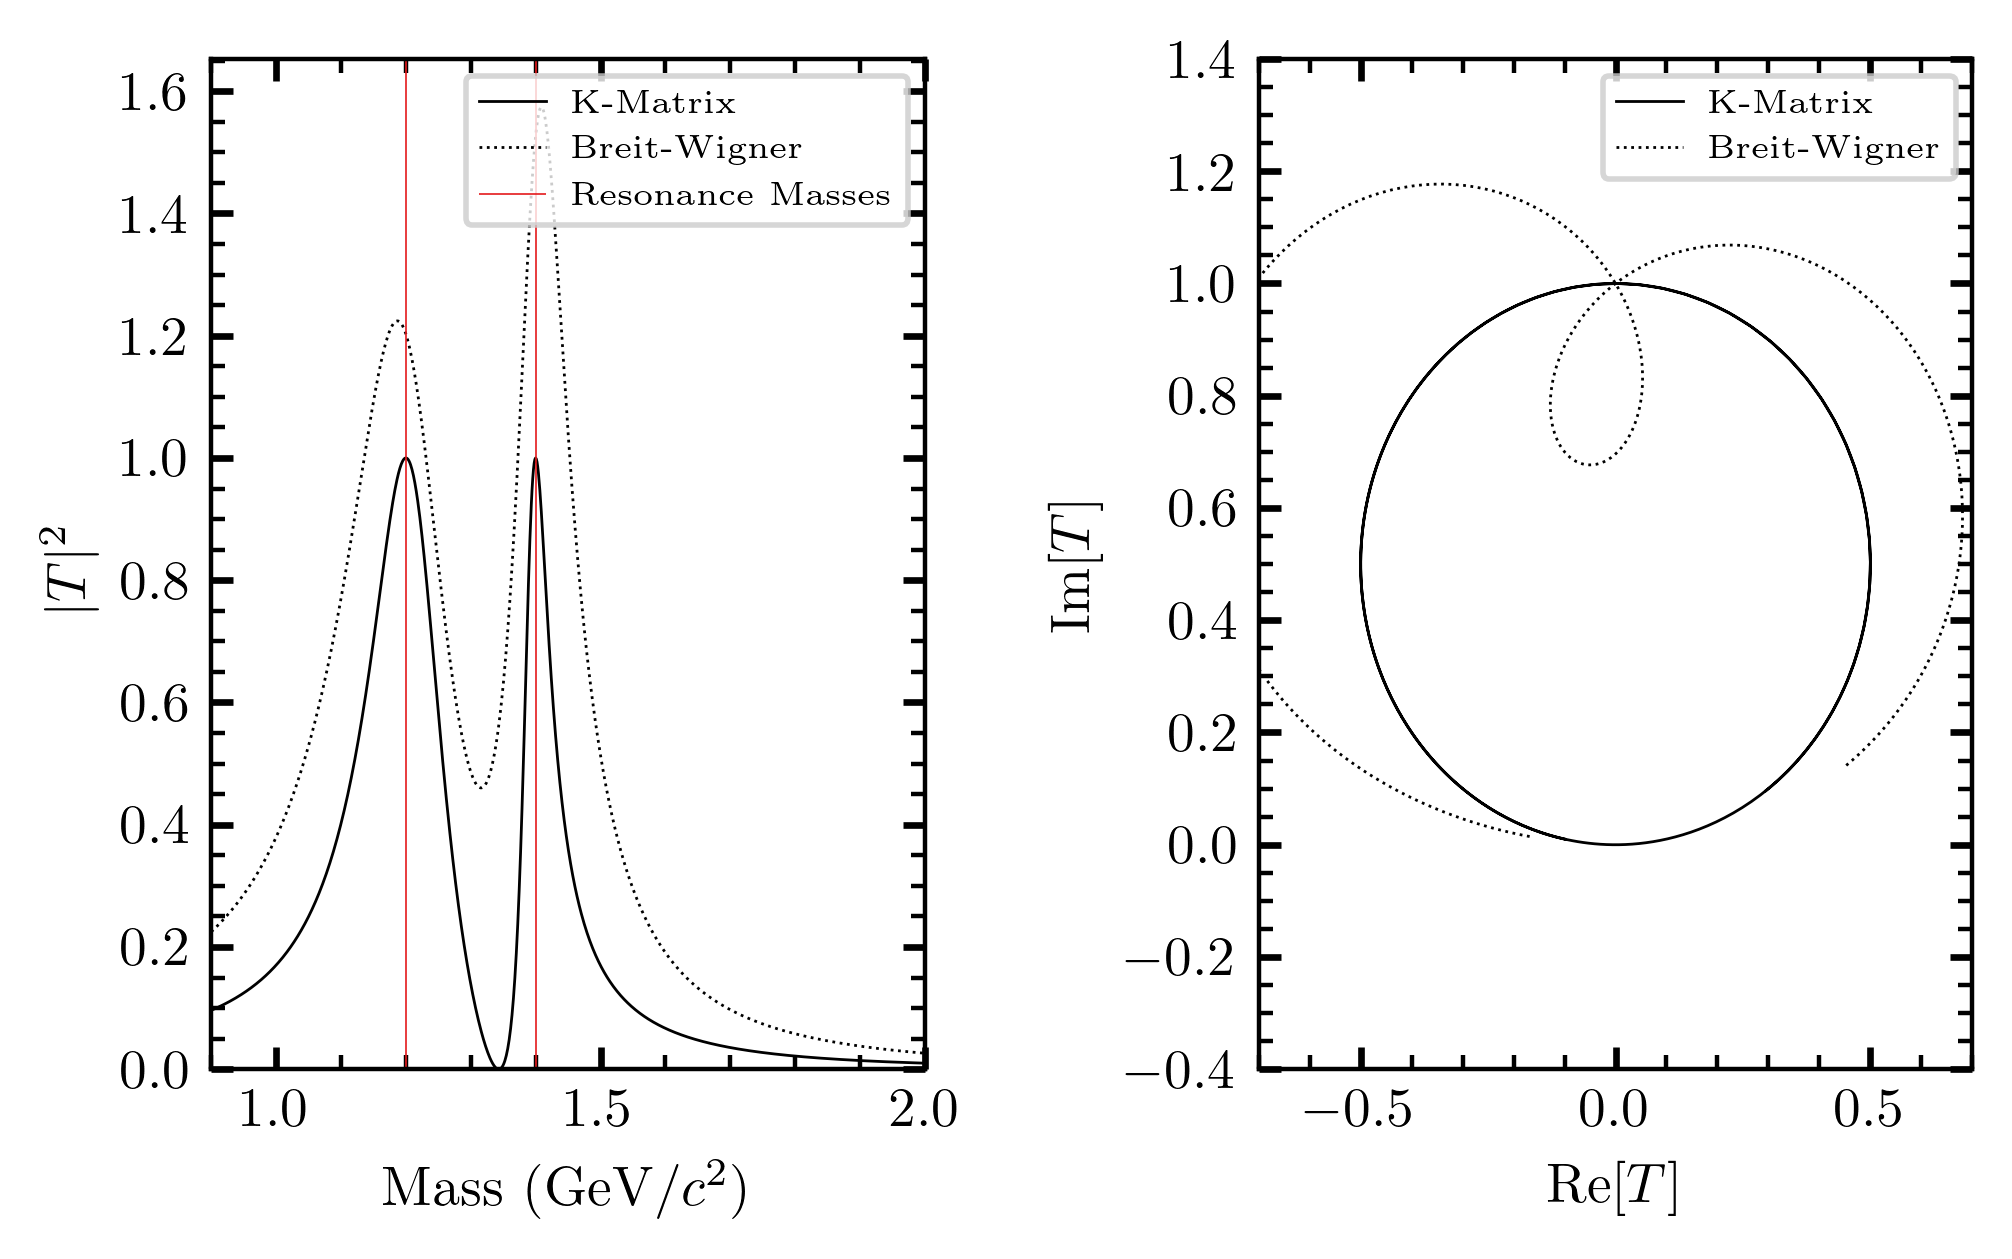
\includegraphics[width=0.8\textwidth]{figures/argand_diagram.png}
  \end{center}
  \caption{An Argand diagram depicting two fictitious resonances with masses of $\SI{1.2}{\giga\eV}/c^2$ and $\SI{1.4}{\giga\eV}/c^2$ and widths of $\SI{200}{\mega\eV}/c^2$ and $\SI{100}{\mega\eV}/c^2$ respectively using both the $K$-matrix formalism and interfering Breit-Wigners. The $T$-matrix formed from Breit-Wigners exceeds the unitary circle, implying that this construction breaks unitarity, while the $K$-matrix does not.}\label{fig:argand-diagram}
\end{figure}

\subsection{Resonances as Poles of the $K$-matrix}

Resonances can be parametrized either as constant elements in the $K$-matrix, which are usually interpreted as ``molecular'' resonances resulting from the exchange of force-carrying bosons, or from poles, which are thought of as the resonances describing decaying hadrons~\cite{au_meson_1987}. While we are more interested in the second case, we will include a linear combination of poles and constant terms in the parameterization, as follows:

\begin{equation}
  K_{ij}(m) = \sum_{\alpha} \frac{g_{\alpha i}(m) g_{\alpha j}(m)}{m_\alpha^2 - m^2} + c_{ij}
  \label{eq:k-matrix-parameterization}
\end{equation}

Here, $\alpha$ indexes the resonances, with $m_\alpha$ corresponding to the pole mass\footnote{This is not necessarily the same value as the centroid of a Breit-Wigner fit to the same data.} of the $\alpha$th resonance and $g_{\alpha i}$ corresponding to a term coupling the $\alpha$th resonance to the $i$th decay channel. $c_{ij}$ denotes any constant terms mentioned in the previously.

For a single resonance in a single channel, we can write the $T$-matrix as

\begin{align}
  T &= K(I-\imath K)^{-1} \\
    &= \frac{\frac{g^2(m)}{m_\alpha^2 - m^2}}{1 - \imath \left(\frac{g^2(m)}{m_\alpha^2 - m^2}\right)} \\
    &= \frac{g^2(m)}{m_\alpha^2 - m^2 - \imath g^2(m)}
\end{align}

which we see is identical to the Breit-Wigner form given in \Cref{eq:breit-wigner} with $g^2(m) = m_\alpha\Gamma_\alpha(m)$\footnote{Here, $\Gamma$ depends on $m$, which is true for a relativistic form of the Breit-Wigner amplitude.}.

Furthermore, we can now demonstrate the fundamental reason why we need to use the $K$-matrix in lieu of Breit-Wigners when describing multiple overlapping resonances. \Cref{fig:argand-diagram} shows that, even in a single channel, two interfering Breit-Wigners do not preserve unitarity, while the corresponding $K$-matrix does.

In the case where a resonance can decay into multiple channels, we say that $\Gamma_\alpha(m) = \sum_i \Gamma_{\alpha i}(m)$ is the total width and $\Gamma_{\alpha i}(m)$ are called the partial widths. In the relativistic form of the Breit-Wigner (and the Lorentz-invariant form of the resulting $S$-matrix), widths (and therefore partial widths) are given by

\begin{equation}
  \Gamma_{\alpha i} = \gamma^2_{\alpha i} \Gamma_{\alpha} B^\ell_{\alpha i}(m) \sqrt{\rho_i(m)}
  \label{eq:partial-width}
\end{equation}

where $\gamma^2_{\alpha i}$ is the fraction of the total width\footnote{However, $\gamma_{\alpha i}$ may itself be negative so long as it is purely real.}, $\Gamma_\alpha$, which is coupled to the channel $i$, and $\rho_i(m)$ is the phase space factor

\begin{equation}
  \rho_i(m) = \sqrt{\chi^+_i(m)\chi^-_i(m)}\quad\text{where}\quad\chi^{\pm}_i = 1 - \left(\frac{m_1 \pm m_2}{m}\right)^2
  \label{eq:rho}
\end{equation}

when the $i$th channel describes the decay $\alpha \to 1 + 2$ and $B^\ell_{\alpha i}(m)$ is the centrifugal barrier factor describing the suppression to the partial width when a resonance has angular momentum $\ell$. We typically parameterize this via form factors derived by Blatt and Weisskopf~\cite{blatt_theoretical_1979},

\begin{align}
  B^\ell_{\alpha i}(m) &= \frac{F_\ell(z_i(m))}{F_\ell(z_i(m_\alpha))} \\
  z_i(m) &\equiv \left(\frac{q_i(m)}{q_R}\right)^2 \\
  F_0(z) &= 1 \\
  F_1(z) &= \sqrt{\frac{2z}{z+1}} \\
  F_2(z) &= \sqrt{\frac{13z^2}{(z-3)^2 + 9z}} \\
  F_\ell(z) &= \sqrt{\frac{\abs{h_\ell^{(1)}(1)}^2}{z\abs{h_\ell^{(1)}(\sqrt{z})}^2}}
\end{align}

where $q_i(m) = m\rho_i(m)/2$ is the breakup momentum for the $i$th channel\footnote{i.e. the magnitude of the momentum either decay product will have in the rest frame of the decay}, $q_R$ is the impact parameter/interaction radius (we use $\SI{0.1973}{\giga\eV}$ in our calculations), and $h_\ell^{(1)}$ is a spherical Hankel function of the first kind (see Equation 2.4 of \cite{von_hippel_centrifugal-barrier_1972})

For clarity, we typically reparameterize these partial widths such that

\begin{equation}
  g_{\alpha i}(m) = g_{\alpha i}B^\ell_{\alpha i}(m)\sqrt{\rho_i(m)}
  \label{eq:coupling-expansion}
\end{equation}

so we can define the Lorentz-invariant $K$-matrix, $\hat{K}$, as

\begin{align}
  K_{ij}(m) &= \sqrt{\rho_i(m)}\left(\sum_{\alpha}B^\ell_{\alpha i}(m)\left[\frac{g_{\alpha i}g_{\alpha j}}{m_\alpha^2 - m^2} + \sum_n \bar{c}_{nij} m^{2n}\right]B^\ell_{\alpha j}\right)\sqrt{\rho_j(m)} \notag\\
  K_{ij}(m) &= \sqrt{\rho_i(m)} \hat{K}_{ij}(m) \sqrt{\rho_j(m)} \\
  \label{eq:invariant-k-matrix}
\end{align}

where we have absorbed some multiplicative factors into $c_{ij}$ to form the series expansion over powers of $m^2$ (since $\rho(m)$ and $B^\ell_{\alpha i}(m)$ only contain even powers of $m$) with coefficients $\bar{c}_{ij}$. Here, $\bar{K}$ replaces $K$ in \Cref{eq:t-matrix-from-k-matrix} as an intermediate step to defining a Lorentz-invariant formulation.

According to Chung\cite{chung_spin_1971}, the Lorentz-invariant form of the $T$-matrix, $\hat{T}$ can be written as

\begin{equation}
  T = \sqrt{\rho}\hat{T}\sqrt{\rho}
\end{equation}

where we define the notation

\begin{align}
  \rho_{ij}(m) &\equiv \rho_i(m)\delta_{ij}\\
  \sqrt{\rho_{ij}(m)} &\equiv \sqrt{\rho_i(m)}\delta_{ij}
\end{align}

In terms of \Cref{eq:t-matrix-from-k-matrix,eq:invariant-k-matrix,eq:k-t-inverse-relation}, we can write

\begin{equation}
  \hat{K}^{-1} = \hat{T}^{-1} + \imath \rho
\end{equation}

Following the previous derivation with these invariant forms, we find that

\begin{equation}
  \hat{T} = (I - \imath\hat{K}\rho)^{-1}\hat{K}
  \label{eq:t-matrix-from-k-matrix-invariant}
\end{equation}


\subsubsection{Production Amplitudes from a $K$-Matrix}

The $T$-matrix given in \Cref{eq:t-matrix-from-k-matrix-invariant} describes $s$-channel resonances (as in $a + b \to X \to c + d$). We can transform this into a production amplitude following Aitchison~\cite{aitchison_k-matrix_1972}:

\begin{equation}
  \hat{F} = (I - \imath\hat{K}\rho)^{-1}\hat{P}
  \label{eq:k-matrix-production-amplitude}
\end{equation}
where
\begin{equation}
  \hat{P}_i(\vec{\beta}; m) = \sum_\alpha \left(\frac{\beta_\alpha g_{\alpha i}}{m_\alpha^2 - m^2} + \sum_n c_{ni} m^{2n} \right)B_{\alpha i}^{\ell}(m)
  \label{eq:p-vector}
\end{equation}

Here, $\beta_\alpha$ describes the complex coupling from the initial state to the resonance $\alpha$. This can be thought of like a coupling coefficient in front of a single Breit-Wigner. The polynomial of coefficients are included for completeness, as any constant terms in $P$ preserve unitarity in the same way as constant terms in $K$, and the division of the factor of $\rho_i(m) \sim \rho_i(m^2)$ from \Cref{eq:coupling-expansion} and $B^\ell_{\alpha i}(m) \sim B^\ell_{\alpha i}(m^2)$ creates the given form.

\subsubsection{The Chew-Mandelstam Matrix}

For reasons which will become clear, we will define the diagonal matrix $C$, called the Chew-Mandelstam matrix, with the property

\begin{equation}
  \Im[C(m)] = -\rho(m)\quad\text{or}\quad C(m) = A(m) - \imath\rho(m)
\end{equation}
for some real function $A(m)$. It can be shown that we can replace $-\imath\rho$ in \Cref{eq:t-matrix-from-k-matrix-invariant} with such a matrix $C$ and still retain a valid $K$-matrix representation~\cite{wilson_resonances_2015},

\begin{equation}
  \hat{T} = (I + \hat{K}C)^{-1}\hat{K}
\end{equation}

and

\begin{equation}
  \hat{F} = (I + \hat{K}C)^{-1}\hat{P}
  \label{eq:k-matrix-production-amplitude-chew}
\end{equation}

The exact form of $A(m)$ is arbitrary, but we will be using

\begin{equation}
  C_{ii}(m) = C((m_1 + m_2)^2) + \frac{\rho_i(m)}{\pi}\ln\left[\frac{\chi^+_i(m) + \rho_i(m)}{\chi^+_i(m) - \rho_i(m)}\right] - \frac{\chi^+_i(m)}{\pi}\frac{m_2 - m_1}{m_1 + m_2}\ln\frac{m_2}{m_1}
  \label{eq:chew-mandelstam}
\end{equation}

where $m_1$ and $m_2$ are the masses of the final state of the $i$th decay channel, and we can choose $C((m_1 + m_2)^2) = 0$ for normalization. See \cite{oller_nd_1999}, \cite{basdevant_unitary_1977}, \cite{oller_chiral_2001}, and \cite{reid_generating_1984} for derivations and additional details of this expression. The motivation for this choice is that it behaves better below threshold than $\rho(m)$, as can be seen in \Cref{fig:chew-mandelstam}.

\begin{figure}
  \begin{center}
    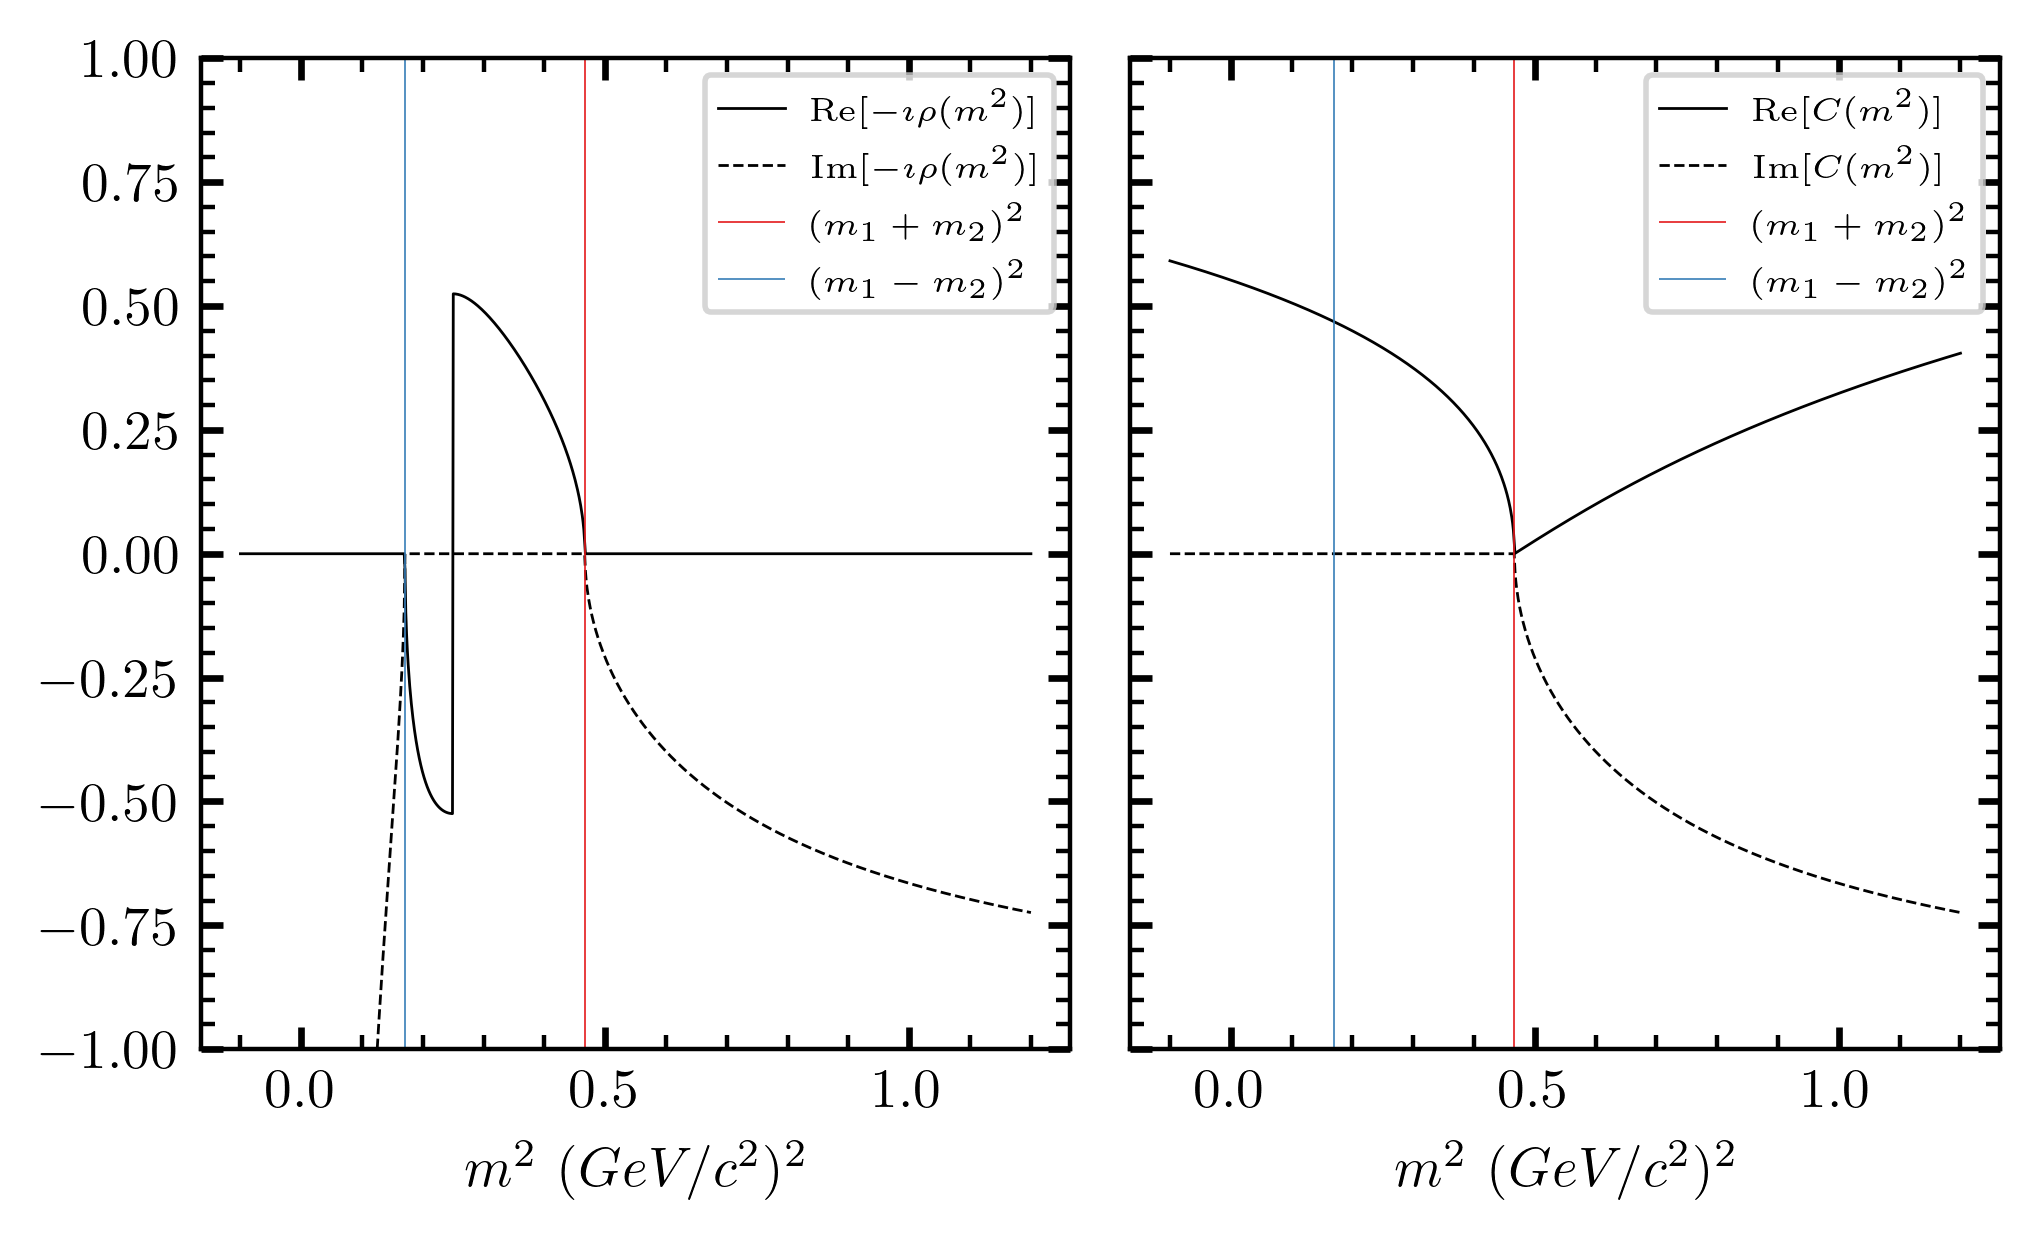
\includegraphics[width=0.8\textwidth]{figures/chew_mandelstam.png}
  \end{center}
  \caption{A comparison of the normal phase-space function, $\rho(m)$ (left) and the Chew-Mandelstam matrix, $C(m)$ (right) on the $\pi^0\eta$ channel. Both functions have the same imaginary part above the threshold $m = m_1 + m_2$, but phase-space function has a branch cut at $m^2 = \frac{(m_1^2 - m_2^2)^2}{m_1^2 + m_2^2}$ (the jump in the left plot between the red and blue lines) as well as a discontinuity at $m^2 = (m_1 - m_2)^2$ in both real and imaginary parts.}\label{fig:chew-mandelstam}
\end{figure}


The impetus of this complication is that this particular formulation of the Chew-Mandelstam matrix is used in \cite{albrecht_coupled_2020} and \cite{kopf_investigation_2021}. We do not have enough data to constrain the pole positions of every resonance in this channel (as we only have access to one of several channels used in those papers), so we will use the $K$-matrix coefficients ($g_{i\alpha}$ and $m_\alpha$) from their coupled-channel analysis of data from the Crystal Barrel and COMPASS experiments as fixed values in our analysis, fitting only the couplings ($\vec{\beta}$) to photoproduction. Additionally, using the results from these papers requires a Adler zero term in front of the $K$-matrix for the $f_0$ mesons of the form $\frac{(s - s_0)}{s_\text{norm}}$, where they use $s_0 = m^2_{\pi_0}/2$ and $s_\text{norm} = 1$.

We can then combine \Cref{eq:k-matrix-production-amplitude-chew} with \Cref{eq:generalized-polarized-intensity}, choosing $T^{J(\epsilon)}_{M;\eta}(\vec{\beta}; m) = \hat{F}(\vec{\beta}; m)$, to form a mass-dependent model of polarized photoproduction for the $K_S^0K_S^0$ channel which will be further discussed in \Cref{sec:mass-dependent-fits}.

\section{Waveset Selection}

\chapter{Results and Systematic Studies}
\section{Fitting Methods}\label{sec:fitting-methods}

To fit the aforementioned models to the data, we employ an algorithm which maximizes the likelihood function,
\begin{equation}
  \mathcal{L}(\vec{\beta}) = e^{-\mathcal{N}} \frac{\mathcal{N}^N}{N!} \prod_{i=1}^{N} \mathcal{P}_i(\vec{\beta}),
  \label{eq:likelihood}
\end{equation}
where $N$ is the number of events in the data, $\mathcal{N}$ is the number of events predicted by the model, and $\mathcal{P}_i(\vec{\beta})$ is the normalized probability distribution function evaluated on the $i$th event at position $\vec{\beta}$ in parameter space. The term in front of the product is a Poisson distribution which describes the ``extended'' maximum likelihood method. We relate these probability distributions to our modeled intensity function in \Cref{eq:generalized-polarized-intensity} via the normalization,
\begin{equation}
  \mathcal{I}(\vec{\beta}; m_i, s_i, \Omega_i, P_{\gamma, i}, \Phi_i) \equiv \mathcal{I}_i(\vec{\beta}) = \mathcal{N}\mathcal{P}_i(\vec{\beta}).
\end{equation}

By absorbing the factor of $\mathcal{N}^N$ into the product, we find

\begin{equation}
  \mathcal{L}(\vec{\beta}) = \frac{e^{-\mathcal{N}}}{N!} \prod_{i=1}^{N} \mathcal{I}_i(\vec{\beta}).
\end{equation}

We want to maximize this function, but the product makes this computationally difficult and unstable, since it can grow very large (if $\mathcal{I} > 1$) or very small (if $\mathcal{I} < 1$) to a point where its value exceeds floating-point precision. The standard solution is to instead minimize the negative logarithm of the likelihood instead,

\begin{equation}
  -2 \ln \mathcal{L}(\vec{\beta}) = -2 \left(\sum_{i=1}^{N} \left[\ln \mathcal{I}_i(\vec{\beta})\right] - \mathcal{N} - \ln N! \right),
\end{equation}
where the factor of two scales the log-likelihood to correspond to a $\chi^2$ distribution as $N \to \infty$ by Wilks' theorem, allowing us to obtain an accurate covariance matrix from the fit for uncertainty estimation.

In an ideal world, we could stop here, ignoring the last two terms as they are constant in $\beta$ and therefore do not contribute to the gradient of the negative log-likelihood. However, we must also consider the efficiency of the detector itself, which we will define as $\eta(m_i, s_i, \Omega_i, P_{\gamma,i}, \Phi_i) \equiv \eta_i$. In principle, we do not know the analytical form of this function, but we will later see that we can approximate it using Monte Carlo simulated data.

With this efficiency function in mind, we find that $\mathcal{N}$, the normalization factor which describes the number of events predicted by the model, becomes

\begin{equation}
  \mathcal{N} = \int \dd{\vec{x}} \mathcal{I}(\vec{\beta}; \vec{x})\eta(\vec{x}),
\end{equation}
where $\vec{x} = (m, s, \Omega, P_{\gamma}, \Phi)$. This means we can write the normalized probability distribution functions as

\begin{equation}
  \mathcal{P}_i(\vec{\beta}) = \frac{1}{\mathcal{N}} \mathcal{I}_i(\vec{\beta})\eta_i.
\end{equation}

This changes the negative log-likelihood to

\begin{align}
  - 2 \ln \mathcal{L}(\vec{\beta}) &= -2 \left( \sum_{i=1}^N \left[\ln \mathcal{I}_i(\vec{\beta})\right] - \int \dd{\vec{x}} \mathcal{I}(\vec{\beta; \vec{x}})\eta(\vec{x}) - \ln N! + \sum_{i=1}^N \left[\ln\eta_i\right]\right) \\
                                   &= -2 \left( \sum_{i=1}^N \left[\ln \mathcal{I}_i(\vec{\beta})\right] - \int \dd{\vec{x}} \mathcal{I}(\vec{\beta; \vec{x}})\eta(\vec{x})\right) + C.
\end{align}

Next, we need a way of dealing with the integral term, particularly with the $\eta(\vec{x})$ function for which we do not have access to the analytical form. To approximate this integral, we use both the fundamental theorem of calculus and the mean value theorem for derivatives, which together relate the integral of a function to its average value on the domain of integration,

\begin{equation}
  \int_{\mathbb{D}} f(\vec{x})\dd{\vec{x}} = \mathbb{A} \ev{f(\vec{x})},
  \label{eq:mean-value-theorem}
\end{equation}
where $\mathbb{A}$ is the area of the integration domain $\mathbb{D}$ and $\ev{f(\vec{x})}$ denotes the average value of $f(\vec{x})$ on that domain. If we generate phase-space Monte Carlo for the $K_S^0K_S^0$ channel, we can model $\eta(\vec{x})$ as an indicator function corresponding to whether or not an event is detected by a simulation of the detector, passes through the reconstruction process described in \Cref{sub:particle-identification-and-the-gluex-kinematic-fit}, and passes through our finer data selection from \Cref{sub:fiducial-cuts}. We can then write the average as a sum over the ``accepted'' Monte Carlo events,

\begin{equation}
  \int \dd{\vec{x}} \mathcal{I}(\vec{\beta}; \vec{x})\eta(\vec{x}) = \frac{1}{\mathbb{A} N_g} \sum_{j=1}^{N_a} \left[\mathcal{I}_j(\vec{\beta})\right],
\end{equation}
where $\mathcal{I}_j(\vec{\beta})$ is evaluated on the $j$th accepted Monte Carlo event\footnote{This is not to be confused with $\mathcal{I}_i(\vec{\beta})$, which we will use to refer to the function evaluated over data. These terms will always stay in separate sums for clarity.}, and $N_a$ and $N_g$ are the number of accepted and generated events, respectively. We still need to deal with the factor of $\mathbb{A}$. We could absorb this into our intensity function by scaling the intensity by $\mathbb{A}^{N_a}$, which would eliminate it from this term. In the data term, we would then have

\begin{equation}
  \sum_{i=1}^N \left[\mathbb{A}^{N_a}\mathcal{I}_i(\vec{\beta})\right] = \sum_{i=1}^N \left[\mathcal{I}_i(\vec{\beta})\right] + NN_a\ln\mathbb{A},
\end{equation}
where the new additive term is constant in $\vec{\beta}$ and can again be ignored in the minimization. At this stage, we need to minimize

\begin{equation}
  -2\ln\mathcal{L}(\vec{\beta}) = -2\left(\sum_{i=1}^N\left[\ln\mathcal{I}_i(\vec{\beta})\right] - \frac{1}{N_g} \sum_{i=j}^{N_a}\left[\mathcal{I}_j(\vec{\beta})\right]\right).
\end{equation}

We can incorporate event weights (from accidental subtraction or sPlot, for example) into these sums as

\begin{equation}
  -2\ln\mathcal{L}(\vec{\beta}) = -2\left(\sum_{i=1}^N\left[w_i\ln\mathcal{I}_i(\vec{\beta})\right] - \frac{1}{N_g} \sum_{i=j}^{N_a}\left[w_j\mathcal{I}_j(\vec{\beta})\right]\right)
\end{equation}

An additional scaling of the intensity with $\mathcal{I}(\vec{\beta}) \to \varepsilon^{-N_{\alpha}}\mathcal{I}(\vec{\beta})$ with $N_g = \varepsilon N_a$ can be made to eliminate $N_g$ from this expression, which adds a constant factor of $-NN_a\ln\varepsilon$ to the negative log-likelihood. This choice is optional, but it can be helpful from a computational/organizational standpoint when it comes to projecting the fitted model back onto each Monte Carlo dataset and is chosen in this analysis to give us

\begin{equation}
  -2\ln\mathcal{L}(\vec{\beta}) = -2\left(\sum_{i=1}^N\left[w_i\ln\mathcal{I}_i(\vec{\beta})\right] - \frac{1}{N_a} \sum_{i=j}^{N_a}\left[w_j\mathcal{I}_j(\vec{\beta})\right]\right).
\end{equation}

We can now choose a minimization algorithm to fit our data to various models which will be described in detail in \Cref{sec:mass-independent-fits,sec:mass-dependent-fits}. For this analysis, fits were performed with \texttt{laddu}, an amplitude analysis engine I wrote, which uses the L-BFGS-B minimization algorithm, a memory-efficient variant of the Broyden-Fletcher-Goldfarb-Shanno algorithm which allows for box constraints on the parameter space~\cite{Byrd1995}.

To obtain plots of the fitted model, we can weight each event in either the accepted or generated Monte Carlo (for results without and with efficiency correction, respectively) as,

\begin{equation}
  \hat{w}_j = \frac{w_j \mathcal{I}_j(\vec{\beta}^*)}{N_\text{MC}},
\end{equation}
where $\vec{\beta}^*$ is the value of the fit parameters which maximizes the likelihood and $N_\text{MC}$ is $N_a$ or $N_g$ depending on which set of Monte Carlo we are using. We can additionally isolate individual waves by manually setting the coefficients of other waves to zero before evaluating the intensity.

\section{Mass-Independent Fits}\label{sec:mass-independent-fits}

\subsection{Waveset Selection}

Assuming only spin-$0$ and spin-$2$ waves, (notated $S$- and $D$-waves respectively) are present in this system, the generalized intensity function in \Cref{eq:generalized-polarized-intensity} allows for two $S$-waves (one of each reflectivity) and ten $D$-waves (five for each reflectivity, with $M=+2$, $+1$, $0$, $-1$, or $-2$). Choosing which waves to include is not a trivial matter. For example, if we tried including all possible waves, Uns\"old's theorem tells us that an unweighted combination of all $D$-waves is constant in angle~\cite{Unsld1927}, so we should expect some degree of leakage from between the $S$- and $D$-waves. The limited dataset will only make this problem worse, as the data may lack the statistical power to distinguish between the many kinds of $D$-waves. Furthermore, a larger waveset includes more free parameters and is more vulnerable to overfitting. It is therefore our prerogative to model the data with the smallest possible waveset which we believe describes the data.

For the remainder of this thesis, we will refer to each wave via the notation $L_m^{(\epsilon)}$ where $L$ is the letter corresponding to the total angular momentum ($S$ or $D$), $m$ is the eigenvalue of angular momentum projection onto the $z$-axis, and $\epsilon$ is the sign of the reflectivity. With this notation, $S_0^{(-)}$ represents the spin-$0$ wave with negative reflectivity and $D_{-2}^{(+)}$ is the spin-$2$ wave with positive reflectivity and $m=-2$ spin projection.

We begin by isolating the positive reflectivity waves. If we look at the potential resonances in \Cref{fig:mass-with-pdg}, we can expect to see $S$-wave components across the entire dataset, so we will always include an $S$-wave. As for which $D$-wave(s) to include, we can begin by fitting each of $D_{+2}^{(+)}$, $D_{+1}^{(+)}$, and $D_{0}^{(+)}$, since the negative-$m$ projections only differ by the sign of $\varphi$\footnote{If we were to include more than one $D$-wave, then the sign of $m$ would matter.}.

\begin{figure}
  \begin{center}
    \includegraphics[width=0.8\textwidth]{ext/analysis/plots/meson_pdg_data_pz_masscut_chisqdof_3.0_mesons_free_2.png}
  \end{center}
  \caption{The invariant mass of $K_S^0K_S^0$ plotted alongside expected resonances from the PDG~\cite{Zyla2020}. Each rectangle represents a resonance, and the position and width of the rectangle corresponds to the mass and width of the resonance in the PDG. Unfilled rectangles represent particles which have not been firmly established by experiment. There is no meaning to the vertical positioning of the rectangles other than the grouping of spin-$0$ and spin-$2$ resonances on either side of the dotted line.}\label{fig:mass-with-pdg}
\end{figure}

To get an idea of what we might expect to see in these fits, we can examine the distribution of $\cos\theta_\text{HX}$ with respect to the invariant mass in \Cref{fig:costheta-vs-mass}. If we think of binning in mass as akin to slicing this figure into vertical strips, then we can compare each bin to the expected shape of the waves in \Cref{fig:spherical-harmonics}. In this way, we might expect the region in $\qtyrange{1.2}{1.6}{\giga\electronvolt}$ to predominantly correspond to the $m=\pm 2$ projection (along with an $S$-wave), since the distribution peaks at the center and falls off at the extreme forward and backward angles. A $D_0$ wave would also peak in the center, but we would expect it to grow rapidly in the forward and backward directions. Similarly, a $D_1$ wave would decay in the forward and backward directions, but would also show a dip in the center.

\begin{figure}
  \begin{center}
    \includegraphics[width=0.8\textwidth]{ext/analysis/plots/costheta_hx_v_meson_mass_data_pz_masscut_chisqdof_3.0_mesons_free_2.png}
  \end{center}
  \caption{A plot of the distribution of $\cos\theta_\text{HX}$ with respect to the invariant mass after all analysis selections and weightings have been applied. This figure is a repeat of \Cref{fig:costheta-hx-v-meson-mass-data-pz-masscut-chisqdof-3.0-mesons-free-2} included here for convenience.}\label{fig:costheta-vs-mass}
\end{figure}

\begin{figure}
  \begin{center}
    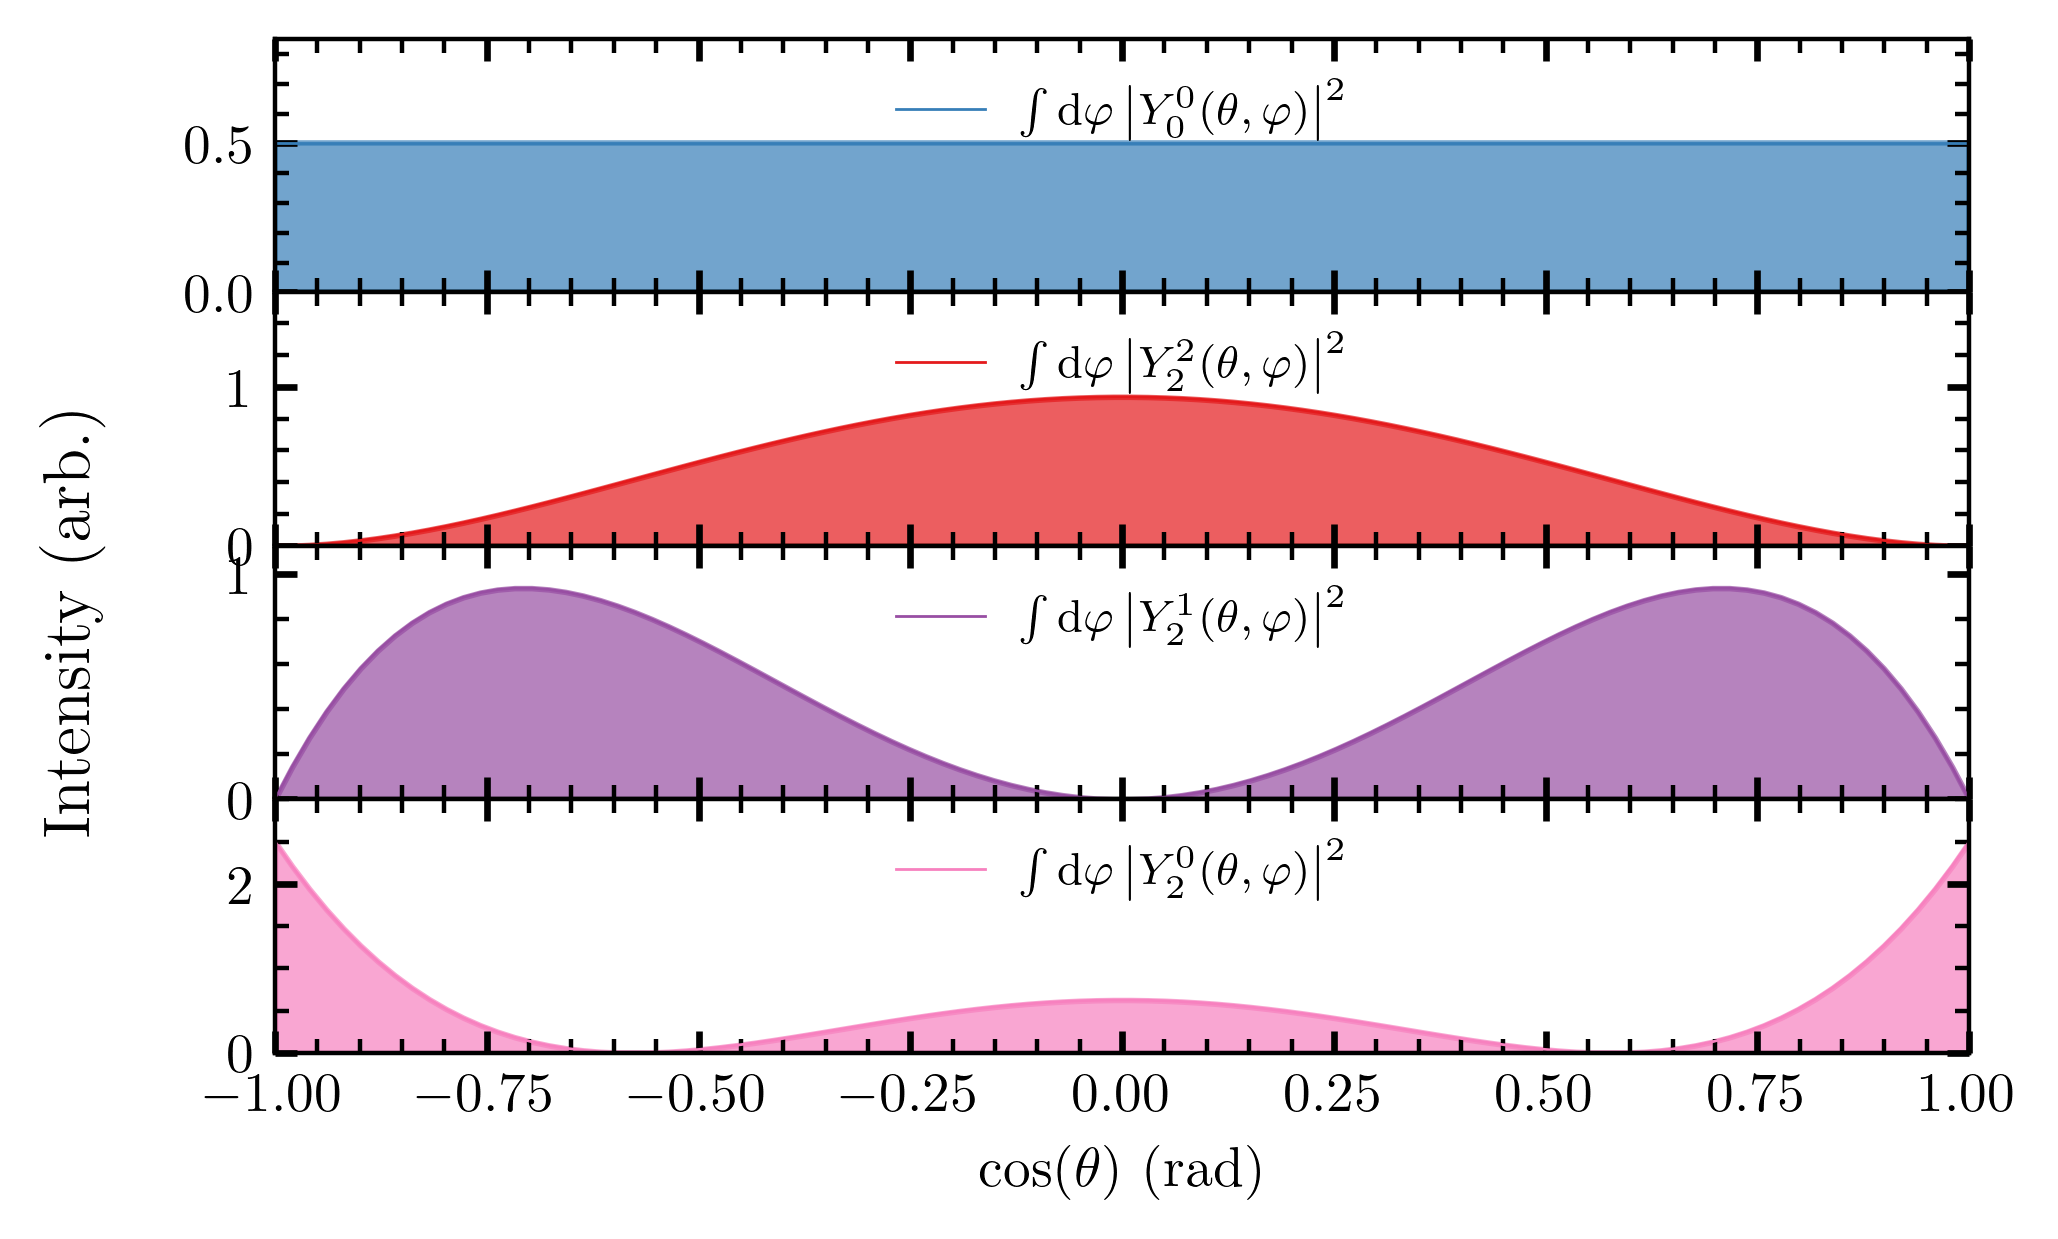
\includegraphics[width=0.8\textwidth]{ext/analysis/plots/spherical_harmonics.png}
  \end{center}
  \caption{The expected normalized projections of several spherical harmonics which may be present in the data, integrated over $\varphi$, the polar angle.}\label{fig:spherical-harmonics}
\end{figure}

Examining the angular distribution is a good first step, but it is more prudent to perform fits with each wave to see how well they represent the data. The fitting procedure begins with dividing the data into bins of invariant $K_S^0K_S^0$ mass. In each bin, we fit \Cref{eq:generalized-polarized-intensity} via the method described in \Cref{sec:fitting-methods}. We let each $\hat{T}_{M;\eta}^{J(\epsilon)}$ be a free complex parameter in each bin\footnote{We ignore the sum over the nucleon spin-flip index, $\eta$, since it is not measurable by this experiment.}. The $S$-wave amplitude is just given by a real scalar parameter, since the total form of the intensity is invariant up to a total phase in each coherent sum\footnote{Similarly, when negative reflectivity waves are included, the $S_0^{(-)}$ wave will also be purely real.}. Each bin in mass is fit independently, and the results can be seen in \Cref{fig:binned-fit-chisqdof-3.0-Sp-D0p,fig:binned-fit-chisqdof-3.0-Sp-D1p,fig:binned-fit-chisqdof-3.0-Sp-D2p}. It appears our visual examination of \Cref{fig:costheta-vs-mass} was indeed descriptive, since only the $D_2^{(+)}$ wave has a significant projection onto the data.

Additionally, the binned fit for this wave exhibits two clear peaks, one at around $\SI{1.3}{\giga\electronvolt}$ and one around $\SI{1.5}{\giga\electronvolt}$. We expect these to correspond to the well-established $f_2(1270)$, $a_2(1320)$, and $f_2'(1525)$ resonances (see \Cref{tab:pdg-resonances}). 


\begin{table}
  \begin{center}
    \begin{tabular}{ccc}\toprule
      Resonance & Mass ($\si{\mega\electronvolt}/c^2$) & Width ($\si{\mega\electronvolt}/c^2$)\\\midrule
      $f_0(500)^{\ast}$ & $400$\textendash$800$ & $100$\textendash$800$ \\
      $f_0(980)$ & $990\pm 20$ & $10$\textendash$100$ \\
      $a_0(980)$ & $980\pm 20$ & $50$\textendash$100$ \\
      $f_2(1270)$ & $1275.4 \pm 0.8$ & $186.6^{+2.8}_{-2.2}$ \\
      $a_2(1320)$ & $1318.2 \pm 0.6$ & $109.8\pm 2.4$ \\
      $f_0(1370)$ & $1200$\textendash$1500$ & $200$\textendash$500$ \\
      $f_2(1430)^{\ast\dagger}$ & $\approx 1430$ & $\approx 13$\textendash$43$ \\
      $a_0(1450)$ & $1439\pm 34$ & $258\pm 14$ \\
      $f_0(1500)$ & $1522\pm 25$ & $108\pm 33$ \\
      $f_2'(1525)$ & $1517.3\pm 2.4$ & $72^{+7}_{-6}$ \\
      $f_2(1565)^{\ast}$ & $1571\pm 13$ & $132\pm 23$ \\
      $f_2(1640)^{\ast\dagger}$ & $1639\pm 6$ & $100^{+60}_{-40}$ \\
      $a_2(1700)$ & $1706\pm 14$ & $380^{+60}_{-50}$ \\
      $a_0(1710)^{\ast\dagger}$ & $1713\pm 19$ & $107\pm 15$ \\
      $f_0(1710)$ & $1733^{+8}_{-7}$ & $150^{+12}_{-10}$ \\
      $f_0(1770)^{\ast\dagger}$ & $1784^{+16}_{-14}$ & $161\pm 21$ \\
      $f_2(1810)^{\dagger}$ & $1815\pm 12$ & $197\pm 22$ \\
      $f_2(1910)^{\ast\dagger}$ & $1941\pm 182$ & $120\pm 40$ \\
      $a_0(1950)^{\ast\dagger}$ & $1931\pm 26$ & $270\pm 40$ \\
      $f_2(1950)$ & $1936\pm 12$ & $464\pm 24$ \\
      $f_2(2010)^{\ast}$ & $2010^{+60}_{-80}$ & $200\pm 60$ \\
      $f_0(2020)^{\ast}$ & $1982^{+54.1}_{-3.0}$ & $440\pm 50$ \\
      $f_0(2100)^{\ast\dagger}$ & $2095^{+17}_{-19}$ & $287^{+32}_{-24}$ \\
      $f_2(2150)^{\ast\dagger}$ & $2157\pm 12$ & $152\pm 30$ \\
      $f_0(2200)^{\ast\dagger}$ & $2187\pm 14$ & $210\pm 40$ \\\bottomrule
    \end{tabular}
    \caption{Resonances along with their approximate masses and widths from the PDG~\cite{Zyla2020} with quantum numbers compatible with the $K_S^0K_S^0$ channel. Resonances marked with an asterisk ($\ast$) are not included in the $K$-matrix model for the mass-dependent fits. Resonances marked with a dagger ($\dagger$) are not well-established according to the PDG.}\label{tab:pdg-resonances}
  \end{center}
\end{table}


\begin{figure}
  \begin{center}
    \includegraphics[width=0.8\textwidth]{ext/analysis/plots/binned_fit_pz_masscut_chisqdof_3.0_mesons_free_2_487_50_boot_30_CI-BC.png}
  \end{center}
  \caption{Binned fit of $S_{0}^{(+)}$ and $D_{0}^{(+)}$ waves. Bars on each fit point correspond to $68\%$ bias-corrected confidence intervals over $ 30 $ bootstrap iterations.}\label{fig:binned-fit-chisqdof-3.0-Sp-D0p}
\end{figure}
\begin{figure}
  \begin{center}
    \includegraphics[width=0.8\textwidth]{ext/analysis/plots/binned_fit_pz_masscut_chisqdof_3.0_mesons_free_2_489_50_boot_30_CI-BC.png}
  \end{center}
  \caption{Binned fit of $S_{0}^{(+)}$ and $D_{+1}^{(+)}$ waves. Bars on each fit point correspond to $68\%$ bias-corrected confidence intervals over $ 30 $ bootstrap iterations.}\label{fig:binned-fit-chisqdof-3.0-Sp-D1p}
\end{figure}
\begin{figure}
  \begin{center}
    \includegraphics[width=0.8\textwidth]{ext/analysis/plots/binned_fit_pz_masscut_chisqdof_3.0_mesons_free_2_491_50_boot_30_CI-BC.png}
  \end{center}
  \caption{Binned fit of $S_{0}^{(+)}$ and $D_{+2}^{(+)}$ waves. Bars on each fit point correspond to $68\%$ bias-corrected confidence intervals over $ 30 $ bootstrap iterations.}\label{fig:binned-fit-chisqdof-3.0-Sp-D2p}
\end{figure}

We can also sum the negative log-likelihoods from each bin in each fit to get a total likelihood for each fit. Since each fit has the same number of free parameters, we can directly compare the negative log-likelihoods, which are $-448,423.33$, $-447,961.96$, and $-449,203.72$ (smaller is better) for the fits involving $D_0^{(+)}$, $D_1^{(+)}$, and $D_2^{(+)}$ waves respectively. We can conclude that the $D_2^{(+)}$ wave model is the most likely to describe the data, since it has the lowest negative log-likelihood.

While we could imagine that interference effects between waves could cause the non-$D_2$ waves to have a non-negligible projection onto the data, we must focus on the minimal set of waves required to fit the data. The next wave we will add to this model will be a negative-reflectivity $S$-wave. In the model, waves only interfere with waves of the same reflectivity, so we should expect the $D$-wave to be largely unaffected by this additional wave. However, since the existing $S_0^{(+)}$ wave will be reduced non-trivially in each bin, it is possible that the $D_2^{(+)}$ wave projection may change slightly in regions where the $S_0^{(-)}$ component is large. We can see the result of this fit in \Cref{fig:binned-fit-chisqdof-3.0-Spn-D2p}. The notable difference between this fit and the previous fit without the $S_0^{(-)}$ wave is that the $S_0^{(+)}$ wave no longer has the large bump around $\SI{1.5}{\giga\electronvolt}$ which was likely due to a combination of the $a_0(1450)$ and $f_0(1500)$. Instead, we still see a slight enhancement in the positive-reflectivity $S$-wave, but there is a much more noticeable peak in the negative-reflectivity $S$-wave right at $\SI{1.5}{\giga\electronvolt}$. Referencing \Cref{tab:pdg-resonances}, there is only one narrow spin-$0$ resonance around this mass, viz. the $f_0(1500)$. Since positive/negative reflectivity corresponds to natural/unnatural parity exchange in this $t$-channel interaction, the fit may suggest that $f_0(1500)$ production is mostly produced by some unnatural parity exchange process, or at least some percentage of the resonant production follows a different production process.

\begin{figure}
  \begin{center}
    \includegraphics[width=0.8\textwidth]{ext/analysis/plots/binned_fit_pz_masscut_chisqdof_3.0_mesons_free_2_29099_50_boot_30_CI-BC.png}
  \end{center}
  \caption{Binned fit of $S_{0}^{(+)}$, $S_{0}^{(-)}$, and $D_{+2}^{(+)}$ waves. Bars on each fit point correspond to $68\%$ bias-corrected confidence intervals over $ 30 $ bootstrap iterations.}\label{fig:binned-fit-chisqdof-3.0-Spn-D2p}
\end{figure}

Since we have split the $S$-wave into reflectivity components, the next obvious step would be to also split the $D$-wave. We can see the result in \Cref{fig:binned-fit-chisqdof-3.0-Spn-D2pn}. The results are no longer as unambiguous, as there is a large amount of bin-to-bin fluctuation in the $D$-wave projections, but there is still some indication of two spin-$2$ peaks in the positive reflectivity component, and the peak around $\SI{1.5}{\giga\electronvolt}$ does not appear to have as strong of a negative reflectivity component.

\begin{figure}
  \begin{center}
    \includegraphics[width=0.8\textwidth]{ext/analysis/plots/binned_fit_pz_masscut_chisqdof_3.0_mesons_free_2_1862378_50_boot_30_CI-BC.png}
  \end{center}
  \caption{Binned fit of $S_{0}^{(+)}$, $S_{0}^{(-)}$, $D_{+2}^{(+)}$, and $D_{+2}^{(-)}$ waves. Bars on each fit point correspond to $68\%$ bias-corrected confidence intervals over $ 30 $ bootstrap iterations.}\label{fig:binned-fit-chisqdof-3.0-Spn-D2pn}
\end{figure}

\subsection{Comparison to CLAS}\label{sub:comparison-to-clas}
As mentioned in \Cref{sec:past-analyses}, the most recent analysis of this channel and the only prior photoproduction analysis was performed by the CLAS collaboration~\cite{Chandavar2018}. Their results, presented in Table II of their paper, list the fraction of $S$-wave in a ``$S+B$'' region and a sideband region over multiple bins in invariant mass of $K_S^0K_S^0$. The $S+B$ region refers to a $3\sigma$ selection around a peak in the two-dimensional plot of the invariant mass of $\pi_1^+\pi_1^-$ and that of $\pi_2^+\pi_2^-$. The pion pairs are assigned randomly to avoid a combinatorial bias, and the sidebands consist of nine directly adjacent squares surrounding the signal peak in that plot, weighted proportionately. They then generated a pure $S$-wave and pure $D$-wave Monte Carlo sample and fit each to even polynomials in $\cos\theta$ in the Gottfried-Jackson frame. The fitted shapes where then used in a mixture model (without interference) to determine the ratio of $S$-wave to $D$-wave in each $K_S^0K_S^0$ invariant mass bin. While we do not have access to their dataset, we can project these ratios (and their uncertainties\footnote{If the $S$-wave fraction in a bin is $f\pm\sigma_f$ and the number of events in that bin of our dataset is $n\pm\sigma_n$, we calculate the size of the $S$-wave contribution as $(n\times f) \pm \sqrt{(f\sigma_n)^2 + (n\sigma_f)^2}$}) onto our dataset and compare them to the results of our analysis. The comparison for the $S+B$ region and the sideband region can be seen in \Cref{fig:clas-comparison-SB} and \Cref{fig:clas-comparison-sideband} respectively.

\begin{figure}
  \begin{center}
    \includegraphics[width=0.8\textwidth]{ext/analysis/plots/CLAS_peak_binned_fit_pz_masscut_chisqdof_3.0_mesons_free_2_491_20_boot_30_CI-BC.png}
  \end{center}
  \caption{Binned fit of $S_0^{(+)}$ and $D_2^{(+)}$ waves from this analysis alongside projections from the CLAS analysis~\cite{Chandavar2018} over their $S+B$ region. Uncertainties are from $68\%$ bias-corrected confidence intervals and from reported error propagation respectively.}\label{fig:clas-comparison-SB}
\end{figure}

\begin{figure}
  \begin{center}
    \includegraphics[width=0.8\textwidth]{ext/analysis/plots/CLAS_sideband_binned_fit_pz_masscut_chisqdof_3.0_mesons_free_2_491_20_boot_30_CI-BC.png}
  \end{center}
  \caption{Binned fit of $S_0^{(+)}$ and $D_2^{(+)}$ waves from this analysis alongside projections from the CLAS analysis~\cite{Chandavar2018} over their sideband region. Uncertainties are from $68\%$ bias-corrected confidence intervals and from reported error propagation respectively.}\label{fig:clas-comparison-sideband}
\end{figure}

The interpretation of these results is not straightforward, since the CLAS analysis does not report the estimated size of the background in their $S+B$ region, so any interpretation of the sideband is problematic. However, we can say with confidence that their results are not consistent with ours across any region in $K_S^0K_S^0$ invariant mass aside from some bins in which we both find almost zero contribution from any $D$-wave. The lack of signal from any of the $f_2(1270)$, $a_2(1320)$, $f_2'(1525)$, or $f_2(1565)$ resonances is likely due to the limited acceptance of the CLAS detector, which makes it difficult to distinguish $S$-waves from $D$-waves.


\section{Mass-Dependent Fits}\label{sec:mass-dependent-fits}

We now turn our attention to the $K$-matrix formalism discussed in \Cref{sec:k-matrix}. We could restrict the $K$-matrix to a single channel and fit both the production couplings ($\beta_\alpha$) and decay couplings ($g_{i\alpha}$) along with the mass poles ($m_\alpha$), and this would ostensibly result in the same number of free parameters as would Breit-Wigner peaks for each resonance. However, the key point of the $K$-matrix is that it also describes the effect on resonances when a threshold energy is crossed and a channel is opened up, and this cannot be similarly captured with a single-channel approach. In the case of $K_S^0K_S^0$, the threshold production of the $f_0(980)$ and $a_0(980)$ is problematic for several reasons. First, both of these resonances have mass poles just smaller than the threshold for producing two $K_S^0$s, so the lineshape may be dependent on the coupling to other channels. Second, these particles differ only in isospin, which is not observable in the $K_S^0K_S^0$ channel. This makes it very difficult to control for the possible interference effects between the two resonances. Finally, the $\eta'\pi$ channel opens around $\SI{1.093}{\giga\electronvolt}$, and there is evidence that the $a_0(980)$ has a nonzero component in this channel~\cite{Ablikim2017,Chen2020}, and this may also alter the shape of the intensity from these resonances. We can attempt to circumvent the first two issues by using a fixed $K$-matrix. In principle, this is like fixing the masses and widths of a set of Breit-Wigner peaks to known values from literature. However, in practice, it allows us to incorporate some information about the effect of other channels on the intensity. We will use the results of \cite{Albrecht2020} and \cite{Kopf2021} as the basis for the $K$-matrix. This does not help us with the third problem, since the $\eta'\pi$ channel is not included in their fit for the $a_0$ $K$-matrix, but we will assume that their fit accurately covers the most prominent resonances in our region of interest. Using their published values for the decay couplings, mass peaks, and non-resonant background corrections ($\tilde{c}_{nij}$), we construct the $K$-matrix for the $f_0$, $a_0$, $f_2$, and $a_2$ channels accordingly and use these as the parameterization of $\hat{T}_{M;\eta}^{J(\epsilon)}(\vec{\beta};m,s)$ in \Cref{eq:generalized-polarized-intensity}. It should be noted that the values from their fit primarily come from Crystal Barrel data which was taken at a center-of-mass energy of $\sqrt{s} = \SI{2050}{\mega\electronvolt}$. On the other hand, our dataset nominally spans a beam energy range of $\qtyrange{8.0}{8.8}{\giga\electronvolt}$ which corresponds to $\sqrt{s}$ in the range of $\qtyrange{3986}{4170}{\mega\electronvolt}$. \Cref{eq:invariant-k-matrix} includes background terms $\tilde{c}_{nij}$ which may scale differently with energy. However, we cannot leave these parameters floating in the fit, since they depend on data from other decay channels. Therefore, while we will proceed with the use of this fixed $K$-matrix, we should note that the accuracy of this approach is limited\footnote{This was first pointed out to me by Dr. Eric Swanson.}.

We again begin with a fit to only positive-reflectivity waves ($S_0^{(+)}$ and $D_2^{(+)}$), the results of which can be seen in \Cref{fig:unbinned-fit-chisqdof-3.0-Sp-D2p}. While there is some general agreement between the mass-independent fit from the previous section and the mass-dependent fit shown by the shaded histogram, there are also large discrepancies, mostly in the region where the two $D$-wave peaks are located. We will address this shortly, but first we should note that the region around $\SI{1.15}{\giga\electronvolt}$ appears to contain a considerable contribution in the binned fits from the $D_2^{(+)}$ wave, but no spin-$2$ resonances exist in this mass range (or in the $K$-matrix model), so it will always be difficult for a model to account for this region accurately. The exact cause for this enhancement is unclear, but could be due to some background for which we have not yet accounted, and this will be discussed further in \Cref{sec:systematic-studies}.

\begin{figure}
  \begin{center}
    \includegraphics[width=0.8\textwidth]{ext/analysis/plots/binned_and_unbinned_fit_pz_masscut_chisqdof_3.0_mesons_free_2_491_50_boot_30_CI-BC.png}
  \end{center}
  \caption{Mass-independent (binned) and mass-dependent (unbinned) fit of $S_{0}^{(+)}$ and $D_{+2}^{(+)}$ waves. Bars on each binned fit point correspond to $68\%$ bias-corrected confidence intervals over $ 30 $ bootstrap iterations.}\label{fig:unbinned-fit-chisqdof-3.0-Sp-D2p}
\end{figure}

As in the previous section, this fit may be extended to a waveset with a negative-reflectivity $S$-wave. The result of this fit can be seen in \Cref{fig:unbinned-fit-chisqdof-3.0-Spn-D2p}. While the spin-$2$ components are still underrepresented, we see generally good agreement between the mass-independent and mass-dependent fits. Some notable discrepancies occur near threshold and around $\SI{1.3}{\giga\electronvolt}$, where the negative-reflectivity $S$-wave is larger than the binned fit would indicate.

Adding additional waves becomes unmanageable, as the number of free parameters grows quickly and the model becomes prone to overfitting. Because there is no ability to distinguish isospin, there are many ways for even the limited parameters we use to converge on similar fits while the underlying projections of each individual resonance may vary greatly. This can unfortunately not be resolved without a coupled channel fit with channels that only contain a single isospin, such as $\pi^0\pi^0$ ($I=0$), $\eta\eta$ ($I=0$), $\eta\pi$, ($I=1$), or $\eta'\pi$ ($I=1$), and this is beyond the scope of this thesis. However we can improve these results slightly by being more careful about the initialization of the fit, as will be shown in the following section.

\begin{figure}
  \begin{center}
    \includegraphics[width=0.8\textwidth]{ext/analysis/plots/binned_and_unbinned_fit_pz_masscut_chisqdof_3.0_mesons_free_2_29099_50_boot_30_CI-BC.png}
  \end{center}
  \caption{Mass-independent (binned) and mass-dependent (unbinned) fit of $S_{0}^{(+)}$, $S_{0}^{(-)}$, and $D_{+2}^{(+)}$ waves. Bars on each binned fit point correspond to $68\%$ bias-corrected confidence intervals over $ 30 $ bootstrap iterations.}\label{fig:unbinned-fit-chisqdof-3.0-Spn-D2p}
\end{figure}

\subsection{Guided Fits}\label{sub:guided-fits}

To perform the fits in \Cref{sec:mass-independent-fits,sec:mass-dependent-fits}, we must pick a starting position for the minimizer. Because there are so many free parameters\footnote{Seven for the $f_0$, four for the $a_0$, eight for the $f_2$, and four for the $a_2$ $K$-matrix production amplitude, totaling $23$ parameters for the two-wave model and $34$ parameters for the three-wave model}, no way to measure isospin, and interference effects between many overlapping resonances, there is a high potential to find local minima during the fitting process.

One method for raising the chance to find the global minimum is repeating the fit with a randomized starting position. While it is impossible to quantify the number of random restarts needed to find the global minimum, there are several criteria which could be used to estimate how many restarts are required to attain a certain degree of confidence that the remaining number of unseen local minima is below a given threshold~\cite{Dick2014}\footnote{As an interesting historical note, the metric in the cited work uses the Good-Turing estimator, which was used by Turing and Good to estimate probabilities related to the choosing of cipher pages for the Enigma machine in World War II.}. However, we will refrain from using such methods in favor of a procedure which we refer to as a ``guided'' fit. In this method, we assume that the binned fits have some degree of correctness and that the unbinned fits should give approximately the same result in each bin. The ``guided'' procedure is as follows:

First, a binned fit is performed with the desired final set of waves. Bootstrap samples are also evaluated for determining uncertainties. Next, the power set\footnote{By this, we mean that we take every wave as well as every unique combination of waves, excluding the set of no waves of course.} of waves is taken such that every individual wave along with every combination of waves (ignoring the null set) is recorded for every bin, and the standard error on each projected waveset is evaluated from the bootstrap samples in each bin. Next, a minimization is performed using the mass-dependent model. At every step in this minimization, the model is evaluated according to the current parameter space vector $\vec{\beta}$ and each waveset in the power set is projected onto the accepted Monte Carlo, which is binned in mass. The cost function used in determining the next minimization step is then a $\chi^2$-like distance between the mass-dependent model projection and the solution of the binned fit,

\begin{equation}
  \chi^2(\vec{\beta}) = \sum_i^{\mathcal{P}(\text{waves})} \sum_j^{\text{bins}} \frac{(\mathcal{I}_{ij}(\vec{\beta}) - I_{ij})^2}{\sigma_{ij}^2}
\end{equation}
where $\mathcal{I}_{ij}(\vec{\beta})$ is intensity of the $K$-matrix model of the $i$th waveset in the $j$th bin, $I_{ij}$ is the intensity from the binned fit for the $i$th waveset in the $j$th bin, and $\sigma_{ij}$ is the standard error (according to \Cref{eq:bootstrap-standard-error}) of the $i$th waveset in the $j$th bin.

This method can also be thought of as minimizing the distance between the binned and unbinned fits when projected into their individual waves. However, since these waves can interfere with each other, projecting the waves by themselves will not fully constrain the problem, while projecting all of the waves and all of their combinations\footnote{Again, we use all possible combinations of every wave, so a guided fit which includes the $S_0^{(+)}$, $S_0^{(-)}$, and $D_2^{(+)}$ waves will use the projections of each individual wave, all three waves together, and each unique pair of waves.} will. There are some redundancies in doing this. For instance, the combination of two non-interfering waves like the $S_0^{(-)}$ and $D_2^{(+)}$ is linearly dependent on the magnitudes of the individual waves, but the power set ensures all combinations are given the same statistical weight in the cost function, regardless of their degree of interference.

After this minimization is performed (which we refer to as the ``guided'' step), we still must perform a final mass-dependent minimization, since we wish to fit our model to the data and not just to a different fit of the data. We treat the result of the guided step as the initial point for this final minimization.

The results of this method are interesting. \Cref{fig:guided-fit-chisqdof-3.0-Sp-D2p,fig:guided-fit-chisqdof-3.0-Spn-D2p} display the state of each fit immediately after the guided step terminates. We can see that while the fit total tends to undershoot the data, each individual wave matches the binned fit projection very well (by construction).

\begin{figure}
  \begin{center}
    \includegraphics[width=0.8\textwidth]{ext/analysis/plots/guided_fit_pz_masscut_chisqdof_3.0_mesons_free_2_491_50_boot_30_CI-BC.png}
  \end{center}
  \caption{The state of the guided fit to $S_{0}^{(+)}$ and $D_{+2}^{(+)}$ waves after the guided step and before the final fit. Bars on the fit points correspond to the standard error on the intensity from $ 30 $ bootstrap samples.}\label{fig:guided-fit-chisqdof-3.0-Sp-D2p}
\end{figure}

\begin{figure}
  \begin{center}
    \includegraphics[width=0.8\textwidth]{ext/analysis/plots/guided_fit_pz_masscut_chisqdof_3.0_mesons_free_2_29099_50_boot_30_CI-BC.png}
  \end{center}
  \caption{The state of the guided fit to $S_{0}^{(+)}$, $S_{0}^{(-)}$, and $D_{+2}^{(+)}$ waves after the guided step and before the final fit. Bars on the fit points correspond to the standard error on the intensity from $ 30 $ bootstrap samples.}\label{fig:guided-fit-chisqdof-3.0-Spn-D2p}
\end{figure}

\begin{figure}
  \begin{center}
    \includegraphics[width=0.8\textwidth]{ext/analysis/plots/binned_and_unbinned_fit_pz_masscut_chisqdof_3.0_mesons_free_2_491_50_boot_30_guided_CI-BC.png}
  \end{center}
  \caption{Mass-independent (binned) and mass-dependent (unbinned, guided) fit of $S_{0}^{(+)}$ and $D_{+2}^{(+)}$ waves. Bars on each binned fit point correspond to the standard error on the intensity from $ 30 $ bootstrap iterations.}\label{fig:unbinned-guided-fit-chisqdof-3.0-Sp-D2p}
\end{figure}

\begin{figure}
  \begin{center}
    \includegraphics[width=0.8\textwidth]{ext/analysis/plots/binned_and_unbinned_fit_pz_masscut_chisqdof_3.0_mesons_free_2_29099_50_boot_30_guided_CI-BC.png}
  \end{center}
  \caption{Mass-independent (binned) and mass-dependent (unbinned, guided) fit of $S_{0}^{(+)}$, $S_{0}^{(-)}$, and $D_{+2}^{(+)}$ waves. Bars on each binned fit point correspond to $68\%$ bias-corrected confidence intervals over $ 30 $ bootstrap iterations.}\label{fig:unbinned-guided-fit-chisqdof-3.0-Spn-D2p}
\end{figure}

Using these states as the initial position of the formal minimization, we obtain the results shown in \Cref{fig:unbinned-guided-fit-chisqdof-3.0-Sp-D2p,fig:unbinned-guided-fit-chisqdof-3.0-Spn-D2p}. Both of these fits appear to be improvements over the local minima found in the previous section, although there are still deviations from the binned fits. The $D$-wave is much closer to that of the binned fit in \Cref{fig:unbinned-guided-fit-chisqdof-3.0-Sp-D2p}, and the region at threshold is more consistent in \Cref{fig:unbinned-guided-fit-chisqdof-3.0-Spn-D2p}. However, this second fit with three waves is still lacking in the total $D$-wave contribution, and the region at $\SI{1.25}{\giga\electronvolt}$ in the $S$-wave still shows a negative-reflectivity contribution where none exists in the binned fit, as well as a missing positive-reflectivity peak in the same mass range. This region is more faithfully modeled in the guided step, but the minimizer drifts from this solution when the guided objective is no longer present. This could possibly be due to the unmodeled $D$-wave contribution in this part of the spectrum, or it could simply be a local minimum of the parameter space. Nonetheless, these guided fits often provide better fit results, although the convergence of the guided step is not performant. As such, we have limited the number of guided steps to $250$ and the number of random starts to $3$, and this means that some of the guided steps may not converge, as can be seen in the $\chi^2_\nu < 5.0$ guided step result in \Cref{fig:guided-fit-all-Spn-D2p} (this may explain the discrepancy in the corresponding plot of \Cref{fig:unbinned-guided-fit-chisqdof-3.0-Spn-D2p}). It is also not guaranteed that the fit stay near the guided step when the likelihood is summarily maximized, but this may be more of an issue that the underlying waves are not fully constrained.

\subsection{Uncertainty Estimation}

Quasi-Newton minimization algorithms like L-BFGS-B\footnote{This also applies to other algorithms commonly used in this field, like \texttt{MINUIT}} perform gradient descent by making progressively better estimations of the Hessian matrix $\mathbf{H}$ at each step in the algorithm. One can then obtain an estimate of the uncertainty of the $i$th parameter from $\sigma_i = \sqrt{(\mathbf{H}^{-1})_{ii}}$, for which we can either use the Hessian approximate at the end of the minimization or calculate the true Hessian to some arbitrary level of computational precision using finite differences. This gives us the uncertainty on each fit parameter, but not the uncertainty on the number of modeled counts in a particular bin. Propagating the uncertainty is straightforward mathematically, but complicated computationally. Additionally, the Hessian method does not give us any further detail about the shape of the likelihood surface at the minimum other than the standard deviation of a particular parameter. To examine higher order moments, we require methods which either directly sample the parameter space, e.g. Markov chain Monte Carlo (MCMC), or which resample the data, e.g. the jackknife or bootstrap methods. For this thesis, we will use the bootstrap, as MCMC methods are much more time-consuming and require the tuning of hyperparameters and walker steps, and the jackknife method, which involves resampling the data by omitting one or more events at a time, is only preferred when the bootstrap method described as follows is computationally infeasible.

The bootstrap method derives from the following reasoning. If we had some existing estimate of uncertainty, we could check the estimate by simply collecting more data, performing the analysis on this new data, and observing if our results fall within the estimated uncertainty. However, even if we were to obtain more data, we lack the original estimate of uncertainty. We can obtain such an estimate by ``pulling ourselves up by our bootstraps'' and resampling the data with replacement to obtain a slightly different ``bootstrapped'' dataset, which has the same number of events as the original, but contains some duplicate events and misses some of the original events. Assuming the original data is a representative sample of our population (in this case, assuming a new set of data would only effect the precision of our results), we can obtain several of these bootstrapped datasets and perform our fit. We must start each fit at the true minimum found from the original dataset, since we want to understand the uncertainty as it relates to our model, not to the path the minimizer takes, which may run into different local/false minima in each bootstrapped dataset. The distribution of a parameter over many bootstrapped analyses can then be associated with the uncertainty of that parameter.

We begin by defining the statistic $\hat{\beta}_i(X) = \beta_i^*$ where $X$ represents the dataset and $\hat{\beta}_i$ is the maximum likelihood estimator of $\beta_i$ which maps the events in the dataset to a particular value $\beta_i^*$ via the fitting process we described in \Cref{sec:fitting-methods}. In other words, given a bootstrapped dataset $X$, $\hat{\beta}_i$ represents the fitting procedure which takes the dataset and returns a fit parameter $\beta^*_i$. We then resample the data with replacement $B$ times to obtain bootstrapped datasets $\{X_1,\ldots,X_b\}$. The standard error on the parameter $\beta_i$ is then given by~\cite{Efron1981},

\begin{equation}
  \hat{\sigma}_{\beta_i}^{(B)} = \sqrt{\sum_{b=1}^{B}\frac{\left(\hat{\beta}_i(X_b) - \frac{1}{B}\sum_{b'=1}^{B} \hat{\beta}_i(X_{b'}) \right)^2}{B-1}}.
  \label{eq:bootstrap-standard-error}
\end{equation}

We can also extract confidence intervals for each parameter using bootstrapping. These might be more useful than our standard error estimates, since the shape of the likelihood surface is not necessarily symmetric. First, we define the cumulative distribution function of the $\hat{\beta}_i$ statistic as~\cite{Efron1981},

\begin{equation}
  \hat{\text{CDF}}_i(t) = \Pr(\hat{\beta}_i < t) = \frac{\#\left\{\hat{\beta}_i(X_b) < t\right\}}{B},
\end{equation}
where $\Pr(\hat{\beta}_i < t)$ describes the probability of measuring a value of $\hat{\beta}_i$ less than $t$, and the notation $\#\{\cdot\}$ represents the number of values satisfying the enclosed condition\footnote{The last equality here only holds in the limit as $B\to\infty$, but we will ignore this for now.}. Then, for some value $\alpha \in [0, 1]$, we define

\begin{equation}
  \hat{\theta}_i(\alpha) \equiv \hat{\text{CDF}}_i^{-1}(\alpha),
\end{equation}

We then define the $(1 - 2\alpha)\cdot 100\%$ central confidence interval\footnote{For instance, if we wish to obtain $95\%$ central confidence intervals, we would use a value of $\alpha = 0.025$.} for $\beta_i$ as $\beta_i \in [\hat{\theta}(\alpha),\hat{\theta}(1 - \alpha)]$. Furthermore, we can define a bias-corrected confidence interval~\cite{Efron1981} which corrects for the fact that the mean of the bootstrap distribution is not necessarily the value obtained from the fit to the original data. First, we define a bias-correction factor,

\begin{equation}
  z_0 = \Phi^{-1}\left(\hat{\text{CDF}}_i(\hat{\beta}_i(X))\right),
\end{equation}
where $\Phi(z)$ is the cumulative distribution function of the standard normal distribution and $\hat{\beta}_i(X)$ is the value of $\beta_i$ we obtain from the fit to the original dataset $X$. Then, the bias-corrected $(1-2\alpha)\cdot 100\%$ central confidence interval is $\beta_i \in \left[\hat{\theta}(\alpha_\text{lo}),\hat{\theta}(\alpha_\text{hi})\right]$ where
\begin{align}
  \alpha_\text{lo} &= \Phi\left(2z_0 + z(\alpha)\right) \\
  \alpha_\text{hi} &= \Phi\left(2z_0 + z(1-\alpha)\right) \\
  z(\alpha) &\equiv \Phi^{-1}(\alpha).
\end{align}

The interpretation of a confidence interval obtained this way is frequentist: If we were to repeat the GlueX experiment many times and evaluated $\beta_i$ for each experiment, we would expect $P\%$ of the values to fall within an $P\%$ confidence interval. The Bayesian approach would be to assign a ``credible interval'', where the probability that an estimate falls in the credible interval is $P\%$.



\section{Systematic Studies}\label{sec:systematic-studies}

We now bring our attention back to the selections which were made in \Cref{sec:data-selection}, particularly the choice to cut on the $\chi^2_\nu$ value from the kinematic fit. The choice of $\chi^2_\nu = 3.0$ as the cut value was arbitrary, and we will now investigate the effect this cut value has on our analysis.

To do this, we will select four new cut values spaced by a unit of $\chi^2_\nu$, two on either side of the chosen value, i.e. $\chi^2_\nu \in \{2.0, 3.0, 4.0, 5.0\}$. We are not extracting a quantitative value from this analysis, so we will just observe the fits done in the prior section under these different cut values. The sPlot weighting method with two free-floating background slopes will still be used, but the distribution used for the signal and the slopes used to initialize the background in the fit will be sourced from Monte Carlo with these different cut values. The results of these fits can be seen in \Cref{fig:binned-fit-all-Sp-D0p,fig:binned-fit-all-Sp-D1p,fig:binned-fit-all-Sp-D2p,fig:binned-fit-all-Spn-D2p,fig:binned-fit-all-Spn-D2pn,fig:unbinned-fit-all-Sp-D2p,fig:unbinned-fit-all-Spn-D2p,fig:guided-fit-all-Sp-D2p,fig:guided-fit-all-Spn-D2p,fig:unbinned-guided-fit-all-Sp-D2p,fig:unbinned-guided-fit-all-Spn-D2p}. From a qualitative examination of these results, it seems like the selection on $\chi^2_\nu$ has very little effect on the overall shape of each wave. Examining \Cref{fig:binned-fit-all-Sp-D0p,fig:binned-fit-all-Sp-D1p}, this selection does not seem to strengthen or diminish contributions from other $D$-wave projections. \Cref{fig:binned-fit-all-Sp-D2p,fig:binned-fit-all-Spn-D2p} also contain similar distributions at all cut values, but the relative height of the peak at $\SI{1.5}{\giga\electronvolt}$ and the enhancement near $\SI{1.15}{\giga\electronvolt}$ seems to change slightly with the cut value, favoring the lower-mass peak at higher values of $\chi^2_\nu$. This may indicate that some component of this bump is related to a background which has not been removed, since it shows up more at higher $\chi^2_\nu$, which correspond to lower confidence events.


We can also examine the effect of the baryon rejection cut on the angle of the backward-going kaon. We will use the nominal selection of $\chi^2_\nu < 3.0$ and remove this baryon rejection cut, leaving the rest of the analysis the same. The result of this is minimal, as can be seen in the fits in \Cref{fig:binned-fit-all-no-baryon-rejection,fig:unbinned-fit-all-no-baryon-rejection,fig:guided-fit-all-no-baryon-rejection,fig:unbinned-guided-fit-all-no-baryon-rejection}. The baryon contribution mostly enters in the higher mass region (see \Cref{fig:ksb-costheta-v-meson-mass-data-pz-chisqdof-3.0}) and it tends to appear in the extreme forward and backward angles, as can be seen in \Cref{fig:costheta-hx-v-meson-mass-data-pz-masscut-baryons}.

\begin{figure}
  \begin{center}
    \includegraphics[width=0.8\textwidth]{ext/analysis/plots/costheta_hx_v_meson_mass_data_pz_masscut_baryons_None_None.png}
  \end{center}
  \caption{The distribution of the azimuthal decay angle of $X \to K_S^0K_S^0$ in the helicity frame after all selections, but with the baryon rejection cut reversed to select baryons rather than reject them (no sPlot).}\label{fig:costheta-hx-v-meson-mass-data-pz-masscut-baryons}
\end{figure}


\begin{figure}[htbp]
    \centering
    \begin{subfigure}{0.45\textwidth}
        \includegraphics[width=\linewidth]{ext/analysis/plots/binned_fit_pz_masscut_chisqdof_2.0_mesons_free_2_487_50_boot_30_CI-BC.png}
        \caption{$\chi^2_\nu < 2.0$}
    \end{subfigure}
    \hfill
    \begin{subfigure}{0.45\textwidth}
        \includegraphics[width=\linewidth]{ext/analysis/plots/binned_fit_pz_masscut_chisqdof_3.0_mesons_free_2_487_50_boot_30_CI-BC.png}
        \caption{$\chi^2_\nu < 3.0$}
    \end{subfigure}
    \vspace{1em}
    \begin{subfigure}{0.45\textwidth}
        \includegraphics[width=\linewidth]{ext/analysis/plots/binned_fit_pz_masscut_chisqdof_4.0_mesons_free_2_487_50_boot_30_CI-BC.png}
        \caption{$\chi^2_\nu < 4.0$}
    \end{subfigure}
    \hfill
    \begin{subfigure}{0.45\textwidth}
        \includegraphics[width=\linewidth]{ext/analysis/plots/binned_fit_pz_masscut_chisqdof_5.0_mesons_free_2_487_50_boot_30_CI-BC.png}
        \caption{$\chi^2_\nu < 5.0$}
    \end{subfigure}

    \caption{Binned fit of $S_{0}^{(+)}$, and $D_{0}^{(+)}$ waves. Bars on each fit point correspond to $68\%$ bias-corrected confidence intervals over $ 30 $ bootstrap iterations.}
    \label{fig:binned-fit-all-Sp-D0p}
\end{figure}

\begin{figure}[htbp]
    \centering
    \begin{subfigure}{0.45\textwidth}
        \includegraphics[width=\linewidth]{ext/analysis/plots/binned_fit_pz_masscut_chisqdof_2.0_mesons_free_2_489_50_boot_30_CI-BC.png}
        \caption{$\chi^2_\nu < 2.0$}
    \end{subfigure}
    \hfill
    \begin{subfigure}{0.45\textwidth}
        \includegraphics[width=\linewidth]{ext/analysis/plots/binned_fit_pz_masscut_chisqdof_3.0_mesons_free_2_489_50_boot_30_CI-BC.png}
        \caption{$\chi^2_\nu < 3.0$}
    \end{subfigure}
    \vspace{1em}
    \begin{subfigure}{0.45\textwidth}
        \includegraphics[width=\linewidth]{ext/analysis/plots/binned_fit_pz_masscut_chisqdof_4.0_mesons_free_2_489_50_boot_30_CI-BC.png}
        \caption{$\chi^2_\nu < 4.0$}
    \end{subfigure}
    \hfill
    \begin{subfigure}{0.45\textwidth}
        \includegraphics[width=\linewidth]{ext/analysis/plots/binned_fit_pz_masscut_chisqdof_5.0_mesons_free_2_489_50_boot_30_CI-BC.png}
        \caption{$\chi^2_\nu < 5.0$}
    \end{subfigure}

    \caption{Binned fit of $S_{0}^{(+)}$, and $D_{1}^{(+)}$ waves. Bars on each fit point correspond to $68\%$ bias-corrected confidence intervals over $ 30 $ bootstrap iterations.}
    \label{fig:binned-fit-all-Sp-D1p}
\end{figure}

\begin{figure}[htbp]
    \centering
    \begin{subfigure}{0.45\textwidth}
        \includegraphics[width=\linewidth]{ext/analysis/plots/binned_fit_pz_masscut_chisqdof_2.0_mesons_free_2_491_50_boot_30_CI-BC.png}
        \caption{$\chi^2_\nu < 2.0$}
    \end{subfigure}
    \hfill
    \begin{subfigure}{0.45\textwidth}
        \includegraphics[width=\linewidth]{ext/analysis/plots/binned_fit_pz_masscut_chisqdof_3.0_mesons_free_2_491_50_boot_30_CI-BC.png}
        \caption{$\chi^2_\nu < 3.0$}
    \end{subfigure}
    \vspace{1em}
    \begin{subfigure}{0.45\textwidth}
        \includegraphics[width=\linewidth]{ext/analysis/plots/binned_fit_pz_masscut_chisqdof_4.0_mesons_free_2_491_50_boot_30_CI-BC.png}
        \caption{$\chi^2_\nu < 4.0$}
    \end{subfigure}
    \hfill
    \begin{subfigure}{0.45\textwidth}
        \includegraphics[width=\linewidth]{ext/analysis/plots/binned_fit_pz_masscut_chisqdof_5.0_mesons_free_2_491_50_boot_30_CI-BC.png}
        \caption{$\chi^2_\nu < 5.0$}
    \end{subfigure}

    \caption{Binned fit of $S_{0}^{(+)}$, and $D_{+2}^{(+)}$ waves. Bars on each fit point correspond to $68\%$ bias-corrected confidence intervals over $ 30 $ bootstrap iterations.}
    \label{fig:binned-fit-all-Sp-D2p}
\end{figure}

\begin{figure}[htbp]
    \centering
    \begin{subfigure}{0.45\textwidth}
        \includegraphics[width=\linewidth]{ext/analysis/plots/binned_fit_pz_masscut_chisqdof_2.0_mesons_free_2_29099_50_boot_30_CI-BC.png}
        \caption{$\chi^2_\nu < 2.0$}
    \end{subfigure}
    \hfill
    \begin{subfigure}{0.45\textwidth}
        \includegraphics[width=\linewidth]{ext/analysis/plots/binned_fit_pz_masscut_chisqdof_3.0_mesons_free_2_29099_50_boot_30_CI-BC.png}
        \caption{$\chi^2_\nu < 3.0$}
    \end{subfigure}
    \vspace{1em}
    \begin{subfigure}{0.45\textwidth}
        \includegraphics[width=\linewidth]{ext/analysis/plots/binned_fit_pz_masscut_chisqdof_4.0_mesons_free_2_29099_50_boot_30_CI-BC.png}
        \caption{$\chi^2_\nu < 4.0$}
    \end{subfigure}
    \hfill
    \begin{subfigure}{0.45\textwidth}
        \includegraphics[width=\linewidth]{ext/analysis/plots/binned_fit_pz_masscut_chisqdof_5.0_mesons_free_2_29099_50_boot_30_CI-BC.png}
        \caption{$\chi^2_\nu < 5.0$}
    \end{subfigure}

    \caption{Binned fit of $S_{0}^{(+)}$, $S_{0}^{(-)}$, and $D_{+2}^{(+)}$ waves. Bars on each fit point correspond to $68\%$ bias-corrected confidence intervals over $ 30 $ bootstrap iterations.}
    \label{fig:binned-fit-all-Spn-D2p}
\end{figure}

\begin{figure}[htbp]
    \centering
    \begin{subfigure}{0.45\textwidth}
        \includegraphics[width=\linewidth]{ext/analysis/plots/binned_fit_pz_masscut_chisqdof_2.0_mesons_free_2_1862378_50_boot_30_CI-BC.png}
        \caption{$\chi^2_\nu < 2.0$}
    \end{subfigure}
    \hfill
    \begin{subfigure}{0.45\textwidth}
        \includegraphics[width=\linewidth]{ext/analysis/plots/binned_fit_pz_masscut_chisqdof_3.0_mesons_free_2_1862378_50_boot_30_CI-BC.png}
        \caption{$\chi^2_\nu < 3.0$}
    \end{subfigure}
    \vspace{1em}
    \begin{subfigure}{0.45\textwidth}
        \includegraphics[width=\linewidth]{ext/analysis/plots/binned_fit_pz_masscut_chisqdof_4.0_mesons_free_2_1862378_50_boot_30_CI-BC.png}
        \caption{$\chi^2_\nu < 4.0$}
    \end{subfigure}
    \hfill
    \begin{subfigure}{0.45\textwidth}
        \includegraphics[width=\linewidth]{ext/analysis/plots/binned_fit_pz_masscut_chisqdof_5.0_mesons_free_2_1862378_50_boot_30_CI-BC.png}
        \caption{$\chi^2_\nu < 5.0$}
    \end{subfigure}

    \caption{Binned fit of $S_{0}^{(+)}$, $S_{0}^{(-)}$, $D_{+2}^{(+)}$, and $D_{+2}^{(-)}$ waves. Bars on each fit point correspond to $68\%$ bias-corrected confidence intervals over $ 30 $ bootstrap iterations.}
    \label{fig:binned-fit-all-Spn-D2pn}
\end{figure}


\begin{figure}[htbp]
    \centering
    \begin{subfigure}{0.45\textwidth}
        \includegraphics[width=\linewidth]{ext/analysis/plots/binned_and_unbinned_fit_pz_masscut_chisqdof_2.0_mesons_free_2_491_50_boot_30_CI-BC.png}
        \caption{$\chi^2_\nu < 2.0$}
    \end{subfigure}
    \hfill
    \begin{subfigure}{0.45\textwidth}
        \includegraphics[width=\linewidth]{ext/analysis/plots/binned_and_unbinned_fit_pz_masscut_chisqdof_3.0_mesons_free_2_491_50_boot_30_CI-BC.png}
        \caption{$\chi^2_\nu < 3.0$}
    \end{subfigure}
    \vspace{1em}
    \begin{subfigure}{0.45\textwidth}
        \includegraphics[width=\linewidth]{ext/analysis/plots/binned_and_unbinned_fit_pz_masscut_chisqdof_4.0_mesons_free_2_491_50_boot_30_CI-BC.png}
        \caption{$\chi^2_\nu < 4.0$}
    \end{subfigure}
    \hfill
    \begin{subfigure}{0.45\textwidth}
        \includegraphics[width=\linewidth]{ext/analysis/plots/binned_and_unbinned_fit_pz_masscut_chisqdof_5.0_mesons_free_2_491_50_boot_30_CI-BC.png}
        \caption{$\chi^2_\nu < 5.0$}
    \end{subfigure}

    \caption{Mass-independent (binned) and mass-dependent (unbinned) fit of $S_{0}^{(+)}$ and $D_{+2}^{(+)}$ waves. Bars on each fit point correspond to $68\%$ bias-corrected confidence intervals over $ 30 $ bootstrap iterations.}
    \label{fig:unbinned-fit-all-Sp-D2p}
\end{figure}

\begin{figure}[htbp]
    \centering
    \begin{subfigure}{0.45\textwidth}
        \includegraphics[width=\linewidth]{ext/analysis/plots/binned_and_unbinned_fit_pz_masscut_chisqdof_2.0_mesons_free_2_29099_50_boot_30_CI-BC.png}
        \caption{$\chi^2_\nu < 2.0$}
    \end{subfigure}
    \hfill
    \begin{subfigure}{0.45\textwidth}
        \includegraphics[width=\linewidth]{ext/analysis/plots/binned_and_unbinned_fit_pz_masscut_chisqdof_3.0_mesons_free_2_29099_50_boot_30_CI-BC.png}
        \caption{$\chi^2_\nu < 3.0$}
    \end{subfigure}
    \vspace{1em}
    \begin{subfigure}{0.45\textwidth}
        \includegraphics[width=\linewidth]{ext/analysis/plots/binned_and_unbinned_fit_pz_masscut_chisqdof_4.0_mesons_free_2_29099_50_boot_30_CI-BC.png}
        \caption{$\chi^2_\nu < 4.0$}
    \end{subfigure}
    \hfill
    \begin{subfigure}{0.45\textwidth}
        \includegraphics[width=\linewidth]{ext/analysis/plots/binned_and_unbinned_fit_pz_masscut_chisqdof_5.0_mesons_free_2_29099_50_boot_30_CI-BC.png}
        \caption{$\chi^2_\nu < 5.0$}
    \end{subfigure}

    \caption{Mass-independent (binned) and mass-dependent (unbinned) fit of $S_{0}^{(+)}$, $S_{0}^{(-)}$, and $D_{+2}^{(+)}$ waves. Bars on each fit point correspond to $68\%$ bias-corrected confidence intervals over $ 30 $ bootstrap iterations.}
    \label{fig:unbinned-fit-all-Spn-D2p}
\end{figure}

\begin{figure}[htbp]
    \centering
    \begin{subfigure}{0.45\textwidth}
        \includegraphics[width=\linewidth]{ext/analysis/plots/guided_fit_pz_masscut_chisqdof_2.0_mesons_free_2_491_50_boot_30_CI-BC.png}
        \caption{$\chi^2_\nu < 2.0$}
    \end{subfigure}
    \hfill
    \begin{subfigure}{0.45\textwidth}
        \includegraphics[width=\linewidth]{ext/analysis/plots/guided_fit_pz_masscut_chisqdof_3.0_mesons_free_2_491_50_boot_30_CI-BC.png}
        \caption{$\chi^2_\nu < 3.0$}
    \end{subfigure}
    \vspace{1em}
    \begin{subfigure}{0.45\textwidth}
        \includegraphics[width=\linewidth]{ext/analysis/plots/guided_fit_pz_masscut_chisqdof_4.0_mesons_free_2_491_50_boot_30_CI-BC.png}
        \caption{$\chi^2_\nu < 4.0$}
    \end{subfigure}
    \hfill
    \begin{subfigure}{0.45\textwidth}
        \includegraphics[width=\linewidth]{ext/analysis/plots/guided_fit_pz_masscut_chisqdof_5.0_mesons_free_2_491_50_boot_30_CI-BC.png}
        \caption{$\chi^2_\nu < 5.0$}
    \end{subfigure}

    \caption{The state of the guided fit to $S_{0}^{(+)}$ and $D_{+2}^{(+)}$ waves after the guided step. Bars on each fit point correspond to the standard error on the intensity from $ 30 $ bootstrap iterations.}
    \label{fig:guided-fit-all-Sp-D2p}
\end{figure}

\begin{figure}[htbp]
    \centering
    \begin{subfigure}{0.45\textwidth}
        \includegraphics[width=\linewidth]{ext/analysis/plots/guided_fit_pz_masscut_chisqdof_2.0_mesons_free_2_29099_50_boot_30_CI-BC.png}
        \caption{$\chi^2_\nu < 2.0$}
    \end{subfigure}
    \hfill
    \begin{subfigure}{0.45\textwidth}
        \includegraphics[width=\linewidth]{ext/analysis/plots/guided_fit_pz_masscut_chisqdof_3.0_mesons_free_2_29099_50_boot_30_CI-BC.png}
        \caption{$\chi^2_\nu < 3.0$}
    \end{subfigure}
    \vspace{1em}
    \begin{subfigure}{0.45\textwidth}
        \includegraphics[width=\linewidth]{ext/analysis/plots/guided_fit_pz_masscut_chisqdof_4.0_mesons_free_2_29099_50_boot_30_CI-BC.png}
        \caption{$\chi^2_\nu < 4.0$}
    \end{subfigure}
    \hfill
    \begin{subfigure}{0.45\textwidth}
        \includegraphics[width=\linewidth]{ext/analysis/plots/guided_fit_pz_masscut_chisqdof_5.0_mesons_free_2_29099_50_boot_30_CI-BC.png}
        \caption{$\chi^2_\nu < 5.0$}
    \end{subfigure}

    \caption{The state of the guided fit to $S_{0}^{(+)}$, $S_{0}^{(-)}$, and $D_{+2}^{(+)}$ waves after the guided step. Bars on each fit point correspond to the standard error on the intensity from $ 30 $ bootstrap iterations.}
    \label{fig:guided-fit-all-Spn-D2p}
\end{figure}

\begin{figure}[htbp]
    \centering
    \begin{subfigure}{0.45\textwidth}
        \includegraphics[width=\linewidth]{ext/analysis/plots/binned_and_unbinned_fit_pz_masscut_chisqdof_2.0_mesons_free_2_491_50_boot_30_guided_CI-BC.png}
        \caption{$\chi^2_\nu < 2.0$}
    \end{subfigure}
    \hfill
    \begin{subfigure}{0.45\textwidth}
        \includegraphics[width=\linewidth]{ext/analysis/plots/binned_and_unbinned_fit_pz_masscut_chisqdof_3.0_mesons_free_2_491_50_boot_30_guided_CI-BC.png}
        \caption{$\chi^2_\nu < 3.0$}
    \end{subfigure}
    \vspace{1em}
    \begin{subfigure}{0.45\textwidth}
        \includegraphics[width=\linewidth]{ext/analysis/plots/binned_and_unbinned_fit_pz_masscut_chisqdof_4.0_mesons_free_2_491_50_boot_30_guided_CI-BC.png}
        \caption{$\chi^2_\nu < 4.0$}
    \end{subfigure}
    \hfill
    \begin{subfigure}{0.45\textwidth}
        \includegraphics[width=\linewidth]{ext/analysis/plots/binned_and_unbinned_fit_pz_masscut_chisqdof_5.0_mesons_free_2_491_50_boot_30_guided_CI-BC.png}
        \caption{$\chi^2_\nu < 5.0$}
    \end{subfigure}

    \caption{Mass-independent (binned) and mass-dependent (unbinned, guided) fit of $S_{0}^{(+)}$ and $D_{+2}^{(+)}$ waves. Bars on each fit point correspond to $68\%$ bias-corrected confidence intervals over $ 30 $ bootstrap iterations.}
    \label{fig:unbinned-guided-fit-all-Sp-D2p}
\end{figure}

\begin{figure}[htbp]
    \centering
    \begin{subfigure}{0.45\textwidth}
        \includegraphics[width=\linewidth]{ext/analysis/plots/binned_and_unbinned_fit_pz_masscut_chisqdof_2.0_mesons_free_2_29099_50_boot_30_guided_CI-BC.png}
        \caption{$\chi^2_\nu < 2.0$}
    \end{subfigure}
    \hfill
    \begin{subfigure}{0.45\textwidth}
        \includegraphics[width=\linewidth]{ext/analysis/plots/binned_and_unbinned_fit_pz_masscut_chisqdof_3.0_mesons_free_2_29099_50_boot_30_guided_CI-BC.png}
        \caption{$\chi^2_\nu < 3.0$}
    \end{subfigure}
    \vspace{1em}
    \begin{subfigure}{0.45\textwidth}
        \includegraphics[width=\linewidth]{ext/analysis/plots/binned_and_unbinned_fit_pz_masscut_chisqdof_4.0_mesons_free_2_29099_50_boot_30_guided_CI-BC.png}
        \caption{$\chi^2_\nu < 4.0$}
    \end{subfigure}
    \hfill
    \begin{subfigure}{0.45\textwidth}
        \includegraphics[width=\linewidth]{ext/analysis/plots/binned_and_unbinned_fit_pz_masscut_chisqdof_5.0_mesons_free_2_29099_50_boot_30_guided_CI-BC.png}
        \caption{$\chi^2_\nu < 5.0$}
    \end{subfigure}

    \caption{Mass-independent (binned) and mass-dependent (unbinned, guided) fit of $S_{0}^{(+)}$, $S_{0}^{(-)}$, and $D_{+2}^{(+)}$ waves. Bars on each fit point correspond to $68\%$ bias-corrected confidence intervals over $ 30 $ bootstrap iterations.}
    \label{fig:unbinned-guided-fit-all-Spn-D2p}
\end{figure}

\begin{figure}[htbp]
    \centering
    \begin{subfigure}{0.45\textwidth}
        \includegraphics[width=\linewidth]{ext/analysis/plots/binned_fit_pz_masscut_chisqdof_3.0_None_free_2_487_50_boot_30_CI-BC.png}
    \end{subfigure}
    \hfill
    \begin{subfigure}{0.45\textwidth}
        \includegraphics[width=\linewidth]{ext/analysis/plots/binned_fit_pz_masscut_chisqdof_3.0_None_free_2_489_50_boot_30_CI-BC.png}
    \end{subfigure}
    \vspace{1em}
    \begin{subfigure}{0.45\textwidth}
        \includegraphics[width=\linewidth]{ext/analysis/plots/binned_fit_pz_masscut_chisqdof_3.0_None_free_2_491_50_boot_30_CI-BC.png}
    \end{subfigure}
    \hfill
    \begin{subfigure}{0.45\textwidth}
        \includegraphics[width=\linewidth]{ext/analysis/plots/binned_fit_pz_masscut_chisqdof_3.0_None_free_2_29099_50_boot_30_CI-BC.png}
    \end{subfigure}
    \vspace{1em}
    \begin{subfigure}{0.45\textwidth}
        \includegraphics[width=\linewidth]{ext/analysis/plots/binned_fit_pz_masscut_chisqdof_3.0_None_free_2_1862378_50_boot_30_CI-BC.png}
    \end{subfigure}

    \caption{All binned fits performed in the analysis with all fiducial selections except for the baryon rejection cut. Bars on each fit point correspond to $68\%$ bias-corrected confidence intervals over $ 30 $ bootstrap iterations.}
    \label{fig:binned-fit-all-no-baryon-rejection}
\end{figure}

\begin{figure}[htbp]
    \centering
    \begin{subfigure}{0.45\textwidth}
        \includegraphics[width=\linewidth]{ext/analysis/plots/binned_and_unbinned_fit_pz_masscut_chisqdof_3.0_None_free_2_491_50_boot_30_CI-BC.png}
    \end{subfigure}
    \vspace{1em}
    \begin{subfigure}{0.45\textwidth}
        \includegraphics[width=\linewidth]{ext/analysis/plots/binned_and_unbinned_fit_pz_masscut_chisqdof_3.0_None_free_2_29099_50_boot_30_CI-BC.png}
    \end{subfigure}
    \caption{All mass-independent (binned) and mass-dependent (unbinned) fits performed in the analysis with all fiducial selections except for the baryon rejection cut. Bars on each fit point correspond to $68\%$ bias-corrected confidence intervals over $ 30 $ bootstrap iterations.}
    \label{fig:unbinned-fit-all-no-baryon-rejection}
\end{figure}

\begin{figure}[htbp]
    \centering
    \begin{subfigure}{0.45\textwidth}
        \includegraphics[width=\linewidth]{ext/analysis/plots/guided_fit_pz_masscut_chisqdof_3.0_None_free_2_491_50_boot_30_CI-BC.png}
    \end{subfigure}
    \vspace{1em}
    \begin{subfigure}{0.45\textwidth}
        \includegraphics[width=\linewidth]{ext/analysis/plots/guided_fit_pz_masscut_chisqdof_3.0_None_free_2_29099_50_boot_30_CI-BC.png}
    \end{subfigure}
    \caption{The state of all guided fits performed in the analysis after the guided step with all fiducial selections except for the baryon rejection cut. Bars on each fit point correspond to $68\%$ bias-corrected confidence intervals over $ 30 $ bootstrap iterations.}
    \label{fig:guided-fit-all-no-baryon-rejection}
\end{figure}

\begin{figure}[htbp]
    \centering
    \begin{subfigure}{0.45\textwidth}
        \includegraphics[width=\linewidth]{ext/analysis/plots/binned_and_unbinned_fit_pz_masscut_chisqdof_3.0_None_free_2_491_50_boot_30_guided_CI-BC.png}
    \end{subfigure}
    \vspace{1em}
    \begin{subfigure}{0.45\textwidth}
        \includegraphics[width=\linewidth]{ext/analysis/plots/binned_and_unbinned_fit_pz_masscut_chisqdof_3.0_None_free_2_29099_50_boot_30_guided_CI-BC.png}
    \end{subfigure}
    \caption{All mass-independent (binned) and mass-dependent (unbinned, guided) fits performed in the analysis with all fiducial selections except for the baryon rejection cut. Bars on each fit point correspond to $68\%$ bias-corrected confidence intervals over $ 30 $ bootstrap iterations.}
    \label{fig:unbinned-guided-fit-all-no-baryon-rejection}
\end{figure}

\chapter{Conclusion}
The $K_S^0K_S^0$ channel potentially contains one of the missing pieces of QCD predicted by lattice simulations, the scalar glueball. However, as we have seen, a direct search for glueballs in this channel is impeded by the presence of multiple overlapping resonant states in its expected mass range which are indistinguishable from it in every physical observable to which we have access. With this in mind, there are still interesting observations to be made, and further studies using these analysis techniques may someday lead to a glueball discovery.

We have shown that the background in this channel can be efficiently reduced using an sPlot weighting technique on the rest-frame lifetime of the neutral kaons. This approach has allowed us to isolate kaon candidates, reducing effects from non-strange pion production without decaying kaon states. Instead, we kinematically constrain the masses of each kaon, which, along with a cut on the $\chi^2_\nu$ of the kinematic fit, yields a clean spectrum of meson candidates.

To model the data in this channel, we began with a standard formalism for spin-helicity states and extended it to include linearly polarized photoproduction amplitudes. This mass-independent model can tell use the distribution of spin-$0$ and spin-$2$ resonances in our data, and we find a significant enhancement in the $D_2$ projection which is consistent with the expected spin-$2$ resonances in the system and contains a large contribution from the $f_2'(1525)$ resonance. Breaking the $S$-wave into reflectivity components, we find that most of the spectrum is dominated by the positive reflectivity component except for a sharp peak around $\SI{1.5}{\giga\electronvolt}$, which may be indicative of a different production mechanism for the $f_0(1500)$.

A comparison to the most recent (and only other) photoproduction analysis on this channel, the CLAS result from 2018, showed a much larger contribution from spin-$2$ resonances than previously seen, which contradicts their assessment that there is limited contribution from the $f'_2(1525)$. More importantly, we have improved on their study by offering a full partial-wave analysis including reflectivity, which allows us to better understand the production mechanism for these resonances.

While recognizing that we could never truly separate the resonances in this channel by isospin, we nonetheless attempted to model the mass distribution using a fixed $K$-matrix distribution. This approach led to a model with numerous local minima, which we attempted to circumvent using a guided fit method. While we have shown that this method yields results which mostly agree with the mass-independent model, the underlying resonances are not well-constrained, and the uncertainties on overlapping resonances which differ by isospin only, like the $a_0(980)$ and $f_0(980)$, are too large to draw any conclusions about their relative contributions.

We are unable to draw definite conclusions about the individual resonances from this part of the analysis, but it is a useful first step towards a future coupled-channel analysis of GlueX data. Combining this channel with isospin-$0$-exclusive channels like $\pi^0\pi^0$ or $\eta\eta$ and isospin-$1$-exclusive channels like $\eta(')\pi$ may someday yield a more complete picture of the light flavorless meson spectrum. While the eventual goal would be to use a $K$-matrix fit with multiple GlueX channels, floating decay couplings, and pole masses, the intermediate use of a fixed $K$-matrix is an important study and validation step in this process. For example, the $K_S^0K_S^0$ channel may help constrain known resonances in these channels, raising the statistical significance of potential hybrid mesons which may be observable at GlueX, and likewise, these channels, which do not couple to the glueball, may also help to constrain the myriad resonances in $K_S^0K_S^0$. Additional constraints may come from and benefit channels like $K^+K^-$ and its overlap with $K_S^0K_L^0$, both of which are also being studied at GlueX. Further analysis techniques may include alternate methods of global optimization, such as stochastic methods like those used in many machine learning problems.

This analysis includes all of the data available at time of writing, and while this constitutes the largest photoproduction dataset (and one of the largest datasets for this channel with any production mechanism) to date, the GlueX experiment is still ongoing with more data expected in the near future. The author hopes that this work may serve as a small stepping stone on the path towards a more complete understanding of the light meson spectrum, hybrids, exotics, and glueballs.


\appendix

\backmatter
\printbibliography
\newpage
\end{document}
